\section{Results} \label{results}

\subsection{LDA topic model} \label{results_topic_model}

As discussed in Section \ref{data}, we ended up with a corpus of 7,386 abstracts. During the pre-processing of our text data, we removed some neutral words that came up frequently, such as ``migration", ``migrant", ``migrants", ``mobility", ``article", ``paper", ``study", ``research", and ``analysis". Additionally, we defined the following multi-word expressions we wanted to treat as a single term: ``human capital", ``brain drain", ``brain gain", ``foreign direct investment", ``european union", ``united states", ``united kingdom", ``climate change", ``health care", ``asylum seeker". This is an important step, as these multi-word expressions should be considered as they are, because the words that compose them, separately, even if they appear together in the topics, might make their interpretation challenging.

After pre-processing our data and creating the document-term matrix (DTM), we decided trim the terms that appeared less than 10 times, in order to keep only the most essential words that could be identified as being part of a topic. In the end, we were left with 3,748 words that made up our fixed vocabulary. Thus, our DTM--as illustrated in Table \ref{tab:dtm}--is defined as a matrix of 7,386 rows and 3,748 columns. With that in hand, we estimate our LDA topic model with $K = 26$ topics, a number validated by the package  \textit{ldatuning}, and $\alpha = \frac{1}{K} \Leftrightarrow \alpha = 0.038$, which is a value that tells the algorithm that each document will be composed by a smaller number of very high-probability topics. For $\eta$\footnote{Just for the record, \textit{topicmodels} uses $\beta$ to define what we refer to here as $\eta$. In fact, this change in the notation of this hyperparameter is not unusual, as seen in \cite{ponweiser_latent_2012}.}, we used the default value of 0.1 given by the \textit{topicmodels}'s function \textit{LDA}. Tables \ref{tab:top_terms_1} and \ref{tab:top_terms_2} present the fifteen most likely terms from our 26 topics, which were taken from the matrix of per-topic word probabilities. As mentioned in Section \ref{topic_modelling}, LDA topic modelling is unable to assess and interpret topics qualitatively, meaning that it is one of our tasks to label the topics. To do that, we used a joint strategy of checking the twenty words with the highest probability in each topic and checking the ten works that are most likely to belong to each topic. We present the labels for the 26 topics in Table \ref{tab:topics_labels}. 

\begin{landscape}

  \providecommand{\huxb}[2]{\arrayrulecolor[RGB]{#1}\global\arrayrulewidth=#2pt}
  \providecommand{\huxvb}[2]{\color[RGB]{#1}\vrule width #2pt}
  \providecommand{\huxtpad}[1]{\rule{0pt}{#1}}
  \providecommand{\huxbpad}[1]{\rule[-#1]{0pt}{#1}}

\begin{table}[ht]
\begin{centerbox}
\begin{threeparttable}
\setlength{\tabcolsep}{0pt}
\begin{tabularx}{1.54\textwidth}{p{0.118461538461538\textwidth} p{0.118461538461538\textwidth} p{0.118461538461538\textwidth} p{0.118461538461538\textwidth} p{0.118461538461538\textwidth} p{0.118461538461538\textwidth} p{0.118461538461538\textwidth} p{0.118461538461538\textwidth} p{0.118461538461538\textwidth} p{0.118461538461538\textwidth} p{0.118461538461538\textwidth} p{0.118461538461538\textwidth} p{0.118461538461538\textwidth}}


\hhline{>{\huxb{0, 0, 0}{0.4}}->{\huxb{0, 0, 0}{0.4}}->{\huxb{0, 0, 0}{0.4}}->{\huxb{0, 0, 0}{0.4}}->{\huxb{0, 0, 0}{0.4}}->{\huxb{0, 0, 0}{0.4}}->{\huxb{0, 0, 0}{0.4}}->{\huxb{0, 0, 0}{0.4}}->{\huxb{0, 0, 0}{0.4}}->{\huxb{0, 0, 0}{0.4}}->{\huxb{0, 0, 0}{0.4}}->{\huxb{0, 0, 0}{0.4}}->{\huxb{0, 0, 0}{0.4}}-}
\arrayrulecolor{black}

\multicolumn{1}{!{\huxvb{0, 0, 0}{0.4}}p{0.118461538461538\textwidth}!{\huxvb{0, 0, 0}{0.4}}}{\hspace{6pt}\parbox[b]{0.118461538461538\textwidth-6pt-6pt}{\huxtpad{6pt + 1em}\centering \textbf{{\fontsize{6pt}{7.2pt}\selectfont Topic 1}}\huxbpad{6pt}}} &
\multicolumn{1}{p{0.118461538461538\textwidth}!{\huxvb{0, 0, 0}{0.4}}}{\hspace{6pt}\parbox[b]{0.118461538461538\textwidth-6pt-6pt}{\huxtpad{6pt + 1em}\centering \textbf{{\fontsize{6pt}{7.2pt}\selectfont Topic 2}}\huxbpad{6pt}}} &
\multicolumn{1}{p{0.118461538461538\textwidth}!{\huxvb{0, 0, 0}{0.4}}}{\hspace{6pt}\parbox[b]{0.118461538461538\textwidth-6pt-6pt}{\huxtpad{6pt + 1em}\centering \textbf{{\fontsize{6pt}{7.2pt}\selectfont Topic 3}}\huxbpad{6pt}}} &
\multicolumn{1}{p{0.118461538461538\textwidth}!{\huxvb{0, 0, 0}{0.4}}}{\hspace{6pt}\parbox[b]{0.118461538461538\textwidth-6pt-6pt}{\huxtpad{6pt + 1em}\centering \textbf{{\fontsize{6pt}{7.2pt}\selectfont Topic 4}}\huxbpad{6pt}}} &
\multicolumn{1}{p{0.118461538461538\textwidth}!{\huxvb{0, 0, 0}{0.4}}}{\hspace{6pt}\parbox[b]{0.118461538461538\textwidth-6pt-6pt}{\huxtpad{6pt + 1em}\centering \textbf{{\fontsize{6pt}{7.2pt}\selectfont Topic 5}}\huxbpad{6pt}}} &
\multicolumn{1}{p{0.118461538461538\textwidth}!{\huxvb{0, 0, 0}{0.4}}}{\hspace{6pt}\parbox[b]{0.118461538461538\textwidth-6pt-6pt}{\huxtpad{6pt + 1em}\centering \textbf{{\fontsize{6pt}{7.2pt}\selectfont Topic 6}}\huxbpad{6pt}}} &
\multicolumn{1}{p{0.118461538461538\textwidth}!{\huxvb{0, 0, 0}{0.4}}}{\hspace{6pt}\parbox[b]{0.118461538461538\textwidth-6pt-6pt}{\huxtpad{6pt + 1em}\centering \textbf{{\fontsize{6pt}{7.2pt}\selectfont Topic 7}}\huxbpad{6pt}}} &
\multicolumn{1}{p{0.118461538461538\textwidth}!{\huxvb{0, 0, 0}{0.4}}}{\hspace{6pt}\parbox[b]{0.118461538461538\textwidth-6pt-6pt}{\huxtpad{6pt + 1em}\centering \textbf{{\fontsize{6pt}{7.2pt}\selectfont Topic 8}}\huxbpad{6pt}}} &
\multicolumn{1}{p{0.118461538461538\textwidth}!{\huxvb{0, 0, 0}{0.4}}}{\hspace{6pt}\parbox[b]{0.118461538461538\textwidth-6pt-6pt}{\huxtpad{6pt + 1em}\centering \textbf{{\fontsize{6pt}{7.2pt}\selectfont Topic 9}}\huxbpad{6pt}}} &
\multicolumn{1}{p{0.118461538461538\textwidth}!{\huxvb{0, 0, 0}{0.4}}}{\hspace{6pt}\parbox[b]{0.118461538461538\textwidth-6pt-6pt}{\huxtpad{6pt + 1em}\centering \textbf{{\fontsize{6pt}{7.2pt}\selectfont Topic 10}}\huxbpad{6pt}}} &
\multicolumn{1}{p{0.118461538461538\textwidth}!{\huxvb{0, 0, 0}{0.4}}}{\hspace{6pt}\parbox[b]{0.118461538461538\textwidth-6pt-6pt}{\huxtpad{6pt + 1em}\centering \textbf{{\fontsize{6pt}{7.2pt}\selectfont Topic 11}}\huxbpad{6pt}}} &
\multicolumn{1}{p{0.118461538461538\textwidth}!{\huxvb{0, 0, 0}{0.4}}}{\hspace{6pt}\parbox[b]{0.118461538461538\textwidth-6pt-6pt}{\huxtpad{6pt + 1em}\centering \textbf{{\fontsize{6pt}{7.2pt}\selectfont Topic 12}}\huxbpad{6pt}}} &
\multicolumn{1}{p{0.118461538461538\textwidth}!{\huxvb{0, 0, 0}{0.4}}}{\hspace{6pt}\parbox[b]{0.118461538461538\textwidth-6pt-6pt}{\huxtpad{6pt + 1em}\centering \textbf{{\fontsize{6pt}{7.2pt}\selectfont Topic 13}}\huxbpad{6pt}}} \tabularnewline[-0.5pt]


\hhline{>{\huxb{0, 0, 0}{0.4}}->{\huxb{0, 0, 0}{0.4}}->{\huxb{0, 0, 0}{0.4}}->{\huxb{0, 0, 0}{0.4}}->{\huxb{0, 0, 0}{0.4}}->{\huxb{0, 0, 0}{0.4}}->{\huxb{0, 0, 0}{0.4}}->{\huxb{0, 0, 0}{0.4}}->{\huxb{0, 0, 0}{0.4}}->{\huxb{0, 0, 0}{0.4}}->{\huxb{0, 0, 0}{0.4}}->{\huxb{0, 0, 0}{0.4}}->{\huxb{0, 0, 0}{0.4}}-}
\arrayrulecolor{black}

\multicolumn{1}{!{\huxvb{0, 0, 0}{0.4}}p{0.118461538461538\textwidth}!{\huxvb{0, 0, 0}{0.4}}}{\hspace{6pt}\parbox[b]{0.118461538461538\textwidth-6pt-6pt}{\huxtpad{6pt + 1em}\centering {\fontsize{6pt}{7.2pt}\selectfont labor}\huxbpad{6pt}}} &
\multicolumn{1}{p{0.118461538461538\textwidth}!{\huxvb{0, 0, 0}{0.4}}}{\hspace{6pt}\parbox[b]{0.118461538461538\textwidth-6pt-6pt}{\huxtpad{6pt + 1em}\centering {\fontsize{6pt}{7.2pt}\selectfont tax}\huxbpad{6pt}}} &
\multicolumn{1}{p{0.118461538461538\textwidth}!{\huxvb{0, 0, 0}{0.4}}}{\hspace{6pt}\parbox[b]{0.118461538461538\textwidth-6pt-6pt}{\huxtpad{6pt + 1em}\centering {\fontsize{6pt}{7.2pt}\selectfont country}\huxbpad{6pt}}} &
\multicolumn{1}{p{0.118461538461538\textwidth}!{\huxvb{0, 0, 0}{0.4}}}{\hspace{6pt}\parbox[b]{0.118461538461538\textwidth-6pt-6pt}{\huxtpad{6pt + 1em}\centering {\fontsize{6pt}{7.2pt}\selectfont health}\huxbpad{6pt}}} &
\multicolumn{1}{p{0.118461538461538\textwidth}!{\huxvb{0, 0, 0}{0.4}}}{\hspace{6pt}\parbox[b]{0.118461538461538\textwidth-6pt-6pt}{\huxtpad{6pt + 1em}\centering {\fontsize{6pt}{7.2pt}\selectfont policy}\huxbpad{6pt}}} &
\multicolumn{1}{p{0.118461538461538\textwidth}!{\huxvb{0, 0, 0}{0.4}}}{\hspace{6pt}\parbox[b]{0.118461538461538\textwidth-6pt-6pt}{\huxtpad{6pt + 1em}\centering {\fontsize{6pt}{7.2pt}\selectfont labor}\huxbpad{6pt}}} &
\multicolumn{1}{p{0.118461538461538\textwidth}!{\huxvb{0, 0, 0}{0.4}}}{\hspace{6pt}\parbox[b]{0.118461538461538\textwidth-6pt-6pt}{\huxtpad{6pt + 1em}\centering {\fontsize{6pt}{7.2pt}\selectfont social}\huxbpad{6pt}}} &
\multicolumn{1}{p{0.118461538461538\textwidth}!{\huxvb{0, 0, 0}{0.4}}}{\hspace{6pt}\parbox[b]{0.118461538461538\textwidth-6pt-6pt}{\huxtpad{6pt + 1em}\centering {\fontsize{6pt}{7.2pt}\selectfont education}\huxbpad{6pt}}} &
\multicolumn{1}{p{0.118461538461538\textwidth}!{\huxvb{0, 0, 0}{0.4}}}{\hspace{6pt}\parbox[b]{0.118461538461538\textwidth-6pt-6pt}{\huxtpad{6pt + 1em}\centering {\fontsize{6pt}{7.2pt}\selectfont entrepreneur}\huxbpad{6pt}}} &
\multicolumn{1}{p{0.118461538461538\textwidth}!{\huxvb{0, 0, 0}{0.4}}}{\hspace{6pt}\parbox[b]{0.118461538461538\textwidth-6pt-6pt}{\huxtpad{6pt + 1em}\centering {\fontsize{6pt}{7.2pt}\selectfont immigration}\huxbpad{6pt}}} &
\multicolumn{1}{p{0.118461538461538\textwidth}!{\huxvb{0, 0, 0}{0.4}}}{\hspace{6pt}\parbox[b]{0.118461538461538\textwidth-6pt-6pt}{\huxtpad{6pt + 1em}\centering {\fontsize{6pt}{7.2pt}\selectfont country}\huxbpad{6pt}}} &
\multicolumn{1}{p{0.118461538461538\textwidth}!{\huxvb{0, 0, 0}{0.4}}}{\hspace{6pt}\parbox[b]{0.118461538461538\textwidth-6pt-6pt}{\huxtpad{6pt + 1em}\centering {\fontsize{6pt}{7.2pt}\selectfont immigrant}\huxbpad{6pt}}} &
\multicolumn{1}{p{0.118461538461538\textwidth}!{\huxvb{0, 0, 0}{0.4}}}{\hspace{6pt}\parbox[b]{0.118461538461538\textwidth-6pt-6pt}{\huxtpad{6pt + 1em}\centering {\fontsize{6pt}{7.2pt}\selectfont population}\huxbpad{6pt}}} \tabularnewline[-0.5pt]


\hhline{>{\huxb{0, 0, 0}{0.4}}|>{\huxb{0, 0, 0}{0.4}}|>{\huxb{0, 0, 0}{0.4}}|>{\huxb{0, 0, 0}{0.4}}|>{\huxb{0, 0, 0}{0.4}}|>{\huxb{0, 0, 0}{0.4}}|>{\huxb{0, 0, 0}{0.4}}|>{\huxb{0, 0, 0}{0.4}}|>{\huxb{0, 0, 0}{0.4}}|>{\huxb{0, 0, 0}{0.4}}|>{\huxb{0, 0, 0}{0.4}}|>{\huxb{0, 0, 0}{0.4}}|>{\huxb{0, 0, 0}{0.4}}|>{\huxb{0, 0, 0}{0.4}}|}
\arrayrulecolor{black}

\multicolumn{1}{!{\huxvb{0, 0, 0}{0.4}}p{0.118461538461538\textwidth}!{\huxvb{0, 0, 0}{0.4}}}{\hspace{6pt}\parbox[b]{0.118461538461538\textwidth-6pt-6pt}{\huxtpad{6pt + 1em}\centering {\fontsize{6pt}{7.2pt}\selectfont market}\huxbpad{6pt}}} &
\multicolumn{1}{p{0.118461538461538\textwidth}!{\huxvb{0, 0, 0}{0.4}}}{\hspace{6pt}\parbox[b]{0.118461538461538\textwidth-6pt-6pt}{\huxtpad{6pt + 1em}\centering {\fontsize{6pt}{7.2pt}\selectfont model}\huxbpad{6pt}}} &
\multicolumn{1}{p{0.118461538461538\textwidth}!{\huxvb{0, 0, 0}{0.4}}}{\hspace{6pt}\parbox[b]{0.118461538461538\textwidth-6pt-6pt}{\huxtpad{6pt + 1em}\centering {\fontsize{6pt}{7.2pt}\selectfont economic}\huxbpad{6pt}}} &
\multicolumn{1}{p{0.118461538461538\textwidth}!{\huxvb{0, 0, 0}{0.4}}}{\hspace{6pt}\parbox[b]{0.118461538461538\textwidth-6pt-6pt}{\huxtpad{6pt + 1em}\centering {\fontsize{6pt}{7.2pt}\selectfont immigrant}\huxbpad{6pt}}} &
\multicolumn{1}{p{0.118461538461538\textwidth}!{\huxvb{0, 0, 0}{0.4}}}{\hspace{6pt}\parbox[b]{0.118461538461538\textwidth-6pt-6pt}{\huxtpad{6pt + 1em}\centering {\fontsize{6pt}{7.2pt}\selectfont european\_union}\huxbpad{6pt}}} &
\multicolumn{1}{p{0.118461538461538\textwidth}!{\huxvb{0, 0, 0}{0.4}}}{\hspace{6pt}\parbox[b]{0.118461538461538\textwidth-6pt-6pt}{\huxtpad{6pt + 1em}\centering {\fontsize{6pt}{7.2pt}\selectfont wage}\huxbpad{6pt}}} &
\multicolumn{1}{p{0.118461538461538\textwidth}!{\huxvb{0, 0, 0}{0.4}}}{\hspace{6pt}\parbox[b]{0.118461538461538\textwidth-6pt-6pt}{\huxtpad{6pt + 1em}\centering {\fontsize{6pt}{7.2pt}\selectfont policy}\huxbpad{6pt}}} &
\multicolumn{1}{p{0.118461538461538\textwidth}!{\huxvb{0, 0, 0}{0.4}}}{\hspace{6pt}\parbox[b]{0.118461538461538\textwidth-6pt-6pt}{\huxtpad{6pt + 1em}\centering {\fontsize{6pt}{7.2pt}\selectfont child}\huxbpad{6pt}}} &
\multicolumn{1}{p{0.118461538461538\textwidth}!{\huxvb{0, 0, 0}{0.4}}}{\hspace{6pt}\parbox[b]{0.118461538461538\textwidth-6pt-6pt}{\huxtpad{6pt + 1em}\centering {\fontsize{6pt}{7.2pt}\selectfont firm}\huxbpad{6pt}}} &
\multicolumn{1}{p{0.118461538461538\textwidth}!{\huxvb{0, 0, 0}{0.4}}}{\hspace{6pt}\parbox[b]{0.118461538461538\textwidth-6pt-6pt}{\huxtpad{6pt + 1em}\centering {\fontsize{6pt}{7.2pt}\selectfont effect}\huxbpad{6pt}}} &
\multicolumn{1}{p{0.118461538461538\textwidth}!{\huxvb{0, 0, 0}{0.4}}}{\hspace{6pt}\parbox[b]{0.118461538461538\textwidth-6pt-6pt}{\huxtpad{6pt + 1em}\centering {\fontsize{6pt}{7.2pt}\selectfont trade}\huxbpad{6pt}}} &
\multicolumn{1}{p{0.118461538461538\textwidth}!{\huxvb{0, 0, 0}{0.4}}}{\hspace{6pt}\parbox[b]{0.118461538461538\textwidth-6pt-6pt}{\huxtpad{6pt + 1em}\centering {\fontsize{6pt}{7.2pt}\selectfont social}\huxbpad{6pt}}} &
\multicolumn{1}{p{0.118461538461538\textwidth}!{\huxvb{0, 0, 0}{0.4}}}{\hspace{6pt}\parbox[b]{0.118461538461538\textwidth-6pt-6pt}{\huxtpad{6pt + 1em}\centering {\fontsize{6pt}{7.2pt}\selectfont europe}\huxbpad{6pt}}} \tabularnewline[-0.5pt]


\hhline{>{\huxb{0, 0, 0}{0.4}}|>{\huxb{0, 0, 0}{0.4}}|>{\huxb{0, 0, 0}{0.4}}|>{\huxb{0, 0, 0}{0.4}}|>{\huxb{0, 0, 0}{0.4}}|>{\huxb{0, 0, 0}{0.4}}|>{\huxb{0, 0, 0}{0.4}}|>{\huxb{0, 0, 0}{0.4}}|>{\huxb{0, 0, 0}{0.4}}|>{\huxb{0, 0, 0}{0.4}}|>{\huxb{0, 0, 0}{0.4}}|>{\huxb{0, 0, 0}{0.4}}|>{\huxb{0, 0, 0}{0.4}}|>{\huxb{0, 0, 0}{0.4}}|}
\arrayrulecolor{black}

\multicolumn{1}{!{\huxvb{0, 0, 0}{0.4}}p{0.118461538461538\textwidth}!{\huxvb{0, 0, 0}{0.4}}}{\hspace{6pt}\parbox[b]{0.118461538461538\textwidth-6pt-6pt}{\huxtpad{6pt + 1em}\centering {\fontsize{6pt}{7.2pt}\selectfont unemployment}\huxbpad{6pt}}} &
\multicolumn{1}{p{0.118461538461538\textwidth}!{\huxvb{0, 0, 0}{0.4}}}{\hspace{6pt}\parbox[b]{0.118461538461538\textwidth-6pt-6pt}{\huxtpad{6pt + 1em}\centering {\fontsize{6pt}{7.2pt}\selectfont policy}\huxbpad{6pt}}} &
\multicolumn{1}{p{0.118461538461538\textwidth}!{\huxvb{0, 0, 0}{0.4}}}{\hspace{6pt}\parbox[b]{0.118461538461538\textwidth-6pt-6pt}{\huxtpad{6pt + 1em}\centering {\fontsize{6pt}{7.2pt}\selectfont development}\huxbpad{6pt}}} &
\multicolumn{1}{p{0.118461538461538\textwidth}!{\huxvb{0, 0, 0}{0.4}}}{\hspace{6pt}\parbox[b]{0.118461538461538\textwidth-6pt-6pt}{\huxtpad{6pt + 1em}\centering {\fontsize{6pt}{7.2pt}\selectfont increase}\huxbpad{6pt}}} &
\multicolumn{1}{p{0.118461538461538\textwidth}!{\huxvb{0, 0, 0}{0.4}}}{\hspace{6pt}\parbox[b]{0.118461538461538\textwidth-6pt-6pt}{\huxtpad{6pt + 1em}\centering {\fontsize{6pt}{7.2pt}\selectfont state}\huxbpad{6pt}}} &
\multicolumn{1}{p{0.118461538461538\textwidth}!{\huxvb{0, 0, 0}{0.4}}}{\hspace{6pt}\parbox[b]{0.118461538461538\textwidth-6pt-6pt}{\huxtpad{6pt + 1em}\centering {\fontsize{6pt}{7.2pt}\selectfont worker}\huxbpad{6pt}}} &
\multicolumn{1}{p{0.118461538461538\textwidth}!{\huxvb{0, 0, 0}{0.4}}}{\hspace{6pt}\parbox[b]{0.118461538461538\textwidth-6pt-6pt}{\huxtpad{6pt + 1em}\centering {\fontsize{6pt}{7.2pt}\selectfont understand}\huxbpad{6pt}}} &
\multicolumn{1}{p{0.118461538461538\textwidth}!{\huxvb{0, 0, 0}{0.4}}}{\hspace{6pt}\parbox[b]{0.118461538461538\textwidth-6pt-6pt}{\huxtpad{6pt + 1em}\centering {\fontsize{6pt}{7.2pt}\selectfont school}\huxbpad{6pt}}} &
\multicolumn{1}{p{0.118461538461538\textwidth}!{\huxvb{0, 0, 0}{0.4}}}{\hspace{6pt}\parbox[b]{0.118461538461538\textwidth-6pt-6pt}{\huxtpad{6pt + 1em}\centering {\fontsize{6pt}{7.2pt}\selectfont business}\huxbpad{6pt}}} &
\multicolumn{1}{p{0.118461538461538\textwidth}!{\huxvb{0, 0, 0}{0.4}}}{\hspace{6pt}\parbox[b]{0.118461538461538\textwidth-6pt-6pt}{\huxtpad{6pt + 1em}\centering {\fontsize{6pt}{7.2pt}\selectfont immigrant}\huxbpad{6pt}}} &
\multicolumn{1}{p{0.118461538461538\textwidth}!{\huxvb{0, 0, 0}{0.4}}}{\hspace{6pt}\parbox[b]{0.118461538461538\textwidth-6pt-6pt}{\huxtpad{6pt + 1em}\centering {\fontsize{6pt}{7.2pt}\selectfont flow}\huxbpad{6pt}}} &
\multicolumn{1}{p{0.118461538461538\textwidth}!{\huxvb{0, 0, 0}{0.4}}}{\hspace{6pt}\parbox[b]{0.118461538461538\textwidth-6pt-6pt}{\huxtpad{6pt + 1em}\centering {\fontsize{6pt}{7.2pt}\selectfont network}\huxbpad{6pt}}} &
\multicolumn{1}{p{0.118461538461538\textwidth}!{\huxvb{0, 0, 0}{0.4}}}{\hspace{6pt}\parbox[b]{0.118461538461538\textwidth-6pt-6pt}{\huxtpad{6pt + 1em}\centering {\fontsize{6pt}{7.2pt}\selectfont age}\huxbpad{6pt}}} \tabularnewline[-0.5pt]


\hhline{>{\huxb{0, 0, 0}{0.4}}|>{\huxb{0, 0, 0}{0.4}}|>{\huxb{0, 0, 0}{0.4}}|>{\huxb{0, 0, 0}{0.4}}|>{\huxb{0, 0, 0}{0.4}}|>{\huxb{0, 0, 0}{0.4}}|>{\huxb{0, 0, 0}{0.4}}|>{\huxb{0, 0, 0}{0.4}}|>{\huxb{0, 0, 0}{0.4}}|>{\huxb{0, 0, 0}{0.4}}|>{\huxb{0, 0, 0}{0.4}}|>{\huxb{0, 0, 0}{0.4}}|>{\huxb{0, 0, 0}{0.4}}|>{\huxb{0, 0, 0}{0.4}}|}
\arrayrulecolor{black}

\multicolumn{1}{!{\huxvb{0, 0, 0}{0.4}}p{0.118461538461538\textwidth}!{\huxvb{0, 0, 0}{0.4}}}{\hspace{6pt}\parbox[b]{0.118461538461538\textwidth-6pt-6pt}{\huxtpad{6pt + 1em}\centering {\fontsize{6pt}{7.2pt}\selectfont rate}\huxbpad{6pt}}} &
\multicolumn{1}{p{0.118461538461538\textwidth}!{\huxvb{0, 0, 0}{0.4}}}{\hspace{6pt}\parbox[b]{0.118461538461538\textwidth-6pt-6pt}{\huxtpad{6pt + 1em}\centering {\fontsize{6pt}{7.2pt}\selectfont welfare}\huxbpad{6pt}}} &
\multicolumn{1}{p{0.118461538461538\textwidth}!{\huxvb{0, 0, 0}{0.4}}}{\hspace{6pt}\parbox[b]{0.118461538461538\textwidth-6pt-6pt}{\huxtpad{6pt + 1em}\centering {\fontsize{6pt}{7.2pt}\selectfont labor}\huxbpad{6pt}}} &
\multicolumn{1}{p{0.118461538461538\textwidth}!{\huxvb{0, 0, 0}{0.4}}}{\hspace{6pt}\parbox[b]{0.118461538461538\textwidth-6pt-6pt}{\huxtpad{6pt + 1em}\centering {\fontsize{6pt}{7.2pt}\selectfont united\_states}\huxbpad{6pt}}} &
\multicolumn{1}{p{0.118461538461538\textwidth}!{\huxvb{0, 0, 0}{0.4}}}{\hspace{6pt}\parbox[b]{0.118461538461538\textwidth-6pt-6pt}{\huxtpad{6pt + 1em}\centering {\fontsize{6pt}{7.2pt}\selectfont europe}\huxbpad{6pt}}} &
\multicolumn{1}{p{0.118461538461538\textwidth}!{\huxvb{0, 0, 0}{0.4}}}{\hspace{6pt}\parbox[b]{0.118461538461538\textwidth-6pt-6pt}{\huxtpad{6pt + 1em}\centering {\fontsize{6pt}{7.2pt}\selectfont effect}\huxbpad{6pt}}} &
\multicolumn{1}{p{0.118461538461538\textwidth}!{\huxvb{0, 0, 0}{0.4}}}{\hspace{6pt}\parbox[b]{0.118461538461538\textwidth-6pt-6pt}{\huxtpad{6pt + 1em}\centering {\fontsize{6pt}{7.2pt}\selectfont development}\huxbpad{6pt}}} &
\multicolumn{1}{p{0.118461538461538\textwidth}!{\huxvb{0, 0, 0}{0.4}}}{\hspace{6pt}\parbox[b]{0.118461538461538\textwidth-6pt-6pt}{\huxtpad{6pt + 1em}\centering {\fontsize{6pt}{7.2pt}\selectfont student}\huxbpad{6pt}}} &
\multicolumn{1}{p{0.118461538461538\textwidth}!{\huxvb{0, 0, 0}{0.4}}}{\hspace{6pt}\parbox[b]{0.118461538461538\textwidth-6pt-6pt}{\huxtpad{6pt + 1em}\centering {\fontsize{6pt}{7.2pt}\selectfont knowledge}\huxbpad{6pt}}} &
\multicolumn{1}{p{0.118461538461538\textwidth}!{\huxvb{0, 0, 0}{0.4}}}{\hspace{6pt}\parbox[b]{0.118461538461538\textwidth-6pt-6pt}{\huxtpad{6pt + 1em}\centering {\fontsize{6pt}{7.2pt}\selectfont increase}\huxbpad{6pt}}} &
\multicolumn{1}{p{0.118461538461538\textwidth}!{\huxvb{0, 0, 0}{0.4}}}{\hspace{6pt}\parbox[b]{0.118461538461538\textwidth-6pt-6pt}{\huxtpad{6pt + 1em}\centering {\fontsize{6pt}{7.2pt}\selectfont effect}\huxbpad{6pt}}} &
\multicolumn{1}{p{0.118461538461538\textwidth}!{\huxvb{0, 0, 0}{0.4}}}{\hspace{6pt}\parbox[b]{0.118461538461538\textwidth-6pt-6pt}{\huxtpad{6pt + 1em}\centering {\fontsize{6pt}{7.2pt}\selectfont cultural}\huxbpad{6pt}}} &
\multicolumn{1}{p{0.118461538461538\textwidth}!{\huxvb{0, 0, 0}{0.4}}}{\hspace{6pt}\parbox[b]{0.118461538461538\textwidth-6pt-6pt}{\huxtpad{6pt + 1em}\centering {\fontsize{6pt}{7.2pt}\selectfont year}\huxbpad{6pt}}} \tabularnewline[-0.5pt]


\hhline{>{\huxb{0, 0, 0}{0.4}}|>{\huxb{0, 0, 0}{0.4}}|>{\huxb{0, 0, 0}{0.4}}|>{\huxb{0, 0, 0}{0.4}}|>{\huxb{0, 0, 0}{0.4}}|>{\huxb{0, 0, 0}{0.4}}|>{\huxb{0, 0, 0}{0.4}}|>{\huxb{0, 0, 0}{0.4}}|>{\huxb{0, 0, 0}{0.4}}|>{\huxb{0, 0, 0}{0.4}}|>{\huxb{0, 0, 0}{0.4}}|>{\huxb{0, 0, 0}{0.4}}|>{\huxb{0, 0, 0}{0.4}}|>{\huxb{0, 0, 0}{0.4}}|}
\arrayrulecolor{black}

\multicolumn{1}{!{\huxvb{0, 0, 0}{0.4}}p{0.118461538461538\textwidth}!{\huxvb{0, 0, 0}{0.4}}}{\hspace{6pt}\parbox[b]{0.118461538461538\textwidth-6pt-6pt}{\huxtpad{6pt + 1em}\centering {\fontsize{6pt}{7.2pt}\selectfont price}\huxbpad{6pt}}} &
\multicolumn{1}{p{0.118461538461538\textwidth}!{\huxvb{0, 0, 0}{0.4}}}{\hspace{6pt}\parbox[b]{0.118461538461538\textwidth-6pt-6pt}{\huxtpad{6pt + 1em}\centering {\fontsize{6pt}{7.2pt}\selectfont income}\huxbpad{6pt}}} &
\multicolumn{1}{p{0.118461538461538\textwidth}!{\huxvb{0, 0, 0}{0.4}}}{\hspace{6pt}\parbox[b]{0.118461538461538\textwidth-6pt-6pt}{\huxtpad{6pt + 1em}\centering {\fontsize{6pt}{7.2pt}\selectfont factor}\huxbpad{6pt}}} &
\multicolumn{1}{p{0.118461538461538\textwidth}!{\huxvb{0, 0, 0}{0.4}}}{\hspace{6pt}\parbox[b]{0.118461538461538\textwidth-6pt-6pt}{\huxtpad{6pt + 1em}\centering {\fontsize{6pt}{7.2pt}\selectfont program}\huxbpad{6pt}}} &
\multicolumn{1}{p{0.118461538461538\textwidth}!{\huxvb{0, 0, 0}{0.4}}}{\hspace{6pt}\parbox[b]{0.118461538461538\textwidth-6pt-6pt}{\huxtpad{6pt + 1em}\centering {\fontsize{6pt}{7.2pt}\selectfont immigration}\huxbpad{6pt}}} &
\multicolumn{1}{p{0.118461538461538\textwidth}!{\huxvb{0, 0, 0}{0.4}}}{\hspace{6pt}\parbox[b]{0.118461538461538\textwidth-6pt-6pt}{\huxtpad{6pt + 1em}\centering {\fontsize{6pt}{7.2pt}\selectfont immigration}\huxbpad{6pt}}} &
\multicolumn{1}{p{0.118461538461538\textwidth}!{\huxvb{0, 0, 0}{0.4}}}{\hspace{6pt}\parbox[b]{0.118461538461538\textwidth-6pt-6pt}{\huxtpad{6pt + 1em}\centering {\fontsize{6pt}{7.2pt}\selectfont literature}\huxbpad{6pt}}} &
\multicolumn{1}{p{0.118461538461538\textwidth}!{\huxvb{0, 0, 0}{0.4}}}{\hspace{6pt}\parbox[b]{0.118461538461538\textwidth-6pt-6pt}{\huxtpad{6pt + 1em}\centering {\fontsize{6pt}{7.2pt}\selectfont effect}\huxbpad{6pt}}} &
\multicolumn{1}{p{0.118461538461538\textwidth}!{\huxvb{0, 0, 0}{0.4}}}{\hspace{6pt}\parbox[b]{0.118461538461538\textwidth-6pt-6pt}{\huxtpad{6pt + 1em}\centering {\fontsize{6pt}{7.2pt}\selectfont innovation}\huxbpad{6pt}}} &
\multicolumn{1}{p{0.118461538461538\textwidth}!{\huxvb{0, 0, 0}{0.4}}}{\hspace{6pt}\parbox[b]{0.118461538461538\textwidth-6pt-6pt}{\huxtpad{6pt + 1em}\centering {\fontsize{6pt}{7.2pt}\selectfont find}\huxbpad{6pt}}} &
\multicolumn{1}{p{0.118461538461538\textwidth}!{\huxvb{0, 0, 0}{0.4}}}{\hspace{6pt}\parbox[b]{0.118461538461538\textwidth-6pt-6pt}{\huxtpad{6pt + 1em}\centering {\fontsize{6pt}{7.2pt}\selectfont international}\huxbpad{6pt}}} &
\multicolumn{1}{p{0.118461538461538\textwidth}!{\huxvb{0, 0, 0}{0.4}}}{\hspace{6pt}\parbox[b]{0.118461538461538\textwidth-6pt-6pt}{\huxtpad{6pt + 1em}\centering {\fontsize{6pt}{7.2pt}\selectfont ethnic}\huxbpad{6pt}}} &
\multicolumn{1}{p{0.118461538461538\textwidth}!{\huxvb{0, 0, 0}{0.4}}}{\hspace{6pt}\parbox[b]{0.118461538461538\textwidth-6pt-6pt}{\huxtpad{6pt + 1em}\centering {\fontsize{6pt}{7.2pt}\selectfont economic}\huxbpad{6pt}}} \tabularnewline[-0.5pt]


\hhline{>{\huxb{0, 0, 0}{0.4}}|>{\huxb{0, 0, 0}{0.4}}|>{\huxb{0, 0, 0}{0.4}}|>{\huxb{0, 0, 0}{0.4}}|>{\huxb{0, 0, 0}{0.4}}|>{\huxb{0, 0, 0}{0.4}}|>{\huxb{0, 0, 0}{0.4}}|>{\huxb{0, 0, 0}{0.4}}|>{\huxb{0, 0, 0}{0.4}}|>{\huxb{0, 0, 0}{0.4}}|>{\huxb{0, 0, 0}{0.4}}|>{\huxb{0, 0, 0}{0.4}}|>{\huxb{0, 0, 0}{0.4}}|>{\huxb{0, 0, 0}{0.4}}|}
\arrayrulecolor{black}

\multicolumn{1}{!{\huxvb{0, 0, 0}{0.4}}p{0.118461538461538\textwidth}!{\huxvb{0, 0, 0}{0.4}}}{\hspace{6pt}\parbox[b]{0.118461538461538\textwidth-6pt-6pt}{\huxtpad{6pt + 1em}\centering {\fontsize{6pt}{7.2pt}\selectfont house}\huxbpad{6pt}}} &
\multicolumn{1}{p{0.118461538461538\textwidth}!{\huxvb{0, 0, 0}{0.4}}}{\hspace{6pt}\parbox[b]{0.118461538461538\textwidth-6pt-6pt}{\huxtpad{6pt + 1em}\centering {\fontsize{6pt}{7.2pt}\selectfont public}\huxbpad{6pt}}} &
\multicolumn{1}{p{0.118461538461538\textwidth}!{\huxvb{0, 0, 0}{0.4}}}{\hspace{6pt}\parbox[b]{0.118461538461538\textwidth-6pt-6pt}{\huxtpad{6pt + 1em}\centering {\fontsize{6pt}{7.2pt}\selectfont process}\huxbpad{6pt}}} &
\multicolumn{1}{p{0.118461538461538\textwidth}!{\huxvb{0, 0, 0}{0.4}}}{\hspace{6pt}\parbox[b]{0.118461538461538\textwidth-6pt-6pt}{\huxtpad{6pt + 1em}\centering {\fontsize{6pt}{7.2pt}\selectfont policy}\huxbpad{6pt}}} &
\multicolumn{1}{p{0.118461538461538\textwidth}!{\huxvb{0, 0, 0}{0.4}}}{\hspace{6pt}\parbox[b]{0.118461538461538\textwidth-6pt-6pt}{\huxtpad{6pt + 1em}\centering {\fontsize{6pt}{7.2pt}\selectfont country}\huxbpad{6pt}}} &
\multicolumn{1}{p{0.118461538461538\textwidth}!{\huxvb{0, 0, 0}{0.4}}}{\hspace{6pt}\parbox[b]{0.118461538461538\textwidth-6pt-6pt}{\huxtpad{6pt + 1em}\centering {\fontsize{6pt}{7.2pt}\selectfont model}\huxbpad{6pt}}} &
\multicolumn{1}{p{0.118461538461538\textwidth}!{\huxvb{0, 0, 0}{0.4}}}{\hspace{6pt}\parbox[b]{0.118461538461538\textwidth-6pt-6pt}{\huxtpad{6pt + 1em}\centering {\fontsize{6pt}{7.2pt}\selectfont economy}\huxbpad{6pt}}} &
\multicolumn{1}{p{0.118461538461538\textwidth}!{\huxvb{0, 0, 0}{0.4}}}{\hspace{6pt}\parbox[b]{0.118461538461538\textwidth-6pt-6pt}{\huxtpad{6pt + 1em}\centering {\fontsize{6pt}{7.2pt}\selectfont high}\huxbpad{6pt}}} &
\multicolumn{1}{p{0.118461538461538\textwidth}!{\huxvb{0, 0, 0}{0.4}}}{\hspace{6pt}\parbox[b]{0.118461538461538\textwidth-6pt-6pt}{\huxtpad{6pt + 1em}\centering {\fontsize{6pt}{7.2pt}\selectfont activity}\huxbpad{6pt}}} &
\multicolumn{1}{p{0.118461538461538\textwidth}!{\huxvb{0, 0, 0}{0.4}}}{\hspace{6pt}\parbox[b]{0.118461538461538\textwidth-6pt-6pt}{\huxtpad{6pt + 1em}\centering {\fontsize{6pt}{7.2pt}\selectfont native}\huxbpad{6pt}}} &
\multicolumn{1}{p{0.118461538461538\textwidth}!{\huxvb{0, 0, 0}{0.4}}}{\hspace{6pt}\parbox[b]{0.118461538461538\textwidth-6pt-6pt}{\huxtpad{6pt + 1em}\centering {\fontsize{6pt}{7.2pt}\selectfont destination}\huxbpad{6pt}}} &
\multicolumn{1}{p{0.118461538461538\textwidth}!{\huxvb{0, 0, 0}{0.4}}}{\hspace{6pt}\parbox[b]{0.118461538461538\textwidth-6pt-6pt}{\huxtpad{6pt + 1em}\centering {\fontsize{6pt}{7.2pt}\selectfont country}\huxbpad{6pt}}} &
\multicolumn{1}{p{0.118461538461538\textwidth}!{\huxvb{0, 0, 0}{0.4}}}{\hspace{6pt}\parbox[b]{0.118461538461538\textwidth-6pt-6pt}{\huxtpad{6pt + 1em}\centering {\fontsize{6pt}{7.2pt}\selectfont change}\huxbpad{6pt}}} \tabularnewline[-0.5pt]


\hhline{>{\huxb{0, 0, 0}{0.4}}|>{\huxb{0, 0, 0}{0.4}}|>{\huxb{0, 0, 0}{0.4}}|>{\huxb{0, 0, 0}{0.4}}|>{\huxb{0, 0, 0}{0.4}}|>{\huxb{0, 0, 0}{0.4}}|>{\huxb{0, 0, 0}{0.4}}|>{\huxb{0, 0, 0}{0.4}}|>{\huxb{0, 0, 0}{0.4}}|>{\huxb{0, 0, 0}{0.4}}|>{\huxb{0, 0, 0}{0.4}}|>{\huxb{0, 0, 0}{0.4}}|>{\huxb{0, 0, 0}{0.4}}|>{\huxb{0, 0, 0}{0.4}}|}
\arrayrulecolor{black}

\multicolumn{1}{!{\huxvb{0, 0, 0}{0.4}}p{0.118461538461538\textwidth}!{\huxvb{0, 0, 0}{0.4}}}{\hspace{6pt}\parbox[b]{0.118461538461538\textwidth-6pt-6pt}{\huxtpad{6pt + 1em}\centering {\fontsize{6pt}{7.2pt}\selectfont effect}\huxbpad{6pt}}} &
\multicolumn{1}{p{0.118461538461538\textwidth}!{\huxvb{0, 0, 0}{0.4}}}{\hspace{6pt}\parbox[b]{0.118461538461538\textwidth-6pt-6pt}{\huxtpad{6pt + 1em}\centering {\fontsize{6pt}{7.2pt}\selectfont equilibrium}\huxbpad{6pt}}} &
\multicolumn{1}{p{0.118461538461538\textwidth}!{\huxvb{0, 0, 0}{0.4}}}{\hspace{6pt}\parbox[b]{0.118461538461538\textwidth-6pt-6pt}{\huxtpad{6pt + 1em}\centering {\fontsize{6pt}{7.2pt}\selectfont social}\huxbpad{6pt}}} &
\multicolumn{1}{p{0.118461538461538\textwidth}!{\huxvb{0, 0, 0}{0.4}}}{\hspace{6pt}\parbox[b]{0.118461538461538\textwidth-6pt-6pt}{\huxtpad{6pt + 1em}\centering {\fontsize{6pt}{7.2pt}\selectfont immigration}\huxbpad{6pt}}} &
\multicolumn{1}{p{0.118461538461538\textwidth}!{\huxvb{0, 0, 0}{0.4}}}{\hspace{6pt}\parbox[b]{0.118461538461538\textwidth-6pt-6pt}{\huxtpad{6pt + 1em}\centering {\fontsize{6pt}{7.2pt}\selectfont member}\huxbpad{6pt}}} &
\multicolumn{1}{p{0.118461538461538\textwidth}!{\huxvb{0, 0, 0}{0.4}}}{\hspace{6pt}\parbox[b]{0.118461538461538\textwidth-6pt-6pt}{\huxtpad{6pt + 1em}\centering {\fontsize{6pt}{7.2pt}\selectfont skill}\huxbpad{6pt}}} &
\multicolumn{1}{p{0.118461538461538\textwidth}!{\huxvb{0, 0, 0}{0.4}}}{\hspace{6pt}\parbox[b]{0.118461538461538\textwidth-6pt-6pt}{\huxtpad{6pt + 1em}\centering {\fontsize{6pt}{7.2pt}\selectfont economic}\huxbpad{6pt}}} &
\multicolumn{1}{p{0.118461538461538\textwidth}!{\huxvb{0, 0, 0}{0.4}}}{\hspace{6pt}\parbox[b]{0.118461538461538\textwidth-6pt-6pt}{\huxtpad{6pt + 1em}\centering {\fontsize{6pt}{7.2pt}\selectfont parent}\huxbpad{6pt}}} &
\multicolumn{1}{p{0.118461538461538\textwidth}!{\huxvb{0, 0, 0}{0.4}}}{\hspace{6pt}\parbox[b]{0.118461538461538\textwidth-6pt-6pt}{\huxtpad{6pt + 1em}\centering {\fontsize{6pt}{7.2pt}\selectfont technology}\huxbpad{6pt}}} &
\multicolumn{1}{p{0.118461538461538\textwidth}!{\huxvb{0, 0, 0}{0.4}}}{\hspace{6pt}\parbox[b]{0.118461538461538\textwidth-6pt-6pt}{\huxtpad{6pt + 1em}\centering {\fontsize{6pt}{7.2pt}\selectfont impact}\huxbpad{6pt}}} &
\multicolumn{1}{p{0.118461538461538\textwidth}!{\huxvb{0, 0, 0}{0.4}}}{\hspace{6pt}\parbox[b]{0.118461538461538\textwidth-6pt-6pt}{\huxtpad{6pt + 1em}\centering {\fontsize{6pt}{7.2pt}\selectfont origin}\huxbpad{6pt}}} &
\multicolumn{1}{p{0.118461538461538\textwidth}!{\huxvb{0, 0, 0}{0.4}}}{\hspace{6pt}\parbox[b]{0.118461538461538\textwidth-6pt-6pt}{\huxtpad{6pt + 1em}\centering {\fontsize{6pt}{7.2pt}\selectfont integration}\huxbpad{6pt}}} &
\multicolumn{1}{p{0.118461538461538\textwidth}!{\huxvb{0, 0, 0}{0.4}}}{\hspace{6pt}\parbox[b]{0.118461538461538\textwidth-6pt-6pt}{\huxtpad{6pt + 1em}\centering {\fontsize{6pt}{7.2pt}\selectfont rate}\huxbpad{6pt}}} \tabularnewline[-0.5pt]


\hhline{>{\huxb{0, 0, 0}{0.4}}|>{\huxb{0, 0, 0}{0.4}}|>{\huxb{0, 0, 0}{0.4}}|>{\huxb{0, 0, 0}{0.4}}|>{\huxb{0, 0, 0}{0.4}}|>{\huxb{0, 0, 0}{0.4}}|>{\huxb{0, 0, 0}{0.4}}|>{\huxb{0, 0, 0}{0.4}}|>{\huxb{0, 0, 0}{0.4}}|>{\huxb{0, 0, 0}{0.4}}|>{\huxb{0, 0, 0}{0.4}}|>{\huxb{0, 0, 0}{0.4}}|>{\huxb{0, 0, 0}{0.4}}|>{\huxb{0, 0, 0}{0.4}}|}
\arrayrulecolor{black}

\multicolumn{1}{!{\huxvb{0, 0, 0}{0.4}}p{0.118461538461538\textwidth}!{\huxvb{0, 0, 0}{0.4}}}{\hspace{6pt}\parbox[b]{0.118461538461538\textwidth-6pt-6pt}{\huxtpad{6pt + 1em}\centering {\fontsize{6pt}{7.2pt}\selectfont shock}\huxbpad{6pt}}} &
\multicolumn{1}{p{0.118461538461538\textwidth}!{\huxvb{0, 0, 0}{0.4}}}{\hspace{6pt}\parbox[b]{0.118461538461538\textwidth-6pt-6pt}{\huxtpad{6pt + 1em}\centering {\fontsize{6pt}{7.2pt}\selectfont country}\huxbpad{6pt}}} &
\multicolumn{1}{p{0.118461538461538\textwidth}!{\huxvb{0, 0, 0}{0.4}}}{\hspace{6pt}\parbox[b]{0.118461538461538\textwidth-6pt-6pt}{\huxtpad{6pt + 1em}\centering {\fontsize{6pt}{7.2pt}\selectfont problem}\huxbpad{6pt}}} &
\multicolumn{1}{p{0.118461538461538\textwidth}!{\huxvb{0, 0, 0}{0.4}}}{\hspace{6pt}\parbox[b]{0.118461538461538\textwidth-6pt-6pt}{\huxtpad{6pt + 1em}\centering {\fontsize{6pt}{7.2pt}\selectfont effect}\huxbpad{6pt}}} &
\multicolumn{1}{p{0.118461538461538\textwidth}!{\huxvb{0, 0, 0}{0.4}}}{\hspace{6pt}\parbox[b]{0.118461538461538\textwidth-6pt-6pt}{\huxtpad{6pt + 1em}\centering {\fontsize{6pt}{7.2pt}\selectfont asylum}\huxbpad{6pt}}} &
\multicolumn{1}{p{0.118461538461538\textwidth}!{\huxvb{0, 0, 0}{0.4}}}{\hspace{6pt}\parbox[b]{0.118461538461538\textwidth-6pt-6pt}{\huxtpad{6pt + 1em}\centering {\fontsize{6pt}{7.2pt}\selectfont increase}\huxbpad{6pt}}} &
\multicolumn{1}{p{0.118461538461538\textwidth}!{\huxvb{0, 0, 0}{0.4}}}{\hspace{6pt}\parbox[b]{0.118461538461538\textwidth-6pt-6pt}{\huxtpad{6pt + 1em}\centering {\fontsize{6pt}{7.2pt}\selectfont focus}\huxbpad{6pt}}} &
\multicolumn{1}{p{0.118461538461538\textwidth}!{\huxvb{0, 0, 0}{0.4}}}{\hspace{6pt}\parbox[b]{0.118461538461538\textwidth-6pt-6pt}{\huxtpad{6pt + 1em}\centering {\fontsize{6pt}{7.2pt}\selectfont graduate}\huxbpad{6pt}}} &
\multicolumn{1}{p{0.118461538461538\textwidth}!{\huxvb{0, 0, 0}{0.4}}}{\hspace{6pt}\parbox[b]{0.118461538461538\textwidth-6pt-6pt}{\huxtpad{6pt + 1em}\centering {\fontsize{6pt}{7.2pt}\selectfont expatriate}\huxbpad{6pt}}} &
\multicolumn{1}{p{0.118461538461538\textwidth}!{\huxvb{0, 0, 0}{0.4}}}{\hspace{6pt}\parbox[b]{0.118461538461538\textwidth-6pt-6pt}{\huxtpad{6pt + 1em}\centering {\fontsize{6pt}{7.2pt}\selectfont evidence}\huxbpad{6pt}}} &
\multicolumn{1}{p{0.118461538461538\textwidth}!{\huxvb{0, 0, 0}{0.4}}}{\hspace{6pt}\parbox[b]{0.118461538461538\textwidth-6pt-6pt}{\huxtpad{6pt + 1em}\centering {\fontsize{6pt}{7.2pt}\selectfont export}\huxbpad{6pt}}} &
\multicolumn{1}{p{0.118461538461538\textwidth}!{\huxvb{0, 0, 0}{0.4}}}{\hspace{6pt}\parbox[b]{0.118461538461538\textwidth-6pt-6pt}{\huxtpad{6pt + 1em}\centering {\fontsize{6pt}{7.2pt}\selectfont language}\huxbpad{6pt}}} &
\multicolumn{1}{p{0.118461538461538\textwidth}!{\huxvb{0, 0, 0}{0.4}}}{\hspace{6pt}\parbox[b]{0.118461538461538\textwidth-6pt-6pt}{\huxtpad{6pt + 1em}\centering {\fontsize{6pt}{7.2pt}\selectfont increase}\huxbpad{6pt}}} \tabularnewline[-0.5pt]


\hhline{>{\huxb{0, 0, 0}{0.4}}|>{\huxb{0, 0, 0}{0.4}}|>{\huxb{0, 0, 0}{0.4}}|>{\huxb{0, 0, 0}{0.4}}|>{\huxb{0, 0, 0}{0.4}}|>{\huxb{0, 0, 0}{0.4}}|>{\huxb{0, 0, 0}{0.4}}|>{\huxb{0, 0, 0}{0.4}}|>{\huxb{0, 0, 0}{0.4}}|>{\huxb{0, 0, 0}{0.4}}|>{\huxb{0, 0, 0}{0.4}}|>{\huxb{0, 0, 0}{0.4}}|>{\huxb{0, 0, 0}{0.4}}|>{\huxb{0, 0, 0}{0.4}}|}
\arrayrulecolor{black}

\multicolumn{1}{!{\huxvb{0, 0, 0}{0.4}}p{0.118461538461538\textwidth}!{\huxvb{0, 0, 0}{0.4}}}{\hspace{6pt}\parbox[b]{0.118461538461538\textwidth-6pt-6pt}{\huxtpad{6pt + 1em}\centering {\fontsize{6pt}{7.2pt}\selectfont increase}\huxbpad{6pt}}} &
\multicolumn{1}{p{0.118461538461538\textwidth}!{\huxvb{0, 0, 0}{0.4}}}{\hspace{6pt}\parbox[b]{0.118461538461538\textwidth-6pt-6pt}{\huxtpad{6pt + 1em}\centering {\fontsize{6pt}{7.2pt}\selectfont government}\huxbpad{6pt}}} &
\multicolumn{1}{p{0.118461538461538\textwidth}!{\huxvb{0, 0, 0}{0.4}}}{\hspace{6pt}\parbox[b]{0.118461538461538\textwidth-6pt-6pt}{\huxtpad{6pt + 1em}\centering {\fontsize{6pt}{7.2pt}\selectfont main}\huxbpad{6pt}}} &
\multicolumn{1}{p{0.118461538461538\textwidth}!{\huxvb{0, 0, 0}{0.4}}}{\hspace{6pt}\parbox[b]{0.118461538461538\textwidth-6pt-6pt}{\huxtpad{6pt + 1em}\centering {\fontsize{6pt}{7.2pt}\selectfont health\_care}\huxbpad{6pt}}} &
\multicolumn{1}{p{0.118461538461538\textwidth}!{\huxvb{0, 0, 0}{0.4}}}{\hspace{6pt}\parbox[b]{0.118461538461538\textwidth-6pt-6pt}{\huxtpad{6pt + 1em}\centering {\fontsize{6pt}{7.2pt}\selectfont right}\huxbpad{6pt}}} &
\multicolumn{1}{p{0.118461538461538\textwidth}!{\huxvb{0, 0, 0}{0.4}}}{\hspace{6pt}\parbox[b]{0.118461538461538\textwidth-6pt-6pt}{\huxtpad{6pt + 1em}\centering {\fontsize{6pt}{7.2pt}\selectfont market}\huxbpad{6pt}}} &
\multicolumn{1}{p{0.118461538461538\textwidth}!{\huxvb{0, 0, 0}{0.4}}}{\hspace{6pt}\parbox[b]{0.118461538461538\textwidth-6pt-6pt}{\huxtpad{6pt + 1em}\centering {\fontsize{6pt}{7.2pt}\selectfont process}\huxbpad{6pt}}} &
\multicolumn{1}{p{0.118461538461538\textwidth}!{\huxvb{0, 0, 0}{0.4}}}{\hspace{6pt}\parbox[b]{0.118461538461538\textwidth-6pt-6pt}{\huxtpad{6pt + 1em}\centering {\fontsize{6pt}{7.2pt}\selectfont find}\huxbpad{6pt}}} &
\multicolumn{1}{p{0.118461538461538\textwidth}!{\huxvb{0, 0, 0}{0.4}}}{\hspace{6pt}\parbox[b]{0.118461538461538\textwidth-6pt-6pt}{\huxtpad{6pt + 1em}\centering {\fontsize{6pt}{7.2pt}\selectfont new}\huxbpad{6pt}}} &
\multicolumn{1}{p{0.118461538461538\textwidth}!{\huxvb{0, 0, 0}{0.4}}}{\hspace{6pt}\parbox[b]{0.118461538461538\textwidth-6pt-6pt}{\huxtpad{6pt + 1em}\centering {\fontsize{6pt}{7.2pt}\selectfont crime}\huxbpad{6pt}}} &
\multicolumn{1}{p{0.118461538461538\textwidth}!{\huxvb{0, 0, 0}{0.4}}}{\hspace{6pt}\parbox[b]{0.118461538461538\textwidth-6pt-6pt}{\huxtpad{6pt + 1em}\centering {\fontsize{6pt}{7.2pt}\selectfont bilateral}\huxbpad{6pt}}} &
\multicolumn{1}{p{0.118461538461538\textwidth}!{\huxvb{0, 0, 0}{0.4}}}{\hspace{6pt}\parbox[b]{0.118461538461538\textwidth-6pt-6pt}{\huxtpad{6pt + 1em}\centering {\fontsize{6pt}{7.2pt}\selectfont diversity}\huxbpad{6pt}}} &
\multicolumn{1}{p{0.118461538461538\textwidth}!{\huxvb{0, 0, 0}{0.4}}}{\hspace{6pt}\parbox[b]{0.118461538461538\textwidth-6pt-6pt}{\huxtpad{6pt + 1em}\centering {\fontsize{6pt}{7.2pt}\selectfont country}\huxbpad{6pt}}} \tabularnewline[-0.5pt]


\hhline{>{\huxb{0, 0, 0}{0.4}}|>{\huxb{0, 0, 0}{0.4}}|>{\huxb{0, 0, 0}{0.4}}|>{\huxb{0, 0, 0}{0.4}}|>{\huxb{0, 0, 0}{0.4}}|>{\huxb{0, 0, 0}{0.4}}|>{\huxb{0, 0, 0}{0.4}}|>{\huxb{0, 0, 0}{0.4}}|>{\huxb{0, 0, 0}{0.4}}|>{\huxb{0, 0, 0}{0.4}}|>{\huxb{0, 0, 0}{0.4}}|>{\huxb{0, 0, 0}{0.4}}|>{\huxb{0, 0, 0}{0.4}}|>{\huxb{0, 0, 0}{0.4}}|}
\arrayrulecolor{black}

\multicolumn{1}{!{\huxvb{0, 0, 0}{0.4}}p{0.118461538461538\textwidth}!{\huxvb{0, 0, 0}{0.4}}}{\hspace{6pt}\parbox[b]{0.118461538461538\textwidth-6pt-6pt}{\huxtpad{6pt + 1em}\centering {\fontsize{6pt}{7.2pt}\selectfont employment}\huxbpad{6pt}}} &
\multicolumn{1}{p{0.118461538461538\textwidth}!{\huxvb{0, 0, 0}{0.4}}}{\hspace{6pt}\parbox[b]{0.118461538461538\textwidth-6pt-6pt}{\huxtpad{6pt + 1em}\centering {\fontsize{6pt}{7.2pt}\selectfont show}\huxbpad{6pt}}} &
\multicolumn{1}{p{0.118461538461538\textwidth}!{\huxvb{0, 0, 0}{0.4}}}{\hspace{6pt}\parbox[b]{0.118461538461538\textwidth-6pt-6pt}{\huxtpad{6pt + 1em}\centering {\fontsize{6pt}{7.2pt}\selectfont international}\huxbpad{6pt}}} &
\multicolumn{1}{p{0.118461538461538\textwidth}!{\huxvb{0, 0, 0}{0.4}}}{\hspace{6pt}\parbox[b]{0.118461538461538\textwidth-6pt-6pt}{\huxtpad{6pt + 1em}\centering {\fontsize{6pt}{7.2pt}\selectfont undocumented}\huxbpad{6pt}}} &
\multicolumn{1}{p{0.118461538461538\textwidth}!{\huxvb{0, 0, 0}{0.4}}}{\hspace{6pt}\parbox[b]{0.118461538461538\textwidth-6pt-6pt}{\huxtpad{6pt + 1em}\centering {\fontsize{6pt}{7.2pt}\selectfont integration}\huxbpad{6pt}}} &
\multicolumn{1}{p{0.118461538461538\textwidth}!{\huxvb{0, 0, 0}{0.4}}}{\hspace{6pt}\parbox[b]{0.118461538461538\textwidth-6pt-6pt}{\huxtpad{6pt + 1em}\centering {\fontsize{6pt}{7.2pt}\selectfont sector}\huxbpad{6pt}}} &
\multicolumn{1}{p{0.118461538461538\textwidth}!{\huxvb{0, 0, 0}{0.4}}}{\hspace{6pt}\parbox[b]{0.118461538461538\textwidth-6pt-6pt}{\huxtpad{6pt + 1em}\centering {\fontsize{6pt}{7.2pt}\selectfont context}\huxbpad{6pt}}} &
\multicolumn{1}{p{0.118461538461538\textwidth}!{\huxvb{0, 0, 0}{0.4}}}{\hspace{6pt}\parbox[b]{0.118461538461538\textwidth-6pt-6pt}{\huxtpad{6pt + 1em}\centering {\fontsize{6pt}{7.2pt}\selectfont university}\huxbpad{6pt}}} &
\multicolumn{1}{p{0.118461538461538\textwidth}!{\huxvb{0, 0, 0}{0.4}}}{\hspace{6pt}\parbox[b]{0.118461538461538\textwidth-6pt-6pt}{\huxtpad{6pt + 1em}\centering {\fontsize{6pt}{7.2pt}\selectfont development}\huxbpad{6pt}}} &
\multicolumn{1}{p{0.118461538461538\textwidth}!{\huxvb{0, 0, 0}{0.4}}}{\hspace{6pt}\parbox[b]{0.118461538461538\textwidth-6pt-6pt}{\huxtpad{6pt + 1em}\centering {\fontsize{6pt}{7.2pt}\selectfont result}\huxbpad{6pt}}} &
\multicolumn{1}{p{0.118461538461538\textwidth}!{\huxvb{0, 0, 0}{0.4}}}{\hspace{6pt}\parbox[b]{0.118461538461538\textwidth-6pt-6pt}{\huxtpad{6pt + 1em}\centering {\fontsize{6pt}{7.2pt}\selectfont find}\huxbpad{6pt}}} &
\multicolumn{1}{p{0.118461538461538\textwidth}!{\huxvb{0, 0, 0}{0.4}}}{\hspace{6pt}\parbox[b]{0.118461538461538\textwidth-6pt-6pt}{\huxtpad{6pt + 1em}\centering {\fontsize{6pt}{7.2pt}\selectfont effect}\huxbpad{6pt}}} &
\multicolumn{1}{p{0.118461538461538\textwidth}!{\huxvb{0, 0, 0}{0.4}}}{\hspace{6pt}\parbox[b]{0.118461538461538\textwidth-6pt-6pt}{\huxtpad{6pt + 1em}\centering {\fontsize{6pt}{7.2pt}\selectfont growth}\huxbpad{6pt}}} \tabularnewline[-0.5pt]


\hhline{>{\huxb{0, 0, 0}{0.4}}|>{\huxb{0, 0, 0}{0.4}}|>{\huxb{0, 0, 0}{0.4}}|>{\huxb{0, 0, 0}{0.4}}|>{\huxb{0, 0, 0}{0.4}}|>{\huxb{0, 0, 0}{0.4}}|>{\huxb{0, 0, 0}{0.4}}|>{\huxb{0, 0, 0}{0.4}}|>{\huxb{0, 0, 0}{0.4}}|>{\huxb{0, 0, 0}{0.4}}|>{\huxb{0, 0, 0}{0.4}}|>{\huxb{0, 0, 0}{0.4}}|>{\huxb{0, 0, 0}{0.4}}|>{\huxb{0, 0, 0}{0.4}}|}
\arrayrulecolor{black}

\multicolumn{1}{!{\huxvb{0, 0, 0}{0.4}}p{0.118461538461538\textwidth}!{\huxvb{0, 0, 0}{0.4}}}{\hspace{6pt}\parbox[b]{0.118461538461538\textwidth-6pt-6pt}{\huxtpad{6pt + 1em}\centering {\fontsize{6pt}{7.2pt}\selectfont wage}\huxbpad{6pt}}} &
\multicolumn{1}{p{0.118461538461538\textwidth}!{\huxvb{0, 0, 0}{0.4}}}{\hspace{6pt}\parbox[b]{0.118461538461538\textwidth-6pt-6pt}{\huxtpad{6pt + 1em}\centering {\fontsize{6pt}{7.2pt}\selectfont economy}\huxbpad{6pt}}} &
\multicolumn{1}{p{0.118461538461538\textwidth}!{\huxvb{0, 0, 0}{0.4}}}{\hspace{6pt}\parbox[b]{0.118461538461538\textwidth-6pt-6pt}{\huxtpad{6pt + 1em}\centering {\fontsize{6pt}{7.2pt}\selectfont european\_union}\huxbpad{6pt}}} &
\multicolumn{1}{p{0.118461538461538\textwidth}!{\huxvb{0, 0, 0}{0.4}}}{\hspace{6pt}\parbox[b]{0.118461538461538\textwidth-6pt-6pt}{\huxtpad{6pt + 1em}\centering {\fontsize{6pt}{7.2pt}\selectfont find}\huxbpad{6pt}}} &
\multicolumn{1}{p{0.118461538461538\textwidth}!{\huxvb{0, 0, 0}{0.4}}}{\hspace{6pt}\parbox[b]{0.118461538461538\textwidth-6pt-6pt}{\huxtpad{6pt + 1em}\centering {\fontsize{6pt}{7.2pt}\selectfont national}\huxbpad{6pt}}} &
\multicolumn{1}{p{0.118461538461538\textwidth}!{\huxvb{0, 0, 0}{0.4}}}{\hspace{6pt}\parbox[b]{0.118461538461538\textwidth-6pt-6pt}{\huxtpad{6pt + 1em}\centering {\fontsize{6pt}{7.2pt}\selectfont impact}\huxbpad{6pt}}} &
\multicolumn{1}{p{0.118461538461538\textwidth}!{\huxvb{0, 0, 0}{0.4}}}{\hspace{6pt}\parbox[b]{0.118461538461538\textwidth-6pt-6pt}{\huxtpad{6pt + 1em}\centering {\fontsize{6pt}{7.2pt}\selectfont study}\huxbpad{6pt}}} &
\multicolumn{1}{p{0.118461538461538\textwidth}!{\huxvb{0, 0, 0}{0.4}}}{\hspace{6pt}\parbox[b]{0.118461538461538\textwidth-6pt-6pt}{\huxtpad{6pt + 1em}\centering {\fontsize{6pt}{7.2pt}\selectfont impact}\huxbpad{6pt}}} &
\multicolumn{1}{p{0.118461538461538\textwidth}!{\huxvb{0, 0, 0}{0.4}}}{\hspace{6pt}\parbox[b]{0.118461538461538\textwidth-6pt-6pt}{\huxtpad{6pt + 1em}\centering {\fontsize{6pt}{7.2pt}\selectfont employee}\huxbpad{6pt}}} &
\multicolumn{1}{p{0.118461538461538\textwidth}!{\huxvb{0, 0, 0}{0.4}}}{\hspace{6pt}\parbox[b]{0.118461538461538\textwidth-6pt-6pt}{\huxtpad{6pt + 1em}\centering {\fontsize{6pt}{7.2pt}\selectfont local}\huxbpad{6pt}}} &
\multicolumn{1}{p{0.118461538461538\textwidth}!{\huxvb{0, 0, 0}{0.4}}}{\hspace{6pt}\parbox[b]{0.118461538461538\textwidth-6pt-6pt}{\huxtpad{6pt + 1em}\centering {\fontsize{6pt}{7.2pt}\selectfont result}\huxbpad{6pt}}} &
\multicolumn{1}{p{0.118461538461538\textwidth}!{\huxvb{0, 0, 0}{0.4}}}{\hspace{6pt}\parbox[b]{0.118461538461538\textwidth-6pt-6pt}{\huxtpad{6pt + 1em}\centering {\fontsize{6pt}{7.2pt}\selectfont group}\huxbpad{6pt}}} &
\multicolumn{1}{p{0.118461538461538\textwidth}!{\huxvb{0, 0, 0}{0.4}}}{\hspace{6pt}\parbox[b]{0.118461538461538\textwidth-6pt-6pt}{\huxtpad{6pt + 1em}\centering {\fontsize{6pt}{7.2pt}\selectfont century}\huxbpad{6pt}}} \tabularnewline[-0.5pt]


\hhline{>{\huxb{0, 0, 0}{0.4}}|>{\huxb{0, 0, 0}{0.4}}|>{\huxb{0, 0, 0}{0.4}}|>{\huxb{0, 0, 0}{0.4}}|>{\huxb{0, 0, 0}{0.4}}|>{\huxb{0, 0, 0}{0.4}}|>{\huxb{0, 0, 0}{0.4}}|>{\huxb{0, 0, 0}{0.4}}|>{\huxb{0, 0, 0}{0.4}}|>{\huxb{0, 0, 0}{0.4}}|>{\huxb{0, 0, 0}{0.4}}|>{\huxb{0, 0, 0}{0.4}}|>{\huxb{0, 0, 0}{0.4}}|>{\huxb{0, 0, 0}{0.4}}|}
\arrayrulecolor{black}

\multicolumn{1}{!{\huxvb{0, 0, 0}{0.4}}p{0.118461538461538\textwidth}!{\huxvb{0, 0, 0}{0.4}}}{\hspace{6pt}\parbox[b]{0.118461538461538\textwidth-6pt-6pt}{\huxtpad{6pt + 1em}\centering {\fontsize{6pt}{7.2pt}\selectfont find}\huxbpad{6pt}}} &
\multicolumn{1}{p{0.118461538461538\textwidth}!{\huxvb{0, 0, 0}{0.4}}}{\hspace{6pt}\parbox[b]{0.118461538461538\textwidth-6pt-6pt}{\huxtpad{6pt + 1em}\centering {\fontsize{6pt}{7.2pt}\selectfont may}\huxbpad{6pt}}} &
\multicolumn{1}{p{0.118461538461538\textwidth}!{\huxvb{0, 0, 0}{0.4}}}{\hspace{6pt}\parbox[b]{0.118461538461538\textwidth-6pt-6pt}{\huxtpad{6pt + 1em}\centering {\fontsize{6pt}{7.2pt}\selectfont population}\huxbpad{6pt}}} &
\multicolumn{1}{p{0.118461538461538\textwidth}!{\huxvb{0, 0, 0}{0.4}}}{\hspace{6pt}\parbox[b]{0.118461538461538\textwidth-6pt-6pt}{\huxtpad{6pt + 1em}\centering {\fontsize{6pt}{7.2pt}\selectfont insurance}\huxbpad{6pt}}} &
\multicolumn{1}{p{0.118461538461538\textwidth}!{\huxvb{0, 0, 0}{0.4}}}{\hspace{6pt}\parbox[b]{0.118461538461538\textwidth-6pt-6pt}{\huxtpad{6pt + 1em}\centering {\fontsize{6pt}{7.2pt}\selectfont border}\huxbpad{6pt}}} &
\multicolumn{1}{p{0.118461538461538\textwidth}!{\huxvb{0, 0, 0}{0.4}}}{\hspace{6pt}\parbox[b]{0.118461538461538\textwidth-6pt-6pt}{\huxtpad{6pt + 1em}\centering {\fontsize{6pt}{7.2pt}\selectfont native}\huxbpad{6pt}}} &
\multicolumn{1}{p{0.118461538461538\textwidth}!{\huxvb{0, 0, 0}{0.4}}}{\hspace{6pt}\parbox[b]{0.118461538461538\textwidth-6pt-6pt}{\huxtpad{6pt + 1em}\centering {\fontsize{6pt}{7.2pt}\selectfont approach}\huxbpad{6pt}}} &
\multicolumn{1}{p{0.118461538461538\textwidth}!{\huxvb{0, 0, 0}{0.4}}}{\hspace{6pt}\parbox[b]{0.118461538461538\textwidth-6pt-6pt}{\huxtpad{6pt + 1em}\centering {\fontsize{6pt}{7.2pt}\selectfont result}\huxbpad{6pt}}} &
\multicolumn{1}{p{0.118461538461538\textwidth}!{\huxvb{0, 0, 0}{0.4}}}{\hspace{6pt}\parbox[b]{0.118461538461538\textwidth-6pt-6pt}{\huxtpad{6pt + 1em}\centering {\fontsize{6pt}{7.2pt}\selectfont diaspora}\huxbpad{6pt}}} &
\multicolumn{1}{p{0.118461538461538\textwidth}!{\huxvb{0, 0, 0}{0.4}}}{\hspace{6pt}\parbox[b]{0.118461538461538\textwidth-6pt-6pt}{\huxtpad{6pt + 1em}\centering {\fontsize{6pt}{7.2pt}\selectfont datum}\huxbpad{6pt}}} &
\multicolumn{1}{p{0.118461538461538\textwidth}!{\huxvb{0, 0, 0}{0.4}}}{\hspace{6pt}\parbox[b]{0.118461538461538\textwidth-6pt-6pt}{\huxtpad{6pt + 1em}\centering {\fontsize{6pt}{7.2pt}\selectfont immigration}\huxbpad{6pt}}} &
\multicolumn{1}{p{0.118461538461538\textwidth}!{\huxvb{0, 0, 0}{0.4}}}{\hspace{6pt}\parbox[b]{0.118461538461538\textwidth-6pt-6pt}{\huxtpad{6pt + 1em}\centering {\fontsize{6pt}{7.2pt}\selectfont host}\huxbpad{6pt}}} &
\multicolumn{1}{p{0.118461538461538\textwidth}!{\huxvb{0, 0, 0}{0.4}}}{\hspace{6pt}\parbox[b]{0.118461538461538\textwidth-6pt-6pt}{\huxtpad{6pt + 1em}\centering {\fontsize{6pt}{7.2pt}\selectfont new}\huxbpad{6pt}}} \tabularnewline[-0.5pt]


\hhline{>{\huxb{0, 0, 0}{0.4}}|>{\huxb{0, 0, 0}{0.4}}|>{\huxb{0, 0, 0}{0.4}}|>{\huxb{0, 0, 0}{0.4}}|>{\huxb{0, 0, 0}{0.4}}|>{\huxb{0, 0, 0}{0.4}}|>{\huxb{0, 0, 0}{0.4}}|>{\huxb{0, 0, 0}{0.4}}|>{\huxb{0, 0, 0}{0.4}}|>{\huxb{0, 0, 0}{0.4}}|>{\huxb{0, 0, 0}{0.4}}|>{\huxb{0, 0, 0}{0.4}}|>{\huxb{0, 0, 0}{0.4}}|>{\huxb{0, 0, 0}{0.4}}|}
\arrayrulecolor{black}

\multicolumn{1}{!{\huxvb{0, 0, 0}{0.4}}p{0.118461538461538\textwidth}!{\huxvb{0, 0, 0}{0.4}}}{\hspace{6pt}\parbox[b]{0.118461538461538\textwidth-6pt-6pt}{\huxtpad{6pt + 1em}\centering {\fontsize{6pt}{7.2pt}\selectfont high}\huxbpad{6pt}}} &
\multicolumn{1}{p{0.118461538461538\textwidth}!{\huxvb{0, 0, 0}{0.4}}}{\hspace{6pt}\parbox[b]{0.118461538461538\textwidth-6pt-6pt}{\huxtpad{6pt + 1em}\centering {\fontsize{6pt}{7.2pt}\selectfont cost}\huxbpad{6pt}}} &
\multicolumn{1}{p{0.118461538461538\textwidth}!{\huxvb{0, 0, 0}{0.4}}}{\hspace{6pt}\parbox[b]{0.118461538461538\textwidth-6pt-6pt}{\huxtpad{6pt + 1em}\centering {\fontsize{6pt}{7.2pt}\selectfont aim}\huxbpad{6pt}}} &
\multicolumn{1}{p{0.118461538461538\textwidth}!{\huxvb{0, 0, 0}{0.4}}}{\hspace{6pt}\parbox[b]{0.118461538461538\textwidth-6pt-6pt}{\huxtpad{6pt + 1em}\centering {\fontsize{6pt}{7.2pt}\selectfont service}\huxbpad{6pt}}} &
\multicolumn{1}{p{0.118461538461538\textwidth}!{\huxvb{0, 0, 0}{0.4}}}{\hspace{6pt}\parbox[b]{0.118461538461538\textwidth-6pt-6pt}{\huxtpad{6pt + 1em}\centering {\fontsize{6pt}{7.2pt}\selectfont political}\huxbpad{6pt}}} &
\multicolumn{1}{p{0.118461538461538\textwidth}!{\huxvb{0, 0, 0}{0.4}}}{\hspace{6pt}\parbox[b]{0.118461538461538\textwidth-6pt-6pt}{\huxtpad{6pt + 1em}\centering {\fontsize{6pt}{7.2pt}\selectfont productivity}\huxbpad{6pt}}} &
\multicolumn{1}{p{0.118461538461538\textwidth}!{\huxvb{0, 0, 0}{0.4}}}{\hspace{6pt}\parbox[b]{0.118461538461538\textwidth-6pt-6pt}{\huxtpad{6pt + 1em}\centering {\fontsize{6pt}{7.2pt}\selectfont global}\huxbpad{6pt}}} &
\multicolumn{1}{p{0.118461538461538\textwidth}!{\huxvb{0, 0, 0}{0.4}}}{\hspace{6pt}\parbox[b]{0.118461538461538\textwidth-6pt-6pt}{\huxtpad{6pt + 1em}\centering {\fontsize{6pt}{7.2pt}\selectfont human\_capital}\huxbpad{6pt}}} &
\multicolumn{1}{p{0.118461538461538\textwidth}!{\huxvb{0, 0, 0}{0.4}}}{\hspace{6pt}\parbox[b]{0.118461538461538\textwidth-6pt-6pt}{\huxtpad{6pt + 1em}\centering {\fontsize{6pt}{7.2pt}\selectfont local}\huxbpad{6pt}}} &
\multicolumn{1}{p{0.118461538461538\textwidth}!{\huxvb{0, 0, 0}{0.4}}}{\hspace{6pt}\parbox[b]{0.118461538461538\textwidth-6pt-6pt}{\huxtpad{6pt + 1em}\centering {\fontsize{6pt}{7.2pt}\selectfont use}\huxbpad{6pt}}} &
\multicolumn{1}{p{0.118461538461538\textwidth}!{\huxvb{0, 0, 0}{0.4}}}{\hspace{6pt}\parbox[b]{0.118461538461538\textwidth-6pt-6pt}{\huxtpad{6pt + 1em}\centering {\fontsize{6pt}{7.2pt}\selectfont fdi}\huxbpad{6pt}}} &
\multicolumn{1}{p{0.118461538461538\textwidth}!{\huxvb{0, 0, 0}{0.4}}}{\hspace{6pt}\parbox[b]{0.118461538461538\textwidth-6pt-6pt}{\huxtpad{6pt + 1em}\centering {\fontsize{6pt}{7.2pt}\selectfont community}\huxbpad{6pt}}} &
\multicolumn{1}{p{0.118461538461538\textwidth}!{\huxvb{0, 0, 0}{0.4}}}{\hspace{6pt}\parbox[b]{0.118461538461538\textwidth-6pt-6pt}{\huxtpad{6pt + 1em}\centering {\fontsize{6pt}{7.2pt}\selectfont period}\huxbpad{6pt}}} \tabularnewline[-0.5pt]


\hhline{>{\huxb{0, 0, 0}{0.4}}|>{\huxb{0, 0, 0}{0.4}}|>{\huxb{0, 0, 0}{0.4}}|>{\huxb{0, 0, 0}{0.4}}|>{\huxb{0, 0, 0}{0.4}}|>{\huxb{0, 0, 0}{0.4}}|>{\huxb{0, 0, 0}{0.4}}|>{\huxb{0, 0, 0}{0.4}}|>{\huxb{0, 0, 0}{0.4}}|>{\huxb{0, 0, 0}{0.4}}|>{\huxb{0, 0, 0}{0.4}}|>{\huxb{0, 0, 0}{0.4}}|>{\huxb{0, 0, 0}{0.4}}|>{\huxb{0, 0, 0}{0.4}}|}
\arrayrulecolor{black}

\multicolumn{1}{!{\huxvb{0, 0, 0}{0.4}}p{0.118461538461538\textwidth}!{\huxvb{0, 0, 0}{0.4}}}{\hspace{6pt}\parbox[b]{0.118461538461538\textwidth-6pt-6pt}{\huxtpad{6pt + 1em}\centering {\fontsize{6pt}{7.2pt}\selectfont supply}\huxbpad{6pt}}} &
\multicolumn{1}{p{0.118461538461538\textwidth}!{\huxvb{0, 0, 0}{0.4}}}{\hspace{6pt}\parbox[b]{0.118461538461538\textwidth-6pt-6pt}{\huxtpad{6pt + 1em}\centering {\fontsize{6pt}{7.2pt}\selectfont fiscal}\huxbpad{6pt}}} &
\multicolumn{1}{p{0.118461538461538\textwidth}!{\huxvb{0, 0, 0}{0.4}}}{\hspace{6pt}\parbox[b]{0.118461538461538\textwidth-6pt-6pt}{\huxtpad{6pt + 1em}\centering {\fontsize{6pt}{7.2pt}\selectfont level}\huxbpad{6pt}}} &
\multicolumn{1}{p{0.118461538461538\textwidth}!{\huxvb{0, 0, 0}{0.4}}}{\hspace{6pt}\parbox[b]{0.118461538461538\textwidth-6pt-6pt}{\huxtpad{6pt + 1em}\centering {\fontsize{6pt}{7.2pt}\selectfont illegal}\huxbpad{6pt}}} &
\multicolumn{1}{p{0.118461538461538\textwidth}!{\huxvb{0, 0, 0}{0.4}}}{\hspace{6pt}\parbox[b]{0.118461538461538\textwidth-6pt-6pt}{\huxtpad{6pt + 1em}\centering {\fontsize{6pt}{7.2pt}\selectfont united\_kingdom}\huxbpad{6pt}}} &
\multicolumn{1}{p{0.118461538461538\textwidth}!{\huxvb{0, 0, 0}{0.4}}}{\hspace{6pt}\parbox[b]{0.118461538461538\textwidth-6pt-6pt}{\huxtpad{6pt + 1em}\centering {\fontsize{6pt}{7.2pt}\selectfont economy}\huxbpad{6pt}}} &
\multicolumn{1}{p{0.118461538461538\textwidth}!{\huxvb{0, 0, 0}{0.4}}}{\hspace{6pt}\parbox[b]{0.118461538461538\textwidth-6pt-6pt}{\huxtpad{6pt + 1em}\centering {\fontsize{6pt}{7.2pt}\selectfont issue}\huxbpad{6pt}}} &
\multicolumn{1}{p{0.118461538461538\textwidth}!{\huxvb{0, 0, 0}{0.4}}}{\hspace{6pt}\parbox[b]{0.118461538461538\textwidth-6pt-6pt}{\huxtpad{6pt + 1em}\centering {\fontsize{6pt}{7.2pt}\selectfont increase}\huxbpad{6pt}}} &
\multicolumn{1}{p{0.118461538461538\textwidth}!{\huxvb{0, 0, 0}{0.4}}}{\hspace{6pt}\parbox[b]{0.118461538461538\textwidth-6pt-6pt}{\huxtpad{6pt + 1em}\centering {\fontsize{6pt}{7.2pt}\selectfont skill}\huxbpad{6pt}}} &
\multicolumn{1}{p{0.118461538461538\textwidth}!{\huxvb{0, 0, 0}{0.4}}}{\hspace{6pt}\parbox[b]{0.118461538461538\textwidth-6pt-6pt}{\huxtpad{6pt + 1em}\centering {\fontsize{6pt}{7.2pt}\selectfont share}\huxbpad{6pt}}} &
\multicolumn{1}{p{0.118461538461538\textwidth}!{\huxvb{0, 0, 0}{0.4}}}{\hspace{6pt}\parbox[b]{0.118461538461538\textwidth-6pt-6pt}{\huxtpad{6pt + 1em}\centering {\fontsize{6pt}{7.2pt}\selectfont increase}\huxbpad{6pt}}} &
\multicolumn{1}{p{0.118461538461538\textwidth}!{\huxvb{0, 0, 0}{0.4}}}{\hspace{6pt}\parbox[b]{0.118461538461538\textwidth-6pt-6pt}{\huxtpad{6pt + 1em}\centering {\fontsize{6pt}{7.2pt}\selectfont different}\huxbpad{6pt}}} &
\multicolumn{1}{p{0.118461538461538\textwidth}!{\huxvb{0, 0, 0}{0.4}}}{\hspace{6pt}\parbox[b]{0.118461538461538\textwidth-6pt-6pt}{\huxtpad{6pt + 1em}\centering {\fontsize{6pt}{7.2pt}\selectfont time}\huxbpad{6pt}}} \tabularnewline[-0.5pt]


\hhline{>{\huxb{0, 0, 0}{0.4}}|>{\huxb{0, 0, 0}{0.4}}|>{\huxb{0, 0, 0}{0.4}}|>{\huxb{0, 0, 0}{0.4}}|>{\huxb{0, 0, 0}{0.4}}|>{\huxb{0, 0, 0}{0.4}}|>{\huxb{0, 0, 0}{0.4}}|>{\huxb{0, 0, 0}{0.4}}|>{\huxb{0, 0, 0}{0.4}}|>{\huxb{0, 0, 0}{0.4}}|>{\huxb{0, 0, 0}{0.4}}|>{\huxb{0, 0, 0}{0.4}}|>{\huxb{0, 0, 0}{0.4}}|>{\huxb{0, 0, 0}{0.4}}|}
\arrayrulecolor{black}

\multicolumn{1}{!{\huxvb{0, 0, 0}{0.4}}p{0.118461538461538\textwidth}!{\huxvb{0, 0, 0}{0.4}}}{\hspace{6pt}\parbox[b]{0.118461538461538\textwidth-6pt-6pt}{\huxtpad{6pt + 1em}\centering {\fontsize{6pt}{7.2pt}\selectfont impact}\huxbpad{6pt}}} &
\multicolumn{1}{p{0.118461538461538\textwidth}!{\huxvb{0, 0, 0}{0.4}}}{\hspace{6pt}\parbox[b]{0.118461538461538\textwidth-6pt-6pt}{\huxtpad{6pt + 1em}\centering {\fontsize{6pt}{7.2pt}\selectfont rate}\huxbpad{6pt}}} &
\multicolumn{1}{p{0.118461538461538\textwidth}!{\huxvb{0, 0, 0}{0.4}}}{\hspace{6pt}\parbox[b]{0.118461538461538\textwidth-6pt-6pt}{\huxtpad{6pt + 1em}\centering {\fontsize{6pt}{7.2pt}\selectfont people}\huxbpad{6pt}}} &
\multicolumn{1}{p{0.118461538461538\textwidth}!{\huxvb{0, 0, 0}{0.4}}}{\hspace{6pt}\parbox[b]{0.118461538461538\textwidth-6pt-6pt}{\huxtpad{6pt + 1em}\centering {\fontsize{6pt}{7.2pt}\selectfont use}\huxbpad{6pt}}} &
\multicolumn{1}{p{0.118461538461538\textwidth}!{\huxvb{0, 0, 0}{0.4}}}{\hspace{6pt}\parbox[b]{0.118461538461538\textwidth-6pt-6pt}{\huxtpad{6pt + 1em}\centering {\fontsize{6pt}{7.2pt}\selectfont economic}\huxbpad{6pt}}} &
\multicolumn{1}{p{0.118461538461538\textwidth}!{\huxvb{0, 0, 0}{0.4}}}{\hspace{6pt}\parbox[b]{0.118461538461538\textwidth-6pt-6pt}{\huxtpad{6pt + 1em}\centering {\fontsize{6pt}{7.2pt}\selectfont unskilled}\huxbpad{6pt}}} &
\multicolumn{1}{p{0.118461538461538\textwidth}!{\huxvb{0, 0, 0}{0.4}}}{\hspace{6pt}\parbox[b]{0.118461538461538\textwidth-6pt-6pt}{\huxtpad{6pt + 1em}\centering {\fontsize{6pt}{7.2pt}\selectfont explore}\huxbpad{6pt}}} &
\multicolumn{1}{p{0.118461538461538\textwidth}!{\huxvb{0, 0, 0}{0.4}}}{\hspace{6pt}\parbox[b]{0.118461538461538\textwidth-6pt-6pt}{\huxtpad{6pt + 1em}\centering {\fontsize{6pt}{7.2pt}\selectfont age}\huxbpad{6pt}}} &
\multicolumn{1}{p{0.118461538461538\textwidth}!{\huxvb{0, 0, 0}{0.4}}}{\hspace{6pt}\parbox[b]{0.118461538461538\textwidth-6pt-6pt}{\huxtpad{6pt + 1em}\centering {\fontsize{6pt}{7.2pt}\selectfont result}\huxbpad{6pt}}} &
\multicolumn{1}{p{0.118461538461538\textwidth}!{\huxvb{0, 0, 0}{0.4}}}{\hspace{6pt}\parbox[b]{0.118461538461538\textwidth-6pt-6pt}{\huxtpad{6pt + 1em}\centering {\fontsize{6pt}{7.2pt}\selectfont exploit}\huxbpad{6pt}}} &
\multicolumn{1}{p{0.118461538461538\textwidth}!{\huxvb{0, 0, 0}{0.4}}}{\hspace{6pt}\parbox[b]{0.118461538461538\textwidth-6pt-6pt}{\huxtpad{6pt + 1em}\centering {\fontsize{6pt}{7.2pt}\selectfont use}\huxbpad{6pt}}} &
\multicolumn{1}{p{0.118461538461538\textwidth}!{\huxvb{0, 0, 0}{0.4}}}{\hspace{6pt}\parbox[b]{0.118461538461538\textwidth-6pt-6pt}{\huxtpad{6pt + 1em}\centering {\fontsize{6pt}{7.2pt}\selectfont origin}\huxbpad{6pt}}} &
\multicolumn{1}{p{0.118461538461538\textwidth}!{\huxvb{0, 0, 0}{0.4}}}{\hspace{6pt}\parbox[b]{0.118461538461538\textwidth-6pt-6pt}{\huxtpad{6pt + 1em}\centering {\fontsize{6pt}{7.2pt}\selectfont early}\huxbpad{6pt}}} \tabularnewline[-0.5pt]


\hhline{>{\huxb{0, 0, 0}{0.4}}->{\huxb{0, 0, 0}{0.4}}->{\huxb{0, 0, 0}{0.4}}->{\huxb{0, 0, 0}{0.4}}->{\huxb{0, 0, 0}{0.4}}->{\huxb{0, 0, 0}{0.4}}->{\huxb{0, 0, 0}{0.4}}->{\huxb{0, 0, 0}{0.4}}->{\huxb{0, 0, 0}{0.4}}->{\huxb{0, 0, 0}{0.4}}->{\huxb{0, 0, 0}{0.4}}->{\huxb{0, 0, 0}{0.4}}->{\huxb{0, 0, 0}{0.4}}-}
\arrayrulecolor{black}
\end{tabularx}\captionsetup{justification=centering,singlelinecheck=off}
\caption{Fifteen most likely terms from topics 1 to 13.}
 \label{tab:top_terms_1}

\end{threeparttable}\par\end{centerbox}

\end{table}

\end{landscape}

\begin{landscape}

  \providecommand{\huxb}[2]{\arrayrulecolor[RGB]{#1}\global\arrayrulewidth=#2pt}
  \providecommand{\huxvb}[2]{\color[RGB]{#1}\vrule width #2pt}
  \providecommand{\huxtpad}[1]{\rule{0pt}{#1}}
  \providecommand{\huxbpad}[1]{\rule[-#1]{0pt}{#1}}

\begin{table}[ht]
\begin{centerbox}
\begin{threeparttable}
\setlength{\tabcolsep}{0pt}
\begin{tabularx}{1.54\textwidth}{p{0.118461538461538\textwidth} p{0.118461538461538\textwidth} p{0.118461538461538\textwidth} p{0.118461538461538\textwidth} p{0.118461538461538\textwidth} p{0.118461538461538\textwidth} p{0.118461538461538\textwidth} p{0.118461538461538\textwidth} p{0.118461538461538\textwidth} p{0.118461538461538\textwidth} p{0.118461538461538\textwidth} p{0.118461538461538\textwidth} p{0.118461538461538\textwidth}}


\hhline{>{\huxb{0, 0, 0}{0.4}}->{\huxb{0, 0, 0}{0.4}}->{\huxb{0, 0, 0}{0.4}}->{\huxb{0, 0, 0}{0.4}}->{\huxb{0, 0, 0}{0.4}}->{\huxb{0, 0, 0}{0.4}}->{\huxb{0, 0, 0}{0.4}}->{\huxb{0, 0, 0}{0.4}}->{\huxb{0, 0, 0}{0.4}}->{\huxb{0, 0, 0}{0.4}}->{\huxb{0, 0, 0}{0.4}}->{\huxb{0, 0, 0}{0.4}}->{\huxb{0, 0, 0}{0.4}}-}
\arrayrulecolor{black}

\multicolumn{1}{!{\huxvb{0, 0, 0}{0.4}}p{0.118461538461538\textwidth}!{\huxvb{0, 0, 0}{0.4}}}{\hspace{6pt}\parbox[b]{0.118461538461538\textwidth-6pt-6pt}{\huxtpad{6pt + 1em}\centering \textbf{{\fontsize{6pt}{7.2pt}\selectfont Topic 14}}\huxbpad{6pt}}} &
\multicolumn{1}{p{0.118461538461538\textwidth}!{\huxvb{0, 0, 0}{0.4}}}{\hspace{6pt}\parbox[b]{0.118461538461538\textwidth-6pt-6pt}{\huxtpad{6pt + 1em}\centering \textbf{{\fontsize{6pt}{7.2pt}\selectfont Topic 15}}\huxbpad{6pt}}} &
\multicolumn{1}{p{0.118461538461538\textwidth}!{\huxvb{0, 0, 0}{0.4}}}{\hspace{6pt}\parbox[b]{0.118461538461538\textwidth-6pt-6pt}{\huxtpad{6pt + 1em}\centering \textbf{{\fontsize{6pt}{7.2pt}\selectfont Topic 16}}\huxbpad{6pt}}} &
\multicolumn{1}{p{0.118461538461538\textwidth}!{\huxvb{0, 0, 0}{0.4}}}{\hspace{6pt}\parbox[b]{0.118461538461538\textwidth-6pt-6pt}{\huxtpad{6pt + 1em}\centering \textbf{{\fontsize{6pt}{7.2pt}\selectfont Topic 17}}\huxbpad{6pt}}} &
\multicolumn{1}{p{0.118461538461538\textwidth}!{\huxvb{0, 0, 0}{0.4}}}{\hspace{6pt}\parbox[b]{0.118461538461538\textwidth-6pt-6pt}{\huxtpad{6pt + 1em}\centering \textbf{{\fontsize{6pt}{7.2pt}\selectfont Topic 18}}\huxbpad{6pt}}} &
\multicolumn{1}{p{0.118461538461538\textwidth}!{\huxvb{0, 0, 0}{0.4}}}{\hspace{6pt}\parbox[b]{0.118461538461538\textwidth-6pt-6pt}{\huxtpad{6pt + 1em}\centering \textbf{{\fontsize{6pt}{7.2pt}\selectfont Topic 19}}\huxbpad{6pt}}} &
\multicolumn{1}{p{0.118461538461538\textwidth}!{\huxvb{0, 0, 0}{0.4}}}{\hspace{6pt}\parbox[b]{0.118461538461538\textwidth-6pt-6pt}{\huxtpad{6pt + 1em}\centering \textbf{{\fontsize{6pt}{7.2pt}\selectfont Topic 20}}\huxbpad{6pt}}} &
\multicolumn{1}{p{0.118461538461538\textwidth}!{\huxvb{0, 0, 0}{0.4}}}{\hspace{6pt}\parbox[b]{0.118461538461538\textwidth-6pt-6pt}{\huxtpad{6pt + 1em}\centering \textbf{{\fontsize{6pt}{7.2pt}\selectfont Topic 21}}\huxbpad{6pt}}} &
\multicolumn{1}{p{0.118461538461538\textwidth}!{\huxvb{0, 0, 0}{0.4}}}{\hspace{6pt}\parbox[b]{0.118461538461538\textwidth-6pt-6pt}{\huxtpad{6pt + 1em}\centering \textbf{{\fontsize{6pt}{7.2pt}\selectfont Topic 22}}\huxbpad{6pt}}} &
\multicolumn{1}{p{0.118461538461538\textwidth}!{\huxvb{0, 0, 0}{0.4}}}{\hspace{6pt}\parbox[b]{0.118461538461538\textwidth-6pt-6pt}{\huxtpad{6pt + 1em}\centering \textbf{{\fontsize{6pt}{7.2pt}\selectfont Topic 23}}\huxbpad{6pt}}} &
\multicolumn{1}{p{0.118461538461538\textwidth}!{\huxvb{0, 0, 0}{0.4}}}{\hspace{6pt}\parbox[b]{0.118461538461538\textwidth-6pt-6pt}{\huxtpad{6pt + 1em}\centering \textbf{{\fontsize{6pt}{7.2pt}\selectfont Topic 24}}\huxbpad{6pt}}} &
\multicolumn{1}{p{0.118461538461538\textwidth}!{\huxvb{0, 0, 0}{0.4}}}{\hspace{6pt}\parbox[b]{0.118461538461538\textwidth-6pt-6pt}{\huxtpad{6pt + 1em}\centering \textbf{{\fontsize{6pt}{7.2pt}\selectfont Topic 25}}\huxbpad{6pt}}} &
\multicolumn{1}{p{0.118461538461538\textwidth}!{\huxvb{0, 0, 0}{0.4}}}{\hspace{6pt}\parbox[b]{0.118461538461538\textwidth-6pt-6pt}{\huxtpad{6pt + 1em}\centering \textbf{{\fontsize{6pt}{7.2pt}\selectfont Topic 26}}\huxbpad{6pt}}} \tabularnewline[-0.5pt]


\hhline{>{\huxb{0, 0, 0}{0.4}}->{\huxb{0, 0, 0}{0.4}}->{\huxb{0, 0, 0}{0.4}}->{\huxb{0, 0, 0}{0.4}}->{\huxb{0, 0, 0}{0.4}}->{\huxb{0, 0, 0}{0.4}}->{\huxb{0, 0, 0}{0.4}}->{\huxb{0, 0, 0}{0.4}}->{\huxb{0, 0, 0}{0.4}}->{\huxb{0, 0, 0}{0.4}}->{\huxb{0, 0, 0}{0.4}}->{\huxb{0, 0, 0}{0.4}}->{\huxb{0, 0, 0}{0.4}}-}
\arrayrulecolor{black}

\multicolumn{1}{!{\huxvb{0, 0, 0}{0.4}}p{0.118461538461538\textwidth}!{\huxvb{0, 0, 0}{0.4}}}{\hspace{6pt}\parbox[b]{0.118461538461538\textwidth-6pt-6pt}{\huxtpad{6pt + 1em}\centering {\fontsize{6pt}{7.2pt}\selectfont attitude}\huxbpad{6pt}}} &
\multicolumn{1}{p{0.118461538461538\textwidth}!{\huxvb{0, 0, 0}{0.4}}}{\hspace{6pt}\parbox[b]{0.118461538461538\textwidth-6pt-6pt}{\huxtpad{6pt + 1em}\centering {\fontsize{6pt}{7.2pt}\selectfont region}\huxbpad{6pt}}} &
\multicolumn{1}{p{0.118461538461538\textwidth}!{\huxvb{0, 0, 0}{0.4}}}{\hspace{6pt}\parbox[b]{0.118461538461538\textwidth-6pt-6pt}{\huxtpad{6pt + 1em}\centering {\fontsize{6pt}{7.2pt}\selectfont rural}\huxbpad{6pt}}} &
\multicolumn{1}{p{0.118461538461538\textwidth}!{\huxvb{0, 0, 0}{0.4}}}{\hspace{6pt}\parbox[b]{0.118461538461538\textwidth-6pt-6pt}{\huxtpad{6pt + 1em}\centering {\fontsize{6pt}{7.2pt}\selectfont city}\huxbpad{6pt}}} &
\multicolumn{1}{p{0.118461538461538\textwidth}!{\huxvb{0, 0, 0}{0.4}}}{\hspace{6pt}\parbox[b]{0.118461538461538\textwidth-6pt-6pt}{\huxtpad{6pt + 1em}\centering {\fontsize{6pt}{7.2pt}\selectfont remittance}\huxbpad{6pt}}} &
\multicolumn{1}{p{0.118461538461538\textwidth}!{\huxvb{0, 0, 0}{0.4}}}{\hspace{6pt}\parbox[b]{0.118461538461538\textwidth-6pt-6pt}{\huxtpad{6pt + 1em}\centering {\fontsize{6pt}{7.2pt}\selectfont model}\huxbpad{6pt}}} &
\multicolumn{1}{p{0.118461538461538\textwidth}!{\huxvb{0, 0, 0}{0.4}}}{\hspace{6pt}\parbox[b]{0.118461538461538\textwidth-6pt-6pt}{\huxtpad{6pt + 1em}\centering {\fontsize{6pt}{7.2pt}\selectfont refugee}\huxbpad{6pt}}} &
\multicolumn{1}{p{0.118461538461538\textwidth}!{\huxvb{0, 0, 0}{0.4}}}{\hspace{6pt}\parbox[b]{0.118461538461538\textwidth-6pt-6pt}{\huxtpad{6pt + 1em}\centering {\fontsize{6pt}{7.2pt}\selectfont household}\huxbpad{6pt}}} &
\multicolumn{1}{p{0.118461538461538\textwidth}!{\huxvb{0, 0, 0}{0.4}}}{\hspace{6pt}\parbox[b]{0.118461538461538\textwidth-6pt-6pt}{\huxtpad{6pt + 1em}\centering {\fontsize{6pt}{7.2pt}\selectfont woman}\huxbpad{6pt}}} &
\multicolumn{1}{p{0.118461538461538\textwidth}!{\huxvb{0, 0, 0}{0.4}}}{\hspace{6pt}\parbox[b]{0.118461538461538\textwidth-6pt-6pt}{\huxtpad{6pt + 1em}\centering {\fontsize{6pt}{7.2pt}\selectfont immigrant}\huxbpad{6pt}}} &
\multicolumn{1}{p{0.118461538461538\textwidth}!{\huxvb{0, 0, 0}{0.4}}}{\hspace{6pt}\parbox[b]{0.118461538461538\textwidth-6pt-6pt}{\huxtpad{6pt + 1em}\centering {\fontsize{6pt}{7.2pt}\selectfont environmental}\huxbpad{6pt}}} &
\multicolumn{1}{p{0.118461538461538\textwidth}!{\huxvb{0, 0, 0}{0.4}}}{\hspace{6pt}\parbox[b]{0.118461538461538\textwidth-6pt-6pt}{\huxtpad{6pt + 1em}\centering {\fontsize{6pt}{7.2pt}\selectfont country}\huxbpad{6pt}}} &
\multicolumn{1}{p{0.118461538461538\textwidth}!{\huxvb{0, 0, 0}{0.4}}}{\hspace{6pt}\parbox[b]{0.118461538461538\textwidth-6pt-6pt}{\huxtpad{6pt + 1em}\centering {\fontsize{6pt}{7.2pt}\selectfont worker}\huxbpad{6pt}}} \tabularnewline[-0.5pt]


\hhline{>{\huxb{0, 0, 0}{0.4}}|>{\huxb{0, 0, 0}{0.4}}|>{\huxb{0, 0, 0}{0.4}}|>{\huxb{0, 0, 0}{0.4}}|>{\huxb{0, 0, 0}{0.4}}|>{\huxb{0, 0, 0}{0.4}}|>{\huxb{0, 0, 0}{0.4}}|>{\huxb{0, 0, 0}{0.4}}|>{\huxb{0, 0, 0}{0.4}}|>{\huxb{0, 0, 0}{0.4}}|>{\huxb{0, 0, 0}{0.4}}|>{\huxb{0, 0, 0}{0.4}}|>{\huxb{0, 0, 0}{0.4}}|>{\huxb{0, 0, 0}{0.4}}|}
\arrayrulecolor{black}

\multicolumn{1}{!{\huxvb{0, 0, 0}{0.4}}p{0.118461538461538\textwidth}!{\huxvb{0, 0, 0}{0.4}}}{\hspace{6pt}\parbox[b]{0.118461538461538\textwidth-6pt-6pt}{\huxtpad{6pt + 1em}\centering {\fontsize{6pt}{7.2pt}\selectfont individual}\huxbpad{6pt}}} &
\multicolumn{1}{p{0.118461538461538\textwidth}!{\huxvb{0, 0, 0}{0.4}}}{\hspace{6pt}\parbox[b]{0.118461538461538\textwidth-6pt-6pt}{\huxtpad{6pt + 1em}\centering {\fontsize{6pt}{7.2pt}\selectfont economic}\huxbpad{6pt}}} &
\multicolumn{1}{p{0.118461538461538\textwidth}!{\huxvb{0, 0, 0}{0.4}}}{\hspace{6pt}\parbox[b]{0.118461538461538\textwidth-6pt-6pt}{\huxtpad{6pt + 1em}\centering {\fontsize{6pt}{7.2pt}\selectfont china}\huxbpad{6pt}}} &
\multicolumn{1}{p{0.118461538461538\textwidth}!{\huxvb{0, 0, 0}{0.4}}}{\hspace{6pt}\parbox[b]{0.118461538461538\textwidth-6pt-6pt}{\huxtpad{6pt + 1em}\centering {\fontsize{6pt}{7.2pt}\selectfont area}\huxbpad{6pt}}} &
\multicolumn{1}{p{0.118461538461538\textwidth}!{\huxvb{0, 0, 0}{0.4}}}{\hspace{6pt}\parbox[b]{0.118461538461538\textwidth-6pt-6pt}{\huxtpad{6pt + 1em}\centering {\fontsize{6pt}{7.2pt}\selectfont country}\huxbpad{6pt}}} &
\multicolumn{1}{p{0.118461538461538\textwidth}!{\huxvb{0, 0, 0}{0.4}}}{\hspace{6pt}\parbox[b]{0.118461538461538\textwidth-6pt-6pt}{\huxtpad{6pt + 1em}\centering {\fontsize{6pt}{7.2pt}\selectfont use}\huxbpad{6pt}}} &
\multicolumn{1}{p{0.118461538461538\textwidth}!{\huxvb{0, 0, 0}{0.4}}}{\hspace{6pt}\parbox[b]{0.118461538461538\textwidth-6pt-6pt}{\huxtpad{6pt + 1em}\centering {\fontsize{6pt}{7.2pt}\selectfont covid-19}\huxbpad{6pt}}} &
\multicolumn{1}{p{0.118461538461538\textwidth}!{\huxvb{0, 0, 0}{0.4}}}{\hspace{6pt}\parbox[b]{0.118461538461538\textwidth-6pt-6pt}{\huxtpad{6pt + 1em}\centering {\fontsize{6pt}{7.2pt}\selectfont remittance}\huxbpad{6pt}}} &
\multicolumn{1}{p{0.118461538461538\textwidth}!{\huxvb{0, 0, 0}{0.4}}}{\hspace{6pt}\parbox[b]{0.118461538461538\textwidth-6pt-6pt}{\huxtpad{6pt + 1em}\centering {\fontsize{6pt}{7.2pt}\selectfont gender}\huxbpad{6pt}}} &
\multicolumn{1}{p{0.118461538461538\textwidth}!{\huxvb{0, 0, 0}{0.4}}}{\hspace{6pt}\parbox[b]{0.118461538461538\textwidth-6pt-6pt}{\huxtpad{6pt + 1em}\centering {\fontsize{6pt}{7.2pt}\selectfont native}\huxbpad{6pt}}} &
\multicolumn{1}{p{0.118461538461538\textwidth}!{\huxvb{0, 0, 0}{0.4}}}{\hspace{6pt}\parbox[b]{0.118461538461538\textwidth-6pt-6pt}{\huxtpad{6pt + 1em}\centering {\fontsize{6pt}{7.2pt}\selectfont effect}\huxbpad{6pt}}} &
\multicolumn{1}{p{0.118461538461538\textwidth}!{\huxvb{0, 0, 0}{0.4}}}{\hspace{6pt}\parbox[b]{0.118461538461538\textwidth-6pt-6pt}{\huxtpad{6pt + 1em}\centering {\fontsize{6pt}{7.2pt}\selectfont return}\huxbpad{6pt}}} &
\multicolumn{1}{p{0.118461538461538\textwidth}!{\huxvb{0, 0, 0}{0.4}}}{\hspace{6pt}\parbox[b]{0.118461538461538\textwidth-6pt-6pt}{\huxtpad{6pt + 1em}\centering {\fontsize{6pt}{7.2pt}\selectfont labor}\huxbpad{6pt}}} \tabularnewline[-0.5pt]


\hhline{>{\huxb{0, 0, 0}{0.4}}|>{\huxb{0, 0, 0}{0.4}}|>{\huxb{0, 0, 0}{0.4}}|>{\huxb{0, 0, 0}{0.4}}|>{\huxb{0, 0, 0}{0.4}}|>{\huxb{0, 0, 0}{0.4}}|>{\huxb{0, 0, 0}{0.4}}|>{\huxb{0, 0, 0}{0.4}}|>{\huxb{0, 0, 0}{0.4}}|>{\huxb{0, 0, 0}{0.4}}|>{\huxb{0, 0, 0}{0.4}}|>{\huxb{0, 0, 0}{0.4}}|>{\huxb{0, 0, 0}{0.4}}|>{\huxb{0, 0, 0}{0.4}}|}
\arrayrulecolor{black}

\multicolumn{1}{!{\huxvb{0, 0, 0}{0.4}}p{0.118461538461538\textwidth}!{\huxvb{0, 0, 0}{0.4}}}{\hspace{6pt}\parbox[b]{0.118461538461538\textwidth-6pt-6pt}{\huxtpad{6pt + 1em}\centering {\fontsize{6pt}{7.2pt}\selectfont survey}\huxbpad{6pt}}} &
\multicolumn{1}{p{0.118461538461538\textwidth}!{\huxvb{0, 0, 0}{0.4}}}{\hspace{6pt}\parbox[b]{0.118461538461538\textwidth-6pt-6pt}{\huxtpad{6pt + 1em}\centering {\fontsize{6pt}{7.2pt}\selectfont flow}\huxbpad{6pt}}} &
\multicolumn{1}{p{0.118461538461538\textwidth}!{\huxvb{0, 0, 0}{0.4}}}{\hspace{6pt}\parbox[b]{0.118461538461538\textwidth-6pt-6pt}{\huxtpad{6pt + 1em}\centering {\fontsize{6pt}{7.2pt}\selectfont urban}\huxbpad{6pt}}} &
\multicolumn{1}{p{0.118461538461538\textwidth}!{\huxvb{0, 0, 0}{0.4}}}{\hspace{6pt}\parbox[b]{0.118461538461538\textwidth-6pt-6pt}{\huxtpad{6pt + 1em}\centering {\fontsize{6pt}{7.2pt}\selectfont move}\huxbpad{6pt}}} &
\multicolumn{1}{p{0.118461538461538\textwidth}!{\huxvb{0, 0, 0}{0.4}}}{\hspace{6pt}\parbox[b]{0.118461538461538\textwidth-6pt-6pt}{\huxtpad{6pt + 1em}\centering {\fontsize{6pt}{7.2pt}\selectfont growth}\huxbpad{6pt}}} &
\multicolumn{1}{p{0.118461538461538\textwidth}!{\huxvb{0, 0, 0}{0.4}}}{\hspace{6pt}\parbox[b]{0.118461538461538\textwidth-6pt-6pt}{\huxtpad{6pt + 1em}\centering {\fontsize{6pt}{7.2pt}\selectfont datum}\huxbpad{6pt}}} &
\multicolumn{1}{p{0.118461538461538\textwidth}!{\huxvb{0, 0, 0}{0.4}}}{\hspace{6pt}\parbox[b]{0.118461538461538\textwidth-6pt-6pt}{\huxtpad{6pt + 1em}\centering {\fontsize{6pt}{7.2pt}\selectfont pandemic}\huxbpad{6pt}}} &
\multicolumn{1}{p{0.118461538461538\textwidth}!{\huxvb{0, 0, 0}{0.4}}}{\hspace{6pt}\parbox[b]{0.118461538461538\textwidth-6pt-6pt}{\huxtpad{6pt + 1em}\centering {\fontsize{6pt}{7.2pt}\selectfont income}\huxbpad{6pt}}} &
\multicolumn{1}{p{0.118461538461538\textwidth}!{\huxvb{0, 0, 0}{0.4}}}{\hspace{6pt}\parbox[b]{0.118461538461538\textwidth-6pt-6pt}{\huxtpad{6pt + 1em}\centering {\fontsize{6pt}{7.2pt}\selectfont labor}\huxbpad{6pt}}} &
\multicolumn{1}{p{0.118461538461538\textwidth}!{\huxvb{0, 0, 0}{0.4}}}{\hspace{6pt}\parbox[b]{0.118461538461538\textwidth-6pt-6pt}{\huxtpad{6pt + 1em}\centering {\fontsize{6pt}{7.2pt}\selectfont wage}\huxbpad{6pt}}} &
\multicolumn{1}{p{0.118461538461538\textwidth}!{\huxvb{0, 0, 0}{0.4}}}{\hspace{6pt}\parbox[b]{0.118461538461538\textwidth-6pt-6pt}{\huxtpad{6pt + 1em}\centering {\fontsize{6pt}{7.2pt}\selectfont climate\_change}\huxbpad{6pt}}} &
\multicolumn{1}{p{0.118461538461538\textwidth}!{\huxvb{0, 0, 0}{0.4}}}{\hspace{6pt}\parbox[b]{0.118461538461538\textwidth-6pt-6pt}{\huxtpad{6pt + 1em}\centering {\fontsize{6pt}{7.2pt}\selectfont skill}\huxbpad{6pt}}} &
\multicolumn{1}{p{0.118461538461538\textwidth}!{\huxvb{0, 0, 0}{0.4}}}{\hspace{6pt}\parbox[b]{0.118461538461538\textwidth-6pt-6pt}{\huxtpad{6pt + 1em}\centering {\fontsize{6pt}{7.2pt}\selectfont work}\huxbpad{6pt}}} \tabularnewline[-0.5pt]


\hhline{>{\huxb{0, 0, 0}{0.4}}|>{\huxb{0, 0, 0}{0.4}}|>{\huxb{0, 0, 0}{0.4}}|>{\huxb{0, 0, 0}{0.4}}|>{\huxb{0, 0, 0}{0.4}}|>{\huxb{0, 0, 0}{0.4}}|>{\huxb{0, 0, 0}{0.4}}|>{\huxb{0, 0, 0}{0.4}}|>{\huxb{0, 0, 0}{0.4}}|>{\huxb{0, 0, 0}{0.4}}|>{\huxb{0, 0, 0}{0.4}}|>{\huxb{0, 0, 0}{0.4}}|>{\huxb{0, 0, 0}{0.4}}|>{\huxb{0, 0, 0}{0.4}}|}
\arrayrulecolor{black}

\multicolumn{1}{!{\huxvb{0, 0, 0}{0.4}}p{0.118461538461538\textwidth}!{\huxvb{0, 0, 0}{0.4}}}{\hspace{6pt}\parbox[b]{0.118461538461538\textwidth-6pt-6pt}{\huxtpad{6pt + 1em}\centering {\fontsize{6pt}{7.2pt}\selectfont intention}\huxbpad{6pt}}} &
\multicolumn{1}{p{0.118461538461538\textwidth}!{\huxvb{0, 0, 0}{0.4}}}{\hspace{6pt}\parbox[b]{0.118461538461538\textwidth-6pt-6pt}{\huxtpad{6pt + 1em}\centering {\fontsize{6pt}{7.2pt}\selectfont spatial}\huxbpad{6pt}}} &
\multicolumn{1}{p{0.118461538461538\textwidth}!{\huxvb{0, 0, 0}{0.4}}}{\hspace{6pt}\parbox[b]{0.118461538461538\textwidth-6pt-6pt}{\huxtpad{6pt + 1em}\centering {\fontsize{6pt}{7.2pt}\selectfont agriculture}\huxbpad{6pt}}} &
\multicolumn{1}{p{0.118461538461538\textwidth}!{\huxvb{0, 0, 0}{0.4}}}{\hspace{6pt}\parbox[b]{0.118461538461538\textwidth-6pt-6pt}{\huxtpad{6pt + 1em}\centering {\fontsize{6pt}{7.2pt}\selectfont location}\huxbpad{6pt}}} &
\multicolumn{1}{p{0.118461538461538\textwidth}!{\huxvb{0, 0, 0}{0.4}}}{\hspace{6pt}\parbox[b]{0.118461538461538\textwidth-6pt-6pt}{\huxtpad{6pt + 1em}\centering {\fontsize{6pt}{7.2pt}\selectfont economic}\huxbpad{6pt}}} &
\multicolumn{1}{p{0.118461538461538\textwidth}!{\huxvb{0, 0, 0}{0.4}}}{\hspace{6pt}\parbox[b]{0.118461538461538\textwidth-6pt-6pt}{\huxtpad{6pt + 1em}\centering {\fontsize{6pt}{7.2pt}\selectfont estimate}\huxbpad{6pt}}} &
\multicolumn{1}{p{0.118461538461538\textwidth}!{\huxvb{0, 0, 0}{0.4}}}{\hspace{6pt}\parbox[b]{0.118461538461538\textwidth-6pt-6pt}{\huxtpad{6pt + 1em}\centering {\fontsize{6pt}{7.2pt}\selectfont host}\huxbpad{6pt}}} &
\multicolumn{1}{p{0.118461538461538\textwidth}!{\huxvb{0, 0, 0}{0.4}}}{\hspace{6pt}\parbox[b]{0.118461538461538\textwidth-6pt-6pt}{\huxtpad{6pt + 1em}\centering {\fontsize{6pt}{7.2pt}\selectfont poverty}\huxbpad{6pt}}} &
\multicolumn{1}{p{0.118461538461538\textwidth}!{\huxvb{0, 0, 0}{0.4}}}{\hspace{6pt}\parbox[b]{0.118461538461538\textwidth-6pt-6pt}{\huxtpad{6pt + 1em}\centering {\fontsize{6pt}{7.2pt}\selectfont female}\huxbpad{6pt}}} &
\multicolumn{1}{p{0.118461538461538\textwidth}!{\huxvb{0, 0, 0}{0.4}}}{\hspace{6pt}\parbox[b]{0.118461538461538\textwidth-6pt-6pt}{\huxtpad{6pt + 1em}\centering {\fontsize{6pt}{7.2pt}\selectfont earnings}\huxbpad{6pt}}} &
\multicolumn{1}{p{0.118461538461538\textwidth}!{\huxvb{0, 0, 0}{0.4}}}{\hspace{6pt}\parbox[b]{0.118461538461538\textwidth-6pt-6pt}{\huxtpad{6pt + 1em}\centering {\fontsize{6pt}{7.2pt}\selectfont increase}\huxbpad{6pt}}} &
\multicolumn{1}{p{0.118461538461538\textwidth}!{\huxvb{0, 0, 0}{0.4}}}{\hspace{6pt}\parbox[b]{0.118461538461538\textwidth-6pt-6pt}{\huxtpad{6pt + 1em}\centering {\fontsize{6pt}{7.2pt}\selectfont human\_capital}\huxbpad{6pt}}} &
\multicolumn{1}{p{0.118461538461538\textwidth}!{\huxvb{0, 0, 0}{0.4}}}{\hspace{6pt}\parbox[b]{0.118461538461538\textwidth-6pt-6pt}{\huxtpad{6pt + 1em}\centering {\fontsize{6pt}{7.2pt}\selectfont employment}\huxbpad{6pt}}} \tabularnewline[-0.5pt]


\hhline{>{\huxb{0, 0, 0}{0.4}}|>{\huxb{0, 0, 0}{0.4}}|>{\huxb{0, 0, 0}{0.4}}|>{\huxb{0, 0, 0}{0.4}}|>{\huxb{0, 0, 0}{0.4}}|>{\huxb{0, 0, 0}{0.4}}|>{\huxb{0, 0, 0}{0.4}}|>{\huxb{0, 0, 0}{0.4}}|>{\huxb{0, 0, 0}{0.4}}|>{\huxb{0, 0, 0}{0.4}}|>{\huxb{0, 0, 0}{0.4}}|>{\huxb{0, 0, 0}{0.4}}|>{\huxb{0, 0, 0}{0.4}}|>{\huxb{0, 0, 0}{0.4}}|}
\arrayrulecolor{black}

\multicolumn{1}{!{\huxvb{0, 0, 0}{0.4}}p{0.118461538461538\textwidth}!{\huxvb{0, 0, 0}{0.4}}}{\hspace{6pt}\parbox[b]{0.118461538461538\textwidth-6pt-6pt}{\huxtpad{6pt + 1em}\centering {\fontsize{6pt}{7.2pt}\selectfont information}\huxbpad{6pt}}} &
\multicolumn{1}{p{0.118461538461538\textwidth}!{\huxvb{0, 0, 0}{0.4}}}{\hspace{6pt}\parbox[b]{0.118461538461538\textwidth-6pt-6pt}{\huxtpad{6pt + 1em}\centering {\fontsize{6pt}{7.2pt}\selectfont growth}\huxbpad{6pt}}} &
\multicolumn{1}{p{0.118461538461538\textwidth}!{\huxvb{0, 0, 0}{0.4}}}{\hspace{6pt}\parbox[b]{0.118461538461538\textwidth-6pt-6pt}{\huxtpad{6pt + 1em}\centering {\fontsize{6pt}{7.2pt}\selectfont area}\huxbpad{6pt}}} &
\multicolumn{1}{p{0.118461538461538\textwidth}!{\huxvb{0, 0, 0}{0.4}}}{\hspace{6pt}\parbox[b]{0.118461538461538\textwidth-6pt-6pt}{\huxtpad{6pt + 1em}\centering {\fontsize{6pt}{7.2pt}\selectfont population}\huxbpad{6pt}}} &
\multicolumn{1}{p{0.118461538461538\textwidth}!{\huxvb{0, 0, 0}{0.4}}}{\hspace{6pt}\parbox[b]{0.118461538461538\textwidth-6pt-6pt}{\huxtpad{6pt + 1em}\centering {\fontsize{6pt}{7.2pt}\selectfont financial}\huxbpad{6pt}}} &
\multicolumn{1}{p{0.118461538461538\textwidth}!{\huxvb{0, 0, 0}{0.4}}}{\hspace{6pt}\parbox[b]{0.118461538461538\textwidth-6pt-6pt}{\huxtpad{6pt + 1em}\centering {\fontsize{6pt}{7.2pt}\selectfont effect}\huxbpad{6pt}}} &
\multicolumn{1}{p{0.118461538461538\textwidth}!{\huxvb{0, 0, 0}{0.4}}}{\hspace{6pt}\parbox[b]{0.118461538461538\textwidth-6pt-6pt}{\huxtpad{6pt + 1em}\centering {\fontsize{6pt}{7.2pt}\selectfont crisis}\huxbpad{6pt}}} &
\multicolumn{1}{p{0.118461538461538\textwidth}!{\huxvb{0, 0, 0}{0.4}}}{\hspace{6pt}\parbox[b]{0.118461538461538\textwidth-6pt-6pt}{\huxtpad{6pt + 1em}\centering {\fontsize{6pt}{7.2pt}\selectfont effect}\huxbpad{6pt}}} &
\multicolumn{1}{p{0.118461538461538\textwidth}!{\huxvb{0, 0, 0}{0.4}}}{\hspace{6pt}\parbox[b]{0.118461538461538\textwidth-6pt-6pt}{\huxtpad{6pt + 1em}\centering {\fontsize{6pt}{7.2pt}\selectfont family}\huxbpad{6pt}}} &
\multicolumn{1}{p{0.118461538461538\textwidth}!{\huxvb{0, 0, 0}{0.4}}}{\hspace{6pt}\parbox[b]{0.118461538461538\textwidth-6pt-6pt}{\huxtpad{6pt + 1em}\centering {\fontsize{6pt}{7.2pt}\selectfont difference}\huxbpad{6pt}}} &
\multicolumn{1}{p{0.118461538461538\textwidth}!{\huxvb{0, 0, 0}{0.4}}}{\hspace{6pt}\parbox[b]{0.118461538461538\textwidth-6pt-6pt}{\huxtpad{6pt + 1em}\centering {\fontsize{6pt}{7.2pt}\selectfont pollution}\huxbpad{6pt}}} &
\multicolumn{1}{p{0.118461538461538\textwidth}!{\huxvb{0, 0, 0}{0.4}}}{\hspace{6pt}\parbox[b]{0.118461538461538\textwidth-6pt-6pt}{\huxtpad{6pt + 1em}\centering {\fontsize{6pt}{7.2pt}\selectfont emigration}\huxbpad{6pt}}} &
\multicolumn{1}{p{0.118461538461538\textwidth}!{\huxvb{0, 0, 0}{0.4}}}{\hspace{6pt}\parbox[b]{0.118461538461538\textwidth-6pt-6pt}{\huxtpad{6pt + 1em}\centering {\fontsize{6pt}{7.2pt}\selectfont job}\huxbpad{6pt}}} \tabularnewline[-0.5pt]


\hhline{>{\huxb{0, 0, 0}{0.4}}|>{\huxb{0, 0, 0}{0.4}}|>{\huxb{0, 0, 0}{0.4}}|>{\huxb{0, 0, 0}{0.4}}|>{\huxb{0, 0, 0}{0.4}}|>{\huxb{0, 0, 0}{0.4}}|>{\huxb{0, 0, 0}{0.4}}|>{\huxb{0, 0, 0}{0.4}}|>{\huxb{0, 0, 0}{0.4}}|>{\huxb{0, 0, 0}{0.4}}|>{\huxb{0, 0, 0}{0.4}}|>{\huxb{0, 0, 0}{0.4}}|>{\huxb{0, 0, 0}{0.4}}|>{\huxb{0, 0, 0}{0.4}}|}
\arrayrulecolor{black}

\multicolumn{1}{!{\huxvb{0, 0, 0}{0.4}}p{0.118461538461538\textwidth}!{\huxvb{0, 0, 0}{0.4}}}{\hspace{6pt}\parbox[b]{0.118461538461538\textwidth-6pt-6pt}{\huxtpad{6pt + 1em}\centering {\fontsize{6pt}{7.2pt}\selectfont social}\huxbpad{6pt}}} &
\multicolumn{1}{p{0.118461538461538\textwidth}!{\huxvb{0, 0, 0}{0.4}}}{\hspace{6pt}\parbox[b]{0.118461538461538\textwidth-6pt-6pt}{\huxtpad{6pt + 1em}\centering {\fontsize{6pt}{7.2pt}\selectfont internal}\huxbpad{6pt}}} &
\multicolumn{1}{p{0.118461538461538\textwidth}!{\huxvb{0, 0, 0}{0.4}}}{\hspace{6pt}\parbox[b]{0.118461538461538\textwidth-6pt-6pt}{\huxtpad{6pt + 1em}\centering {\fontsize{6pt}{7.2pt}\selectfont land}\huxbpad{6pt}}} &
\multicolumn{1}{p{0.118461538461538\textwidth}!{\huxvb{0, 0, 0}{0.4}}}{\hspace{6pt}\parbox[b]{0.118461538461538\textwidth-6pt-6pt}{\huxtpad{6pt + 1em}\centering {\fontsize{6pt}{7.2pt}\selectfont house}\huxbpad{6pt}}} &
\multicolumn{1}{p{0.118461538461538\textwidth}!{\huxvb{0, 0, 0}{0.4}}}{\hspace{6pt}\parbox[b]{0.118461538461538\textwidth-6pt-6pt}{\huxtpad{6pt + 1em}\centering {\fontsize{6pt}{7.2pt}\selectfont impact}\huxbpad{6pt}}} &
\multicolumn{1}{p{0.118461538461538\textwidth}!{\huxvb{0, 0, 0}{0.4}}}{\hspace{6pt}\parbox[b]{0.118461538461538\textwidth-6pt-6pt}{\huxtpad{6pt + 1em}\centering {\fontsize{6pt}{7.2pt}\selectfont result}\huxbpad{6pt}}} &
\multicolumn{1}{p{0.118461538461538\textwidth}!{\huxvb{0, 0, 0}{0.4}}}{\hspace{6pt}\parbox[b]{0.118461538461538\textwidth-6pt-6pt}{\huxtpad{6pt + 1em}\centering {\fontsize{6pt}{7.2pt}\selectfont syrian}\huxbpad{6pt}}} &
\multicolumn{1}{p{0.118461538461538\textwidth}!{\huxvb{0, 0, 0}{0.4}}}{\hspace{6pt}\parbox[b]{0.118461538461538\textwidth-6pt-6pt}{\huxtpad{6pt + 1em}\centering {\fontsize{6pt}{7.2pt}\selectfont impact}\huxbpad{6pt}}} &
\multicolumn{1}{p{0.118461538461538\textwidth}!{\huxvb{0, 0, 0}{0.4}}}{\hspace{6pt}\parbox[b]{0.118461538461538\textwidth-6pt-6pt}{\huxtpad{6pt + 1em}\centering {\fontsize{6pt}{7.2pt}\selectfont household}\huxbpad{6pt}}} &
\multicolumn{1}{p{0.118461538461538\textwidth}!{\huxvb{0, 0, 0}{0.4}}}{\hspace{6pt}\parbox[b]{0.118461538461538\textwidth-6pt-6pt}{\huxtpad{6pt + 1em}\centering {\fontsize{6pt}{7.2pt}\selectfont gap}\huxbpad{6pt}}} &
\multicolumn{1}{p{0.118461538461538\textwidth}!{\huxvb{0, 0, 0}{0.4}}}{\hspace{6pt}\parbox[b]{0.118461538461538\textwidth-6pt-6pt}{\huxtpad{6pt + 1em}\centering {\fontsize{6pt}{7.2pt}\selectfont natural}\huxbpad{6pt}}} &
\multicolumn{1}{p{0.118461538461538\textwidth}!{\huxvb{0, 0, 0}{0.4}}}{\hspace{6pt}\parbox[b]{0.118461538461538\textwidth-6pt-6pt}{\huxtpad{6pt + 1em}\centering {\fontsize{6pt}{7.2pt}\selectfont home}\huxbpad{6pt}}} &
\multicolumn{1}{p{0.118461538461538\textwidth}!{\huxvb{0, 0, 0}{0.4}}}{\hspace{6pt}\parbox[b]{0.118461538461538\textwidth-6pt-6pt}{\huxtpad{6pt + 1em}\centering {\fontsize{6pt}{7.2pt}\selectfont market}\huxbpad{6pt}}} \tabularnewline[-0.5pt]


\hhline{>{\huxb{0, 0, 0}{0.4}}|>{\huxb{0, 0, 0}{0.4}}|>{\huxb{0, 0, 0}{0.4}}|>{\huxb{0, 0, 0}{0.4}}|>{\huxb{0, 0, 0}{0.4}}|>{\huxb{0, 0, 0}{0.4}}|>{\huxb{0, 0, 0}{0.4}}|>{\huxb{0, 0, 0}{0.4}}|>{\huxb{0, 0, 0}{0.4}}|>{\huxb{0, 0, 0}{0.4}}|>{\huxb{0, 0, 0}{0.4}}|>{\huxb{0, 0, 0}{0.4}}|>{\huxb{0, 0, 0}{0.4}}|>{\huxb{0, 0, 0}{0.4}}|}
\arrayrulecolor{black}

\multicolumn{1}{!{\huxvb{0, 0, 0}{0.4}}p{0.118461538461538\textwidth}!{\huxvb{0, 0, 0}{0.4}}}{\hspace{6pt}\parbox[b]{0.118461538461538\textwidth-6pt-6pt}{\huxtpad{6pt + 1em}\centering {\fontsize{6pt}{7.2pt}\selectfont risk}\huxbpad{6pt}}} &
\multicolumn{1}{p{0.118461538461538\textwidth}!{\huxvb{0, 0, 0}{0.4}}}{\hspace{6pt}\parbox[b]{0.118461538461538\textwidth-6pt-6pt}{\huxtpad{6pt + 1em}\centering {\fontsize{6pt}{7.2pt}\selectfont factor}\huxbpad{6pt}}} &
\multicolumn{1}{p{0.118461538461538\textwidth}!{\huxvb{0, 0, 0}{0.4}}}{\hspace{6pt}\parbox[b]{0.118461538461538\textwidth-6pt-6pt}{\huxtpad{6pt + 1em}\centering {\fontsize{6pt}{7.2pt}\selectfont city}\huxbpad{6pt}}} &
\multicolumn{1}{p{0.118461538461538\textwidth}!{\huxvb{0, 0, 0}{0.4}}}{\hspace{6pt}\parbox[b]{0.118461538461538\textwidth-6pt-6pt}{\huxtpad{6pt + 1em}\centering {\fontsize{6pt}{7.2pt}\selectfont individual}\huxbpad{6pt}}} &
\multicolumn{1}{p{0.118461538461538\textwidth}!{\huxvb{0, 0, 0}{0.4}}}{\hspace{6pt}\parbox[b]{0.118461538461538\textwidth-6pt-6pt}{\huxtpad{6pt + 1em}\centering {\fontsize{6pt}{7.2pt}\selectfont development}\huxbpad{6pt}}} &
\multicolumn{1}{p{0.118461538461538\textwidth}!{\huxvb{0, 0, 0}{0.4}}}{\hspace{6pt}\parbox[b]{0.118461538461538\textwidth-6pt-6pt}{\huxtpad{6pt + 1em}\centering {\fontsize{6pt}{7.2pt}\selectfont variable}\huxbpad{6pt}}} &
\multicolumn{1}{p{0.118461538461538\textwidth}!{\huxvb{0, 0, 0}{0.4}}}{\hspace{6pt}\parbox[b]{0.118461538461538\textwidth-6pt-6pt}{\huxtpad{6pt + 1em}\centering {\fontsize{6pt}{7.2pt}\selectfont country}\huxbpad{6pt}}} &
\multicolumn{1}{p{0.118461538461538\textwidth}!{\huxvb{0, 0, 0}{0.4}}}{\hspace{6pt}\parbox[b]{0.118461538461538\textwidth-6pt-6pt}{\huxtpad{6pt + 1em}\centering {\fontsize{6pt}{7.2pt}\selectfont consumption}\huxbpad{6pt}}} &
\multicolumn{1}{p{0.118461538461538\textwidth}!{\huxvb{0, 0, 0}{0.4}}}{\hspace{6pt}\parbox[b]{0.118461538461538\textwidth-6pt-6pt}{\huxtpad{6pt + 1em}\centering {\fontsize{6pt}{7.2pt}\selectfont man}\huxbpad{6pt}}} &
\multicolumn{1}{p{0.118461538461538\textwidth}!{\huxvb{0, 0, 0}{0.4}}}{\hspace{6pt}\parbox[b]{0.118461538461538\textwidth-6pt-6pt}{\huxtpad{6pt + 1em}\centering {\fontsize{6pt}{7.2pt}\selectfont find}\huxbpad{6pt}}} &
\multicolumn{1}{p{0.118461538461538\textwidth}!{\huxvb{0, 0, 0}{0.4}}}{\hspace{6pt}\parbox[b]{0.118461538461538\textwidth-6pt-6pt}{\huxtpad{6pt + 1em}\centering {\fontsize{6pt}{7.2pt}\selectfont shock}\huxbpad{6pt}}} &
\multicolumn{1}{p{0.118461538461538\textwidth}!{\huxvb{0, 0, 0}{0.4}}}{\hspace{6pt}\parbox[b]{0.118461538461538\textwidth-6pt-6pt}{\huxtpad{6pt + 1em}\centering {\fontsize{6pt}{7.2pt}\selectfont education}\huxbpad{6pt}}} &
\multicolumn{1}{p{0.118461538461538\textwidth}!{\huxvb{0, 0, 0}{0.4}}}{\hspace{6pt}\parbox[b]{0.118461538461538\textwidth-6pt-6pt}{\huxtpad{6pt + 1em}\centering {\fontsize{6pt}{7.2pt}\selectfont employer}\huxbpad{6pt}}} \tabularnewline[-0.5pt]


\hhline{>{\huxb{0, 0, 0}{0.4}}|>{\huxb{0, 0, 0}{0.4}}|>{\huxb{0, 0, 0}{0.4}}|>{\huxb{0, 0, 0}{0.4}}|>{\huxb{0, 0, 0}{0.4}}|>{\huxb{0, 0, 0}{0.4}}|>{\huxb{0, 0, 0}{0.4}}|>{\huxb{0, 0, 0}{0.4}}|>{\huxb{0, 0, 0}{0.4}}|>{\huxb{0, 0, 0}{0.4}}|>{\huxb{0, 0, 0}{0.4}}|>{\huxb{0, 0, 0}{0.4}}|>{\huxb{0, 0, 0}{0.4}}|>{\huxb{0, 0, 0}{0.4}}|}
\arrayrulecolor{black}

\multicolumn{1}{!{\huxvb{0, 0, 0}{0.4}}p{0.118461538461538\textwidth}!{\huxvb{0, 0, 0}{0.4}}}{\hspace{6pt}\parbox[b]{0.118461538461538\textwidth-6pt-6pt}{\huxtpad{6pt + 1em}\centering {\fontsize{6pt}{7.2pt}\selectfont find}\huxbpad{6pt}}} &
\multicolumn{1}{p{0.118461538461538\textwidth}!{\huxvb{0, 0, 0}{0.4}}}{\hspace{6pt}\parbox[b]{0.118461538461538\textwidth-6pt-6pt}{\huxtpad{6pt + 1em}\centering {\fontsize{6pt}{7.2pt}\selectfont income}\huxbpad{6pt}}} &
\multicolumn{1}{p{0.118461538461538\textwidth}!{\huxvb{0, 0, 0}{0.4}}}{\hspace{6pt}\parbox[b]{0.118461538461538\textwidth-6pt-6pt}{\huxtpad{6pt + 1em}\centering {\fontsize{6pt}{7.2pt}\selectfont labor}\huxbpad{6pt}}} &
\multicolumn{1}{p{0.118461538461538\textwidth}!{\huxvb{0, 0, 0}{0.4}}}{\hspace{6pt}\parbox[b]{0.118461538461538\textwidth-6pt-6pt}{\huxtpad{6pt + 1em}\centering {\fontsize{6pt}{7.2pt}\selectfont large}\huxbpad{6pt}}} &
\multicolumn{1}{p{0.118461538461538\textwidth}!{\huxvb{0, 0, 0}{0.4}}}{\hspace{6pt}\parbox[b]{0.118461538461538\textwidth-6pt-6pt}{\huxtpad{6pt + 1em}\centering {\fontsize{6pt}{7.2pt}\selectfont effect}\huxbpad{6pt}}} &
\multicolumn{1}{p{0.118461538461538\textwidth}!{\huxvb{0, 0, 0}{0.4}}}{\hspace{6pt}\parbox[b]{0.118461538461538\textwidth-6pt-6pt}{\huxtpad{6pt + 1em}\centering {\fontsize{6pt}{7.2pt}\selectfont measure}\huxbpad{6pt}}} &
\multicolumn{1}{p{0.118461538461538\textwidth}!{\huxvb{0, 0, 0}{0.4}}}{\hspace{6pt}\parbox[b]{0.118461538461538\textwidth-6pt-6pt}{\huxtpad{6pt + 1em}\centering {\fontsize{6pt}{7.2pt}\selectfont war}\huxbpad{6pt}}} &
\multicolumn{1}{p{0.118461538461538\textwidth}!{\huxvb{0, 0, 0}{0.4}}}{\hspace{6pt}\parbox[b]{0.118461538461538\textwidth-6pt-6pt}{\huxtpad{6pt + 1em}\centering {\fontsize{6pt}{7.2pt}\selectfont use}\huxbpad{6pt}}} &
\multicolumn{1}{p{0.118461538461538\textwidth}!{\huxvb{0, 0, 0}{0.4}}}{\hspace{6pt}\parbox[b]{0.118461538461538\textwidth-6pt-6pt}{\huxtpad{6pt + 1em}\centering {\fontsize{6pt}{7.2pt}\selectfont work}\huxbpad{6pt}}} &
\multicolumn{1}{p{0.118461538461538\textwidth}!{\huxvb{0, 0, 0}{0.4}}}{\hspace{6pt}\parbox[b]{0.118461538461538\textwidth-6pt-6pt}{\huxtpad{6pt + 1em}\centering {\fontsize{6pt}{7.2pt}\selectfont high}\huxbpad{6pt}}} &
\multicolumn{1}{p{0.118461538461538\textwidth}!{\huxvb{0, 0, 0}{0.4}}}{\hspace{6pt}\parbox[b]{0.118461538461538\textwidth-6pt-6pt}{\huxtpad{6pt + 1em}\centering {\fontsize{6pt}{7.2pt}\selectfont air}\huxbpad{6pt}}} &
\multicolumn{1}{p{0.118461538461538\textwidth}!{\huxvb{0, 0, 0}{0.4}}}{\hspace{6pt}\parbox[b]{0.118461538461538\textwidth-6pt-6pt}{\huxtpad{6pt + 1em}\centering {\fontsize{6pt}{7.2pt}\selectfont develop}\huxbpad{6pt}}} &
\multicolumn{1}{p{0.118461538461538\textwidth}!{\huxvb{0, 0, 0}{0.4}}}{\hspace{6pt}\parbox[b]{0.118461538461538\textwidth-6pt-6pt}{\huxtpad{6pt + 1em}\centering {\fontsize{6pt}{7.2pt}\selectfont condition}\huxbpad{6pt}}} \tabularnewline[-0.5pt]


\hhline{>{\huxb{0, 0, 0}{0.4}}|>{\huxb{0, 0, 0}{0.4}}|>{\huxb{0, 0, 0}{0.4}}|>{\huxb{0, 0, 0}{0.4}}|>{\huxb{0, 0, 0}{0.4}}|>{\huxb{0, 0, 0}{0.4}}|>{\huxb{0, 0, 0}{0.4}}|>{\huxb{0, 0, 0}{0.4}}|>{\huxb{0, 0, 0}{0.4}}|>{\huxb{0, 0, 0}{0.4}}|>{\huxb{0, 0, 0}{0.4}}|>{\huxb{0, 0, 0}{0.4}}|>{\huxb{0, 0, 0}{0.4}}|>{\huxb{0, 0, 0}{0.4}}|}
\arrayrulecolor{black}

\multicolumn{1}{!{\huxvb{0, 0, 0}{0.4}}p{0.118461538461538\textwidth}!{\huxvb{0, 0, 0}{0.4}}}{\hspace{6pt}\parbox[b]{0.118461538461538\textwidth-6pt-6pt}{\huxtpad{6pt + 1em}\centering {\fontsize{6pt}{7.2pt}\selectfont factor}\huxbpad{6pt}}} &
\multicolumn{1}{p{0.118461538461538\textwidth}!{\huxvb{0, 0, 0}{0.4}}}{\hspace{6pt}\parbox[b]{0.118461538461538\textwidth-6pt-6pt}{\huxtpad{6pt + 1em}\centering {\fontsize{6pt}{7.2pt}\selectfont labor}\huxbpad{6pt}}} &
\multicolumn{1}{p{0.118461538461538\textwidth}!{\huxvb{0, 0, 0}{0.4}}}{\hspace{6pt}\parbox[b]{0.118461538461538\textwidth-6pt-6pt}{\huxtpad{6pt + 1em}\centering {\fontsize{6pt}{7.2pt}\selectfont rural-urban}\huxbpad{6pt}}} &
\multicolumn{1}{p{0.118461538461538\textwidth}!{\huxvb{0, 0, 0}{0.4}}}{\hspace{6pt}\parbox[b]{0.118461538461538\textwidth-6pt-6pt}{\huxtpad{6pt + 1em}\centering {\fontsize{6pt}{7.2pt}\selectfont local}\huxbpad{6pt}}} &
\multicolumn{1}{p{0.118461538461538\textwidth}!{\huxvb{0, 0, 0}{0.4}}}{\hspace{6pt}\parbox[b]{0.118461538461538\textwidth-6pt-6pt}{\huxtpad{6pt + 1em}\centering {\fontsize{6pt}{7.2pt}\selectfont use}\huxbpad{6pt}}} &
\multicolumn{1}{p{0.118461538461538\textwidth}!{\huxvb{0, 0, 0}{0.4}}}{\hspace{6pt}\parbox[b]{0.118461538461538\textwidth-6pt-6pt}{\huxtpad{6pt + 1em}\centering {\fontsize{6pt}{7.2pt}\selectfont method}\huxbpad{6pt}}} &
\multicolumn{1}{p{0.118461538461538\textwidth}!{\huxvb{0, 0, 0}{0.4}}}{\hspace{6pt}\parbox[b]{0.118461538461538\textwidth-6pt-6pt}{\huxtpad{6pt + 1em}\centering {\fontsize{6pt}{7.2pt}\selectfont impact}\huxbpad{6pt}}} &
\multicolumn{1}{p{0.118461538461538\textwidth}!{\huxvb{0, 0, 0}{0.4}}}{\hspace{6pt}\parbox[b]{0.118461538461538\textwidth-6pt-6pt}{\huxtpad{6pt + 1em}\centering {\fontsize{6pt}{7.2pt}\selectfont food}\huxbpad{6pt}}} &
\multicolumn{1}{p{0.118461538461538\textwidth}!{\huxvb{0, 0, 0}{0.4}}}{\hspace{6pt}\parbox[b]{0.118461538461538\textwidth-6pt-6pt}{\huxtpad{6pt + 1em}\centering {\fontsize{6pt}{7.2pt}\selectfont male}\huxbpad{6pt}}} &
\multicolumn{1}{p{0.118461538461538\textwidth}!{\huxvb{0, 0, 0}{0.4}}}{\hspace{6pt}\parbox[b]{0.118461538461538\textwidth-6pt-6pt}{\huxtpad{6pt + 1em}\centering {\fontsize{6pt}{7.2pt}\selectfont group}\huxbpad{6pt}}} &
\multicolumn{1}{p{0.118461538461538\textwidth}!{\huxvb{0, 0, 0}{0.4}}}{\hspace{6pt}\parbox[b]{0.118461538461538\textwidth-6pt-6pt}{\huxtpad{6pt + 1em}\centering {\fontsize{6pt}{7.2pt}\selectfont impact}\huxbpad{6pt}}} &
\multicolumn{1}{p{0.118461538461538\textwidth}!{\huxvb{0, 0, 0}{0.4}}}{\hspace{6pt}\parbox[b]{0.118461538461538\textwidth-6pt-6pt}{\huxtpad{6pt + 1em}\centering {\fontsize{6pt}{7.2pt}\selectfont brain\_drain}\huxbpad{6pt}}} &
\multicolumn{1}{p{0.118461538461538\textwidth}!{\huxvb{0, 0, 0}{0.4}}}{\hspace{6pt}\parbox[b]{0.118461538461538\textwidth-6pt-6pt}{\huxtpad{6pt + 1em}\centering {\fontsize{6pt}{7.2pt}\selectfont informal}\huxbpad{6pt}}} \tabularnewline[-0.5pt]


\hhline{>{\huxb{0, 0, 0}{0.4}}|>{\huxb{0, 0, 0}{0.4}}|>{\huxb{0, 0, 0}{0.4}}|>{\huxb{0, 0, 0}{0.4}}|>{\huxb{0, 0, 0}{0.4}}|>{\huxb{0, 0, 0}{0.4}}|>{\huxb{0, 0, 0}{0.4}}|>{\huxb{0, 0, 0}{0.4}}|>{\huxb{0, 0, 0}{0.4}}|>{\huxb{0, 0, 0}{0.4}}|>{\huxb{0, 0, 0}{0.4}}|>{\huxb{0, 0, 0}{0.4}}|>{\huxb{0, 0, 0}{0.4}}|>{\huxb{0, 0, 0}{0.4}}|}
\arrayrulecolor{black}

\multicolumn{1}{!{\huxvb{0, 0, 0}{0.4}}p{0.118461538461538\textwidth}!{\huxvb{0, 0, 0}{0.4}}}{\hspace{6pt}\parbox[b]{0.118461538461538\textwidth-6pt-6pt}{\huxtpad{6pt + 1em}\centering {\fontsize{6pt}{7.2pt}\selectfont result}\huxbpad{6pt}}} &
\multicolumn{1}{p{0.118461538461538\textwidth}!{\huxvb{0, 0, 0}{0.4}}}{\hspace{6pt}\parbox[b]{0.118461538461538\textwidth-6pt-6pt}{\huxtpad{6pt + 1em}\centering {\fontsize{6pt}{7.2pt}\selectfont effect}\huxbpad{6pt}}} &
\multicolumn{1}{p{0.118461538461538\textwidth}!{\huxvb{0, 0, 0}{0.4}}}{\hspace{6pt}\parbox[b]{0.118461538461538\textwidth-6pt-6pt}{\huxtpad{6pt + 1em}\centering {\fontsize{6pt}{7.2pt}\selectfont impact}\huxbpad{6pt}}} &
\multicolumn{1}{p{0.118461538461538\textwidth}!{\huxvb{0, 0, 0}{0.4}}}{\hspace{6pt}\parbox[b]{0.118461538461538\textwidth-6pt-6pt}{\huxtpad{6pt + 1em}\centering {\fontsize{6pt}{7.2pt}\selectfont destination}\huxbpad{6pt}}} &
\multicolumn{1}{p{0.118461538461538\textwidth}!{\huxvb{0, 0, 0}{0.4}}}{\hspace{6pt}\parbox[b]{0.118461538461538\textwidth-6pt-6pt}{\huxtpad{6pt + 1em}\centering {\fontsize{6pt}{7.2pt}\selectfont inflow}\huxbpad{6pt}}} &
\multicolumn{1}{p{0.118461538461538\textwidth}!{\huxvb{0, 0, 0}{0.4}}}{\hspace{6pt}\parbox[b]{0.118461538461538\textwidth-6pt-6pt}{\huxtpad{6pt + 1em}\centering {\fontsize{6pt}{7.2pt}\selectfont approach}\huxbpad{6pt}}} &
\multicolumn{1}{p{0.118461538461538\textwidth}!{\huxvb{0, 0, 0}{0.4}}}{\hspace{6pt}\parbox[b]{0.118461538461538\textwidth-6pt-6pt}{\huxtpad{6pt + 1em}\centering {\fontsize{6pt}{7.2pt}\selectfont force}\huxbpad{6pt}}} &
\multicolumn{1}{p{0.118461538461538\textwidth}!{\huxvb{0, 0, 0}{0.4}}}{\hspace{6pt}\parbox[b]{0.118461538461538\textwidth-6pt-6pt}{\huxtpad{6pt + 1em}\centering {\fontsize{6pt}{7.2pt}\selectfont increase}\huxbpad{6pt}}} &
\multicolumn{1}{p{0.118461538461538\textwidth}!{\huxvb{0, 0, 0}{0.4}}}{\hspace{6pt}\parbox[b]{0.118461538461538\textwidth-6pt-6pt}{\huxtpad{6pt + 1em}\centering {\fontsize{6pt}{7.2pt}\selectfont employment}\huxbpad{6pt}}} &
\multicolumn{1}{p{0.118461538461538\textwidth}!{\huxvb{0, 0, 0}{0.4}}}{\hspace{6pt}\parbox[b]{0.118461538461538\textwidth-6pt-6pt}{\huxtpad{6pt + 1em}\centering {\fontsize{6pt}{7.2pt}\selectfont labor}\huxbpad{6pt}}} &
\multicolumn{1}{p{0.118461538461538\textwidth}!{\huxvb{0, 0, 0}{0.4}}}{\hspace{6pt}\parbox[b]{0.118461538461538\textwidth-6pt-6pt}{\huxtpad{6pt + 1em}\centering {\fontsize{6pt}{7.2pt}\selectfont agriculture}\huxbpad{6pt}}} &
\multicolumn{1}{p{0.118461538461538\textwidth}!{\huxvb{0, 0, 0}{0.4}}}{\hspace{6pt}\parbox[b]{0.118461538461538\textwidth-6pt-6pt}{\huxtpad{6pt + 1em}\centering {\fontsize{6pt}{7.2pt}\selectfont model}\huxbpad{6pt}}} &
\multicolumn{1}{p{0.118461538461538\textwidth}!{\huxvb{0, 0, 0}{0.4}}}{\hspace{6pt}\parbox[b]{0.118461538461538\textwidth-6pt-6pt}{\huxtpad{6pt + 1em}\centering {\fontsize{6pt}{7.2pt}\selectfont sector}\huxbpad{6pt}}} \tabularnewline[-0.5pt]


\hhline{>{\huxb{0, 0, 0}{0.4}}|>{\huxb{0, 0, 0}{0.4}}|>{\huxb{0, 0, 0}{0.4}}|>{\huxb{0, 0, 0}{0.4}}|>{\huxb{0, 0, 0}{0.4}}|>{\huxb{0, 0, 0}{0.4}}|>{\huxb{0, 0, 0}{0.4}}|>{\huxb{0, 0, 0}{0.4}}|>{\huxb{0, 0, 0}{0.4}}|>{\huxb{0, 0, 0}{0.4}}|>{\huxb{0, 0, 0}{0.4}}|>{\huxb{0, 0, 0}{0.4}}|>{\huxb{0, 0, 0}{0.4}}|>{\huxb{0, 0, 0}{0.4}}|}
\arrayrulecolor{black}

\multicolumn{1}{!{\huxvb{0, 0, 0}{0.4}}p{0.118461538461538\textwidth}!{\huxvb{0, 0, 0}{0.4}}}{\hspace{6pt}\parbox[b]{0.118461538461538\textwidth-6pt-6pt}{\huxtpad{6pt + 1em}\centering {\fontsize{6pt}{7.2pt}\selectfont use}\huxbpad{6pt}}} &
\multicolumn{1}{p{0.118461538461538\textwidth}!{\huxvb{0, 0, 0}{0.4}}}{\hspace{6pt}\parbox[b]{0.118461538461538\textwidth-6pt-6pt}{\huxtpad{6pt + 1em}\centering {\fontsize{6pt}{7.2pt}\selectfont across}\huxbpad{6pt}}} &
\multicolumn{1}{p{0.118461538461538\textwidth}!{\huxvb{0, 0, 0}{0.4}}}{\hspace{6pt}\parbox[b]{0.118461538461538\textwidth-6pt-6pt}{\huxtpad{6pt + 1em}\centering {\fontsize{6pt}{7.2pt}\selectfont increase}\huxbpad{6pt}}} &
\multicolumn{1}{p{0.118461538461538\textwidth}!{\huxvb{0, 0, 0}{0.4}}}{\hspace{6pt}\parbox[b]{0.118461538461538\textwidth-6pt-6pt}{\huxtpad{6pt + 1em}\centering {\fontsize{6pt}{7.2pt}\selectfont decision}\huxbpad{6pt}}} &
\multicolumn{1}{p{0.118461538461538\textwidth}!{\huxvb{0, 0, 0}{0.4}}}{\hspace{6pt}\parbox[b]{0.118461538461538\textwidth-6pt-6pt}{\huxtpad{6pt + 1em}\centering {\fontsize{6pt}{7.2pt}\selectfont result}\huxbpad{6pt}}} &
\multicolumn{1}{p{0.118461538461538\textwidth}!{\huxvb{0, 0, 0}{0.4}}}{\hspace{6pt}\parbox[b]{0.118461538461538\textwidth-6pt-6pt}{\huxtpad{6pt + 1em}\centering {\fontsize{6pt}{7.2pt}\selectfont empirical}\huxbpad{6pt}}} &
\multicolumn{1}{p{0.118461538461538\textwidth}!{\huxvb{0, 0, 0}{0.4}}}{\hspace{6pt}\parbox[b]{0.118461538461538\textwidth-6pt-6pt}{\huxtpad{6pt + 1em}\centering {\fontsize{6pt}{7.2pt}\selectfont large}\huxbpad{6pt}}} &
\multicolumn{1}{p{0.118461538461538\textwidth}!{\huxvb{0, 0, 0}{0.4}}}{\hspace{6pt}\parbox[b]{0.118461538461538\textwidth-6pt-6pt}{\huxtpad{6pt + 1em}\centering {\fontsize{6pt}{7.2pt}\selectfont inequality}\huxbpad{6pt}}} &
\multicolumn{1}{p{0.118461538461538\textwidth}!{\huxvb{0, 0, 0}{0.4}}}{\hspace{6pt}\parbox[b]{0.118461538461538\textwidth-6pt-6pt}{\huxtpad{6pt + 1em}\centering {\fontsize{6pt}{7.2pt}\selectfont market}\huxbpad{6pt}}} &
\multicolumn{1}{p{0.118461538461538\textwidth}!{\huxvb{0, 0, 0}{0.4}}}{\hspace{6pt}\parbox[b]{0.118461538461538\textwidth-6pt-6pt}{\huxtpad{6pt + 1em}\centering {\fontsize{6pt}{7.2pt}\selectfont market}\huxbpad{6pt}}} &
\multicolumn{1}{p{0.118461538461538\textwidth}!{\huxvb{0, 0, 0}{0.4}}}{\hspace{6pt}\parbox[b]{0.118461538461538\textwidth-6pt-6pt}{\huxtpad{6pt + 1em}\centering {\fontsize{6pt}{7.2pt}\selectfont household}\huxbpad{6pt}}} &
\multicolumn{1}{p{0.118461538461538\textwidth}!{\huxvb{0, 0, 0}{0.4}}}{\hspace{6pt}\parbox[b]{0.118461538461538\textwidth-6pt-6pt}{\huxtpad{6pt + 1em}\centering {\fontsize{6pt}{7.2pt}\selectfont destination}\huxbpad{6pt}}} &
\multicolumn{1}{p{0.118461538461538\textwidth}!{\huxvb{0, 0, 0}{0.4}}}{\hspace{6pt}\parbox[b]{0.118461538461538\textwidth-6pt-6pt}{\huxtpad{6pt + 1em}\centering {\fontsize{6pt}{7.2pt}\selectfont train}\huxbpad{6pt}}} \tabularnewline[-0.5pt]


\hhline{>{\huxb{0, 0, 0}{0.4}}|>{\huxb{0, 0, 0}{0.4}}|>{\huxb{0, 0, 0}{0.4}}|>{\huxb{0, 0, 0}{0.4}}|>{\huxb{0, 0, 0}{0.4}}|>{\huxb{0, 0, 0}{0.4}}|>{\huxb{0, 0, 0}{0.4}}|>{\huxb{0, 0, 0}{0.4}}|>{\huxb{0, 0, 0}{0.4}}|>{\huxb{0, 0, 0}{0.4}}|>{\huxb{0, 0, 0}{0.4}}|>{\huxb{0, 0, 0}{0.4}}|>{\huxb{0, 0, 0}{0.4}}|>{\huxb{0, 0, 0}{0.4}}|}
\arrayrulecolor{black}

\multicolumn{1}{!{\huxvb{0, 0, 0}{0.4}}p{0.118461538461538\textwidth}!{\huxvb{0, 0, 0}{0.4}}}{\hspace{6pt}\parbox[b]{0.118461538461538\textwidth-6pt-6pt}{\huxtpad{6pt + 1em}\centering {\fontsize{6pt}{7.2pt}\selectfont preference}\huxbpad{6pt}}} &
\multicolumn{1}{p{0.118461538461538\textwidth}!{\huxvb{0, 0, 0}{0.4}}}{\hspace{6pt}\parbox[b]{0.118461538461538\textwidth-6pt-6pt}{\huxtpad{6pt + 1em}\centering {\fontsize{6pt}{7.2pt}\selectfont population}\huxbpad{6pt}}} &
\multicolumn{1}{p{0.118461538461538\textwidth}!{\huxvb{0, 0, 0}{0.4}}}{\hspace{6pt}\parbox[b]{0.118461538461538\textwidth-6pt-6pt}{\huxtpad{6pt + 1em}\centering {\fontsize{6pt}{7.2pt}\selectfont household}\huxbpad{6pt}}} &
\multicolumn{1}{p{0.118461538461538\textwidth}!{\huxvb{0, 0, 0}{0.4}}}{\hspace{6pt}\parbox[b]{0.118461538461538\textwidth-6pt-6pt}{\huxtpad{6pt + 1em}\centering {\fontsize{6pt}{7.2pt}\selectfont urban}\huxbpad{6pt}}} &
\multicolumn{1}{p{0.118461538461538\textwidth}!{\huxvb{0, 0, 0}{0.4}}}{\hspace{6pt}\parbox[b]{0.118461538461538\textwidth-6pt-6pt}{\huxtpad{6pt + 1em}\centering {\fontsize{6pt}{7.2pt}\selectfont develop}\huxbpad{6pt}}} &
\multicolumn{1}{p{0.118461538461538\textwidth}!{\huxvb{0, 0, 0}{0.4}}}{\hspace{6pt}\parbox[b]{0.118461538461538\textwidth-6pt-6pt}{\huxtpad{6pt + 1em}\centering {\fontsize{6pt}{7.2pt}\selectfont base}\huxbpad{6pt}}} &
\multicolumn{1}{p{0.118461538461538\textwidth}!{\huxvb{0, 0, 0}{0.4}}}{\hspace{6pt}\parbox[b]{0.118461538461538\textwidth-6pt-6pt}{\huxtpad{6pt + 1em}\centering {\fontsize{6pt}{7.2pt}\selectfont turkey}\huxbpad{6pt}}} &
\multicolumn{1}{p{0.118461538461538\textwidth}!{\huxvb{0, 0, 0}{0.4}}}{\hspace{6pt}\parbox[b]{0.118461538461538\textwidth-6pt-6pt}{\huxtpad{6pt + 1em}\centering {\fontsize{6pt}{7.2pt}\selectfont result}\huxbpad{6pt}}} &
\multicolumn{1}{p{0.118461538461538\textwidth}!{\huxvb{0, 0, 0}{0.4}}}{\hspace{6pt}\parbox[b]{0.118461538461538\textwidth-6pt-6pt}{\huxtpad{6pt + 1em}\centering {\fontsize{6pt}{7.2pt}\selectfont find}\huxbpad{6pt}}} &
\multicolumn{1}{p{0.118461538461538\textwidth}!{\huxvb{0, 0, 0}{0.4}}}{\hspace{6pt}\parbox[b]{0.118461538461538\textwidth-6pt-6pt}{\huxtpad{6pt + 1em}\centering {\fontsize{6pt}{7.2pt}\selectfont education}\huxbpad{6pt}}} &
\multicolumn{1}{p{0.118461538461538\textwidth}!{\huxvb{0, 0, 0}{0.4}}}{\hspace{6pt}\parbox[b]{0.118461538461538\textwidth-6pt-6pt}{\huxtpad{6pt + 1em}\centering {\fontsize{6pt}{7.2pt}\selectfont find}\huxbpad{6pt}}} &
\multicolumn{1}{p{0.118461538461538\textwidth}!{\huxvb{0, 0, 0}{0.4}}}{\hspace{6pt}\parbox[b]{0.118461538461538\textwidth-6pt-6pt}{\huxtpad{6pt + 1em}\centering {\fontsize{6pt}{7.2pt}\selectfont selection}\huxbpad{6pt}}} &
\multicolumn{1}{p{0.118461538461538\textwidth}!{\huxvb{0, 0, 0}{0.4}}}{\hspace{6pt}\parbox[b]{0.118461538461538\textwidth-6pt-6pt}{\huxtpad{6pt + 1em}\centering {\fontsize{6pt}{7.2pt}\selectfont formal}\huxbpad{6pt}}} \tabularnewline[-0.5pt]


\hhline{>{\huxb{0, 0, 0}{0.4}}|>{\huxb{0, 0, 0}{0.4}}|>{\huxb{0, 0, 0}{0.4}}|>{\huxb{0, 0, 0}{0.4}}|>{\huxb{0, 0, 0}{0.4}}|>{\huxb{0, 0, 0}{0.4}}|>{\huxb{0, 0, 0}{0.4}}|>{\huxb{0, 0, 0}{0.4}}|>{\huxb{0, 0, 0}{0.4}}|>{\huxb{0, 0, 0}{0.4}}|>{\huxb{0, 0, 0}{0.4}}|>{\huxb{0, 0, 0}{0.4}}|>{\huxb{0, 0, 0}{0.4}}|>{\huxb{0, 0, 0}{0.4}}|}
\arrayrulecolor{black}

\multicolumn{1}{!{\huxvb{0, 0, 0}{0.4}}p{0.118461538461538\textwidth}!{\huxvb{0, 0, 0}{0.4}}}{\hspace{6pt}\parbox[b]{0.118461538461538\textwidth-6pt-6pt}{\huxtpad{6pt + 1em}\centering {\fontsize{6pt}{7.2pt}\selectfont datum}\huxbpad{6pt}}} &
\multicolumn{1}{p{0.118461538461538\textwidth}!{\huxvb{0, 0, 0}{0.4}}}{\hspace{6pt}\parbox[b]{0.118461538461538\textwidth-6pt-6pt}{\huxtpad{6pt + 1em}\centering {\fontsize{6pt}{7.2pt}\selectfont model}\huxbpad{6pt}}} &
\multicolumn{1}{p{0.118461538461538\textwidth}!{\huxvb{0, 0, 0}{0.4}}}{\hspace{6pt}\parbox[b]{0.118461538461538\textwidth-6pt-6pt}{\huxtpad{6pt + 1em}\centering {\fontsize{6pt}{7.2pt}\selectfont local}\huxbpad{6pt}}} &
\multicolumn{1}{p{0.118461538461538\textwidth}!{\huxvb{0, 0, 0}{0.4}}}{\hspace{6pt}\parbox[b]{0.118461538461538\textwidth-6pt-6pt}{\huxtpad{6pt + 1em}\centering {\fontsize{6pt}{7.2pt}\selectfont state}\huxbpad{6pt}}} &
\multicolumn{1}{p{0.118461538461538\textwidth}!{\huxvb{0, 0, 0}{0.4}}}{\hspace{6pt}\parbox[b]{0.118461538461538\textwidth-6pt-6pt}{\huxtpad{6pt + 1em}\centering {\fontsize{6pt}{7.2pt}\selectfont positive}\huxbpad{6pt}}} &
\multicolumn{1}{p{0.118461538461538\textwidth}!{\huxvb{0, 0, 0}{0.4}}}{\hspace{6pt}\parbox[b]{0.118461538461538\textwidth-6pt-6pt}{\huxtpad{6pt + 1em}\centering {\fontsize{6pt}{7.2pt}\selectfont test}\huxbpad{6pt}}} &
\multicolumn{1}{p{0.118461538461538\textwidth}!{\huxvb{0, 0, 0}{0.4}}}{\hspace{6pt}\parbox[b]{0.118461538461538\textwidth-6pt-6pt}{\huxtpad{6pt + 1em}\centering {\fontsize{6pt}{7.2pt}\selectfont aid}\huxbpad{6pt}}} &
\multicolumn{1}{p{0.118461538461538\textwidth}!{\huxvb{0, 0, 0}{0.4}}}{\hspace{6pt}\parbox[b]{0.118461538461538\textwidth-6pt-6pt}{\huxtpad{6pt + 1em}\centering {\fontsize{6pt}{7.2pt}\selectfont international}\huxbpad{6pt}}} &
\multicolumn{1}{p{0.118461538461538\textwidth}!{\huxvb{0, 0, 0}{0.4}}}{\hspace{6pt}\parbox[b]{0.118461538461538\textwidth-6pt-6pt}{\huxtpad{6pt + 1em}\centering {\fontsize{6pt}{7.2pt}\selectfont likely}\huxbpad{6pt}}} &
\multicolumn{1}{p{0.118461538461538\textwidth}!{\huxvb{0, 0, 0}{0.4}}}{\hspace{6pt}\parbox[b]{0.118461538461538\textwidth-6pt-6pt}{\huxtpad{6pt + 1em}\centering {\fontsize{6pt}{7.2pt}\selectfont use}\huxbpad{6pt}}} &
\multicolumn{1}{p{0.118461538461538\textwidth}!{\huxvb{0, 0, 0}{0.4}}}{\hspace{6pt}\parbox[b]{0.118461538461538\textwidth-6pt-6pt}{\huxtpad{6pt + 1em}\centering {\fontsize{6pt}{7.2pt}\selectfont disaster}\huxbpad{6pt}}} &
\multicolumn{1}{p{0.118461538461538\textwidth}!{\huxvb{0, 0, 0}{0.4}}}{\hspace{6pt}\parbox[b]{0.118461538461538\textwidth-6pt-6pt}{\huxtpad{6pt + 1em}\centering {\fontsize{6pt}{7.2pt}\selectfont origin}\huxbpad{6pt}}} &
\multicolumn{1}{p{0.118461538461538\textwidth}!{\huxvb{0, 0, 0}{0.4}}}{\hspace{6pt}\parbox[b]{0.118461538461538\textwidth-6pt-6pt}{\huxtpad{6pt + 1em}\centering {\fontsize{6pt}{7.2pt}\selectfont wage}\huxbpad{6pt}}} \tabularnewline[-0.5pt]


\hhline{>{\huxb{0, 0, 0}{0.4}}|>{\huxb{0, 0, 0}{0.4}}|>{\huxb{0, 0, 0}{0.4}}|>{\huxb{0, 0, 0}{0.4}}|>{\huxb{0, 0, 0}{0.4}}|>{\huxb{0, 0, 0}{0.4}}|>{\huxb{0, 0, 0}{0.4}}|>{\huxb{0, 0, 0}{0.4}}|>{\huxb{0, 0, 0}{0.4}}|>{\huxb{0, 0, 0}{0.4}}|>{\huxb{0, 0, 0}{0.4}}|>{\huxb{0, 0, 0}{0.4}}|>{\huxb{0, 0, 0}{0.4}}|>{\huxb{0, 0, 0}{0.4}}|}
\arrayrulecolor{black}

\multicolumn{1}{!{\huxvb{0, 0, 0}{0.4}}p{0.118461538461538\textwidth}!{\huxvb{0, 0, 0}{0.4}}}{\hspace{6pt}\parbox[b]{0.118461538461538\textwidth-6pt-6pt}{\huxtpad{6pt + 1em}\centering {\fontsize{6pt}{7.2pt}\selectfont life}\huxbpad{6pt}}} &
\multicolumn{1}{p{0.118461538461538\textwidth}!{\huxvb{0, 0, 0}{0.4}}}{\hspace{6pt}\parbox[b]{0.118461538461538\textwidth-6pt-6pt}{\huxtpad{6pt + 1em}\centering {\fontsize{6pt}{7.2pt}\selectfont interregional}\huxbpad{6pt}}} &
\multicolumn{1}{p{0.118461538461538\textwidth}!{\huxvb{0, 0, 0}{0.4}}}{\hspace{6pt}\parbox[b]{0.118461538461538\textwidth-6pt-6pt}{\huxtpad{6pt + 1em}\centering {\fontsize{6pt}{7.2pt}\selectfont farm}\huxbpad{6pt}}} &
\multicolumn{1}{p{0.118461538461538\textwidth}!{\huxvb{0, 0, 0}{0.4}}}{\hspace{6pt}\parbox[b]{0.118461538461538\textwidth-6pt-6pt}{\huxtpad{6pt + 1em}\centering {\fontsize{6pt}{7.2pt}\selectfont datum}\huxbpad{6pt}}} &
\multicolumn{1}{p{0.118461538461538\textwidth}!{\huxvb{0, 0, 0}{0.4}}}{\hspace{6pt}\parbox[b]{0.118461538461538\textwidth-6pt-6pt}{\huxtpad{6pt + 1em}\centering {\fontsize{6pt}{7.2pt}\selectfont relationship}\huxbpad{6pt}}} &
\multicolumn{1}{p{0.118461538461538\textwidth}!{\huxvb{0, 0, 0}{0.4}}}{\hspace{6pt}\parbox[b]{0.118461538461538\textwidth-6pt-6pt}{\huxtpad{6pt + 1em}\centering {\fontsize{6pt}{7.2pt}\selectfont panel}\huxbpad{6pt}}} &
\multicolumn{1}{p{0.118461538461538\textwidth}!{\huxvb{0, 0, 0}{0.4}}}{\hspace{6pt}\parbox[b]{0.118461538461538\textwidth-6pt-6pt}{\huxtpad{6pt + 1em}\centering {\fontsize{6pt}{7.2pt}\selectfont economic}\huxbpad{6pt}}} &
\multicolumn{1}{p{0.118461538461538\textwidth}!{\huxvb{0, 0, 0}{0.4}}}{\hspace{6pt}\parbox[b]{0.118461538461538\textwidth-6pt-6pt}{\huxtpad{6pt + 1em}\centering {\fontsize{6pt}{7.2pt}\selectfont datum}\huxbpad{6pt}}} &
\multicolumn{1}{p{0.118461538461538\textwidth}!{\huxvb{0, 0, 0}{0.4}}}{\hspace{6pt}\parbox[b]{0.118461538461538\textwidth-6pt-6pt}{\huxtpad{6pt + 1em}\centering {\fontsize{6pt}{7.2pt}\selectfont participation}\huxbpad{6pt}}} &
\multicolumn{1}{p{0.118461538461538\textwidth}!{\huxvb{0, 0, 0}{0.4}}}{\hspace{6pt}\parbox[b]{0.118461538461538\textwidth-6pt-6pt}{\huxtpad{6pt + 1em}\centering {\fontsize{6pt}{7.2pt}\selectfont country}\huxbpad{6pt}}} &
\multicolumn{1}{p{0.118461538461538\textwidth}!{\huxvb{0, 0, 0}{0.4}}}{\hspace{6pt}\parbox[b]{0.118461538461538\textwidth-6pt-6pt}{\huxtpad{6pt + 1em}\centering {\fontsize{6pt}{7.2pt}\selectfont climate}\huxbpad{6pt}}} &
\multicolumn{1}{p{0.118461538461538\textwidth}!{\huxvb{0, 0, 0}{0.4}}}{\hspace{6pt}\parbox[b]{0.118461538461538\textwidth-6pt-6pt}{\huxtpad{6pt + 1em}\centering {\fontsize{6pt}{7.2pt}\selectfont level}\huxbpad{6pt}}} &
\multicolumn{1}{p{0.118461538461538\textwidth}!{\huxvb{0, 0, 0}{0.4}}}{\hspace{6pt}\parbox[b]{0.118461538461538\textwidth-6pt-6pt}{\huxtpad{6pt + 1em}\centering {\fontsize{6pt}{7.2pt}\selectfont construction}\huxbpad{6pt}}} \tabularnewline[-0.5pt]


\hhline{>{\huxb{0, 0, 0}{0.4}}|>{\huxb{0, 0, 0}{0.4}}|>{\huxb{0, 0, 0}{0.4}}|>{\huxb{0, 0, 0}{0.4}}|>{\huxb{0, 0, 0}{0.4}}|>{\huxb{0, 0, 0}{0.4}}|>{\huxb{0, 0, 0}{0.4}}|>{\huxb{0, 0, 0}{0.4}}|>{\huxb{0, 0, 0}{0.4}}|>{\huxb{0, 0, 0}{0.4}}|>{\huxb{0, 0, 0}{0.4}}|>{\huxb{0, 0, 0}{0.4}}|>{\huxb{0, 0, 0}{0.4}}|>{\huxb{0, 0, 0}{0.4}}|}
\arrayrulecolor{black}

\multicolumn{1}{!{\huxvb{0, 0, 0}{0.4}}p{0.118461538461538\textwidth}!{\huxvb{0, 0, 0}{0.4}}}{\hspace{6pt}\parbox[b]{0.118461538461538\textwidth-6pt-6pt}{\huxtpad{6pt + 1em}\centering {\fontsize{6pt}{7.2pt}\selectfont well-being}\huxbpad{6pt}}} &
\multicolumn{1}{p{0.118461538461538\textwidth}!{\huxvb{0, 0, 0}{0.4}}}{\hspace{6pt}\parbox[b]{0.118461538461538\textwidth-6pt-6pt}{\huxtpad{6pt + 1em}\centering {\fontsize{6pt}{7.2pt}\selectfont difference}\huxbpad{6pt}}} &
\multicolumn{1}{p{0.118461538461538\textwidth}!{\huxvb{0, 0, 0}{0.4}}}{\hspace{6pt}\parbox[b]{0.118461538461538\textwidth-6pt-6pt}{\huxtpad{6pt + 1em}\centering {\fontsize{6pt}{7.2pt}\selectfont effect}\huxbpad{6pt}}} &
\multicolumn{1}{p{0.118461538461538\textwidth}!{\huxvb{0, 0, 0}{0.4}}}{\hspace{6pt}\parbox[b]{0.118461538461538\textwidth-6pt-6pt}{\huxtpad{6pt + 1em}\centering {\fontsize{6pt}{7.2pt}\selectfont choice}\huxbpad{6pt}}} &
\multicolumn{1}{p{0.118461538461538\textwidth}!{\huxvb{0, 0, 0}{0.4}}}{\hspace{6pt}\parbox[b]{0.118461538461538\textwidth-6pt-6pt}{\huxtpad{6pt + 1em}\centering {\fontsize{6pt}{7.2pt}\selectfont significant}\huxbpad{6pt}}} &
\multicolumn{1}{p{0.118461538461538\textwidth}!{\huxvb{0, 0, 0}{0.4}}}{\hspace{6pt}\parbox[b]{0.118461538461538\textwidth-6pt-6pt}{\huxtpad{6pt + 1em}\centering {\fontsize{6pt}{7.2pt}\selectfont estimation}\huxbpad{6pt}}} &
\multicolumn{1}{p{0.118461538461538\textwidth}!{\huxvb{0, 0, 0}{0.4}}}{\hspace{6pt}\parbox[b]{0.118461538461538\textwidth-6pt-6pt}{\huxtpad{6pt + 1em}\centering {\fontsize{6pt}{7.2pt}\selectfont conflict}\huxbpad{6pt}}} &
\multicolumn{1}{p{0.118461538461538\textwidth}!{\huxvb{0, 0, 0}{0.4}}}{\hspace{6pt}\parbox[b]{0.118461538461538\textwidth-6pt-6pt}{\huxtpad{6pt + 1em}\centering {\fontsize{6pt}{7.2pt}\selectfont family}\huxbpad{6pt}}} &
\multicolumn{1}{p{0.118461538461538\textwidth}!{\huxvb{0, 0, 0}{0.4}}}{\hspace{6pt}\parbox[b]{0.118461538461538\textwidth-6pt-6pt}{\huxtpad{6pt + 1em}\centering {\fontsize{6pt}{7.2pt}\selectfont marriage}\huxbpad{6pt}}} &
\multicolumn{1}{p{0.118461538461538\textwidth}!{\huxvb{0, 0, 0}{0.4}}}{\hspace{6pt}\parbox[b]{0.118461538461538\textwidth-6pt-6pt}{\huxtpad{6pt + 1em}\centering {\fontsize{6pt}{7.2pt}\selectfont among}\huxbpad{6pt}}} &
\multicolumn{1}{p{0.118461538461538\textwidth}!{\huxvb{0, 0, 0}{0.4}}}{\hspace{6pt}\parbox[b]{0.118461538461538\textwidth-6pt-6pt}{\huxtpad{6pt + 1em}\centering {\fontsize{6pt}{7.2pt}\selectfont result}\huxbpad{6pt}}} &
\multicolumn{1}{p{0.118461538461538\textwidth}!{\huxvb{0, 0, 0}{0.4}}}{\hspace{6pt}\parbox[b]{0.118461538461538\textwidth-6pt-6pt}{\huxtpad{6pt + 1em}\centering {\fontsize{6pt}{7.2pt}\selectfont high}\huxbpad{6pt}}} &
\multicolumn{1}{p{0.118461538461538\textwidth}!{\huxvb{0, 0, 0}{0.4}}}{\hspace{6pt}\parbox[b]{0.118461538461538\textwidth-6pt-6pt}{\huxtpad{6pt + 1em}\centering {\fontsize{6pt}{7.2pt}\selectfont industry}\huxbpad{6pt}}} \tabularnewline[-0.5pt]


\hhline{>{\huxb{0, 0, 0}{0.4}}->{\huxb{0, 0, 0}{0.4}}->{\huxb{0, 0, 0}{0.4}}->{\huxb{0, 0, 0}{0.4}}->{\huxb{0, 0, 0}{0.4}}->{\huxb{0, 0, 0}{0.4}}->{\huxb{0, 0, 0}{0.4}}->{\huxb{0, 0, 0}{0.4}}->{\huxb{0, 0, 0}{0.4}}->{\huxb{0, 0, 0}{0.4}}->{\huxb{0, 0, 0}{0.4}}->{\huxb{0, 0, 0}{0.4}}->{\huxb{0, 0, 0}{0.4}}-}
\arrayrulecolor{black}
\end{tabularx}\captionsetup{justification=centering,singlelinecheck=off}
\caption{Fifteen most likely terms from topics 14 to 26.}
 \label{tab:top_terms_2}

\end{threeparttable}\par\end{centerbox}

\end{table}

\end{landscape}

\begin{table}[]
\centering
\begin{tabular}{@{}cl@{}}
\toprule
\textbf{Topics} & \multicolumn{1}{c}{\textbf{Label}}                                          \\ \midrule
Topic 1         & Internal Migration and Labor and Housing Markets         \\
Topic 2         & Economic Models of Migration and Public Finance          \\
Topic 3         & Selected Topics in Migration                             \\
Topic 4         & Irregular Migration and Welfare Benefits                 \\
Topic 5         & European Migration Policy and Governance                 \\
Topic 6         & Economic Models of Migration and Labor Markets           \\
Topic 7         & Selected Topics in International Migration               \\
Topic 8         & Parental Migration and Children's Education              \\
Topic 9         & Business Economics and Expatriate Workers                \\
Topic 10        & Immigration, Social Perception, and Politics             \\
Topic 11        & International Migration, FDI, and Trade-Related Subjects \\
Topic 12        & Migration-Related Diversities and Social Networks        \\
Topic 13        & Migration and Demography                                 \\
Topic 14        & Preferences, Intentions, and Attitudes Towards Migration \\
Topic 15        & Regional and Spatial Migration                           \\
Topic 16        & Rural Households and Rural-Urban Migration               \\
Topic 17        & Internal Migration and Urban-Related Issues              \\
Topic 18        & Macroeconomic Effects of Remittances                     \\
Topic 19        & Quantitative Models and Research Methods of Migration    \\
Topic 20        & Humanitarian Migration                                   \\
Topic 21        & Remittances, Households Expenditure, and Development     \\
Topic 22        & Family and Gender Migration                              \\
Topic 23        & Effects of Immigration on Labor Markets                  \\
Topic 24        & Environmental and Climate-Related Migration              \\
Topic 25        & Brain Drain and Human Capital Formation                  \\
Topic 26        & Migrant's Working Conditions                             \\ \bottomrule
\end{tabular}
\caption{Labels for the 26 topics of our LDA topic model.}
\label{tab:topics_labels}
\end{table}

We will not address all the topics, but some comments are in order. In all cases where we label the topic simply with ``migration", without specifying whether it refers to internal or international migration, it's because both forms are considered within the topic. Topics 2, 6, and 19 are strictly about theoretical frameworks and economic modelling. Considering the importance these topics had throughout the 20th century, it is expected that they will play a greater role in this period. Topics 7, 9, 10, 11, 18, 23, and 25 are exclusively about international migration, while Topic 21 has a very strong international migration content\footnote{The only reason why we do not classify this topic as being exclusively about international migration as well is because even though most remittances are sent abroad, we found cases that investigated domestic remittances.}. Hence, following our hypothesis, we expect to see an increase in the participation of these topics. Topics 3 and 7 were labelled as ``selected topics" because neither his words nor the works related to them seem to define any specific topic. Topic 4 has words related to irregular migration and health-related issues (some papers belonging to this topic are even related to both), and it seems to be heavily focused on the US. Topics 8 and 16 are heavily skewed toward China, with the latter related to many works dealing with Chinese rural-urban migration (the 18th most likely word in this topic is ``hukou"). Topic 20 can be found in the literature as ``forced migration", but this terminology is outdated. Topic 21 is related to many works dealing with income inequality and poverty. Finally, the works related to Topic 25 make many references to return migration.

As defined in Section \ref{methodology}, to investigate how the field of \textit{economics of migration} has evolved in terms of its topical composition, we used trend topic analysis with the topic proportions. First, we visualize the trends in the topics by aggregating the average posterior probabilities over three periods, as shown in Figure \ref{fig:topics_posterior}. The periods defined are 1991-2002, 2003-2013, and 2014-2024. We can see from Figure \ref{fig:topics_posterior1991} that Topics 2, 6, and 19 were the three with the highest participations in the period 1991-2002, with Topic 2 representing a proportion of approximately 14\%; this means that, if a scientific work on the field of \textit{economics of migration} were to be written during this period, there's a probability of 14\% that this work would be about Topic 2, which is a huge value in a pool of 26 topics. This is a results that we expected to see given the evidence provided in our literature review in Section \ref{lit_review}. However, the second period already shows a convergence in our topic proportions, although Topic 2 remains the most prevalent. By our last period, between 2014 and 2024, 23 of our 26 topics have proportions below 5\%, with the five topics with the highest participation in the literature being Topics 23, 10, 3, 7, and 18, the latter with a proportion of approximately 6.9\%. Out of these, only Topic 3 is not exclusively about international migration, which again confirms our expectations.

\begin{figure}[ht!]
    \centering 
    \begin{subfigure}[b]{0.49\textwidth}
        \centering
        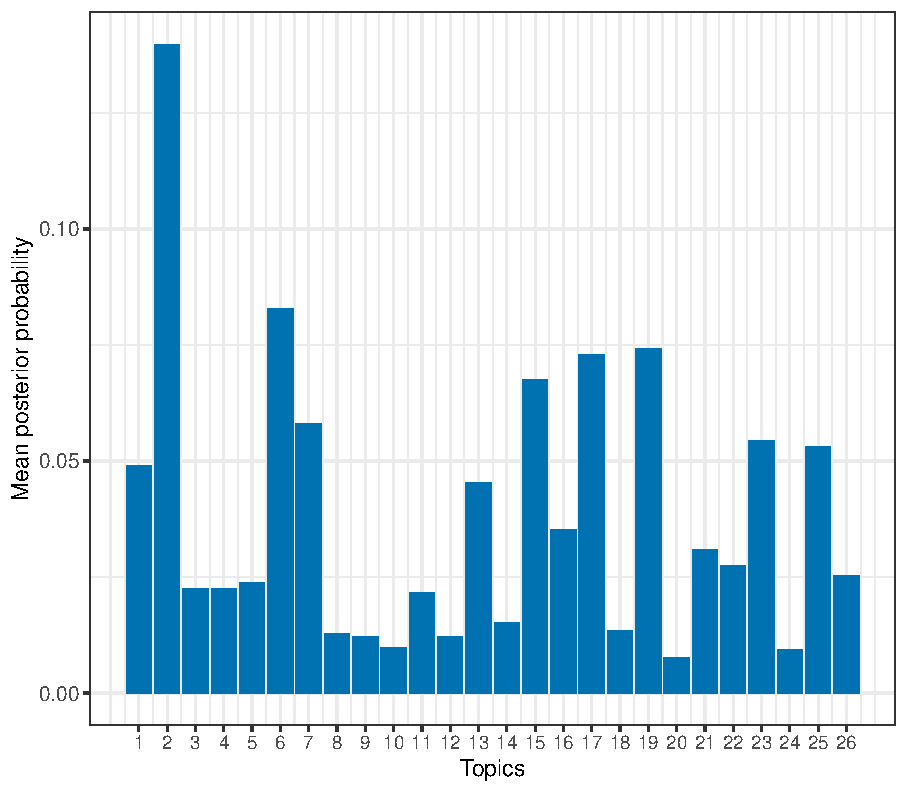
\includegraphics[width=\textwidth]{topic_prob_1991-2002.pdf}
        \caption{Mean posterior probabilities for the period 1991-2002.}
        \label{fig:topics_posterior1991}
    \end{subfigure}
    \hfill 
    \begin{subfigure}[b]{0.49\textwidth}
        \centering
        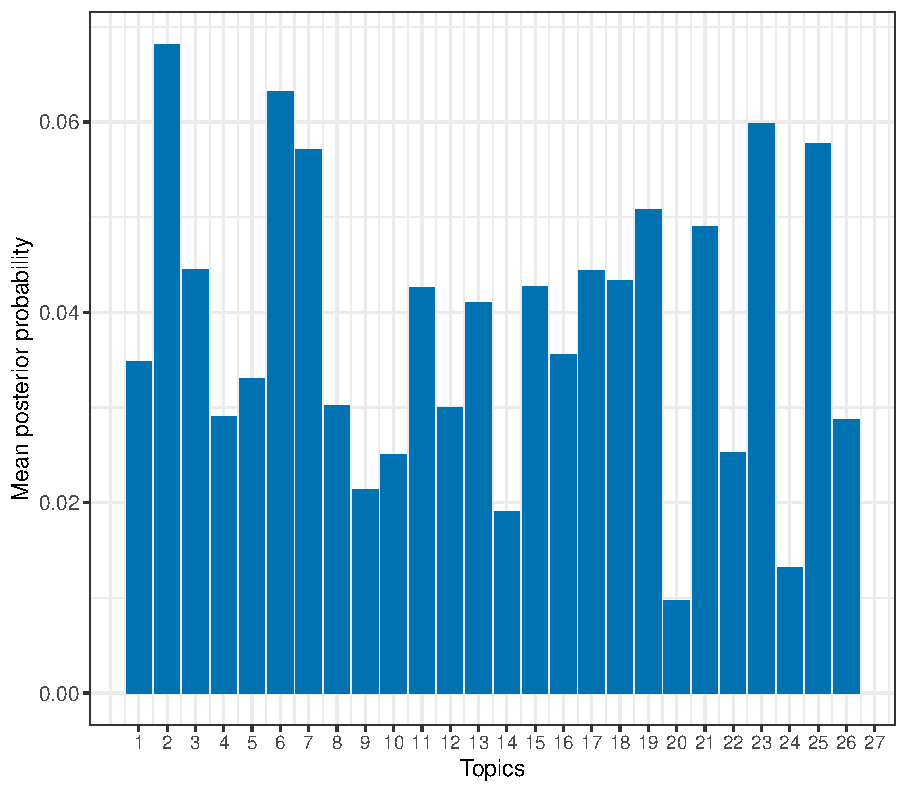
\includegraphics[width=\textwidth]{topic_prob_2003-2013.pdf}
        \caption{Mean posterior probabilities for the period 2003-2013.}
        \label{fig:topics_posterior2003}
    \end{subfigure}
    \hfill
    \begin{subfigure}[b]{0.49\textwidth}
        \centering
        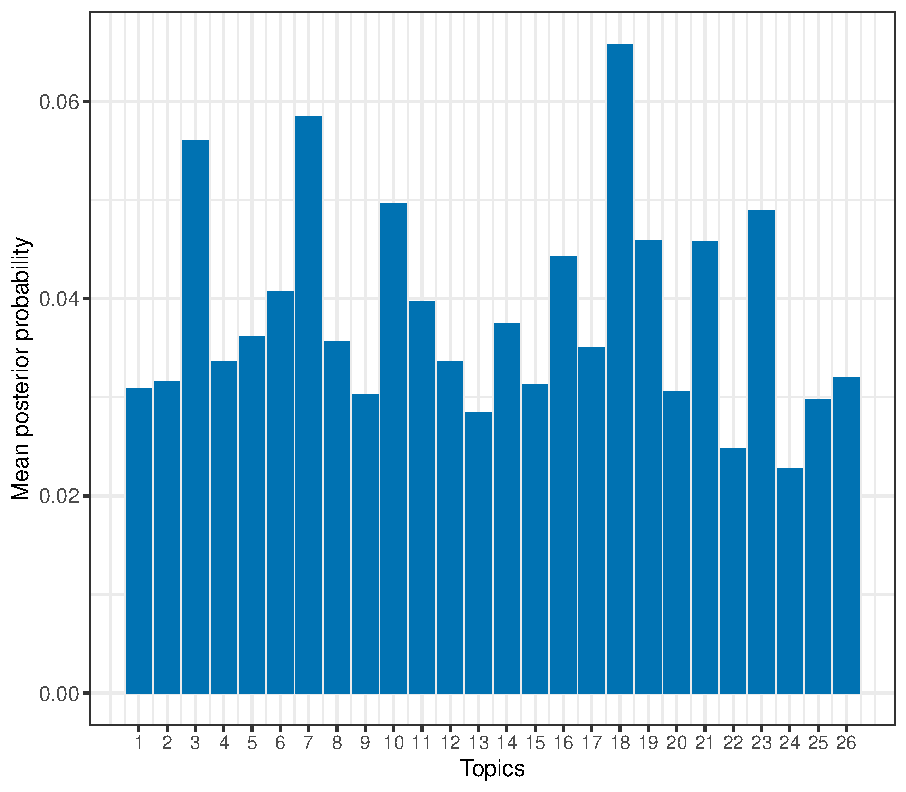
\includegraphics[width=\textwidth]{topic_prob_2014-2024.pdf}
        \caption{Mean posterior probabilities for the period 2014-2024.}
        \label{fig:topics_posterior2014}
    \end{subfigure}  
\caption{Mean posterior probability of the 26 topics for three periods.}
\label{fig:topics_posterior}
\end{figure}

The convergence of topic proportions we see in Figure \ref{fig:topics_posterior} can be better visualized plotting the mean posterior probabilities in a continuous time, like in Figures \ref{fig:topic_trends_1} and \ref{fig:topic_trends_2}. This convergence means in the mean posterior probability means that, if a scientific paper in the field of \textit{economics of migration} were to be produced today, it would be equally likely to be written on any of our 26 topics, which is a result that is only possible because the corpus we use to fit our LDA topic model is currently fairly diverse. However, our trend topic analysis shows that this was not always the case, especially in the period 1991-2002. Therefore, we see this convergence as an increase in the diversity in the field's topical structure, which confirms our hypothesis.

\begin{figure}[ht!]
	\centering
	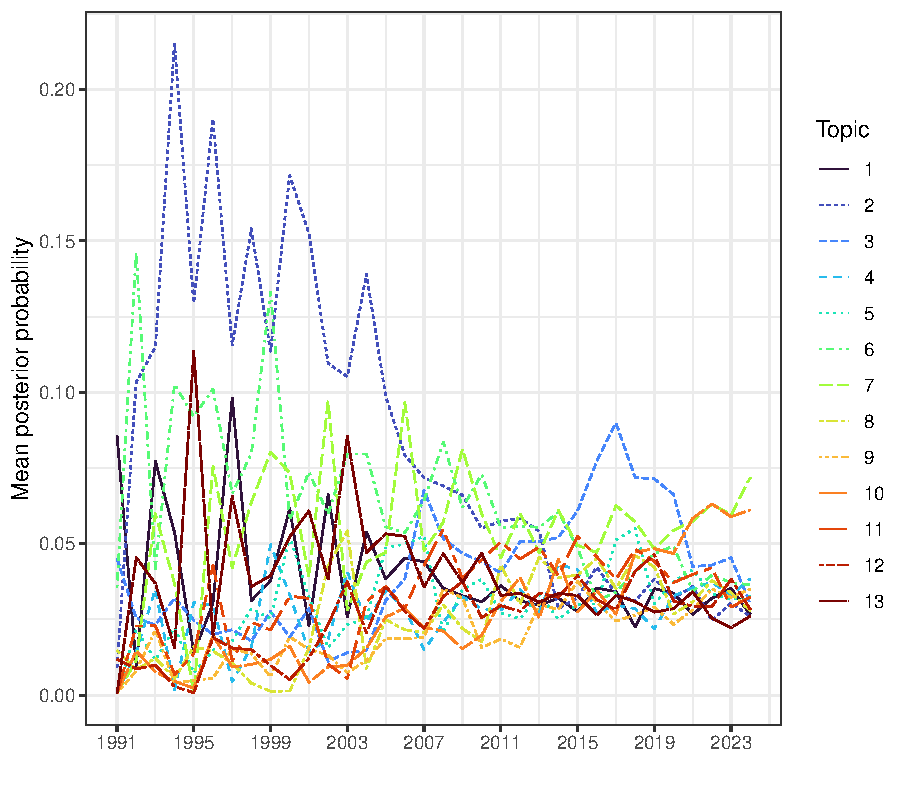
\includegraphics[scale=0.75]{topic_trends_1.pdf}
	\caption{Trends of topics 1 to 13 over the period 1991-2024.}
	\label{fig:topic_trends_1}
\end{figure}

\begin{figure}[ht!]
	\centering
	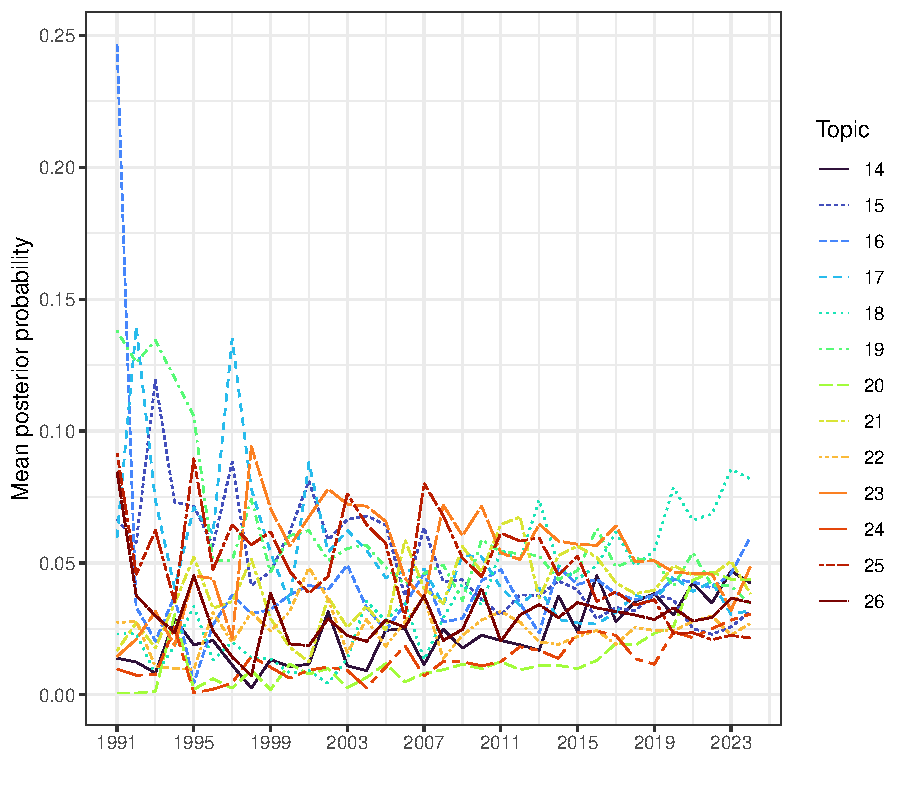
\includegraphics[scale=0.75]{topic_trends_2.pdf}
	\caption{Trends of topics 14 to 26 over the period 1991-2024.}
	\label{fig:topic_trends_2}
\end{figure}

\subsection{Diversity indices} \label{results_diversity_indices}

In order to validate the results of our trend topic analysis, we present two diversity indices, the Gini-Simpson and the Shannon-Wiener entropy indices, where the higher the values of both indices, the greater the diversity. As can be seen in Figures \ref{fig:gini_simpson_entropy} and \ref{fig:shannon_wiener_entropy}, both of our indices show that diversity in our corpus increased considerably between 1991 and 2009, reaching high levels of diversity, which have remained relatively stable since then. This result contrasts with that found by \cite[p. 467]{pisarevskaya_mapping_2020} in their analysis of diversity in the field of migration studies.

\begin{figure}[ht!]
	\centering
	\begin{subfigure}{0.49\textwidth}
		\centering
		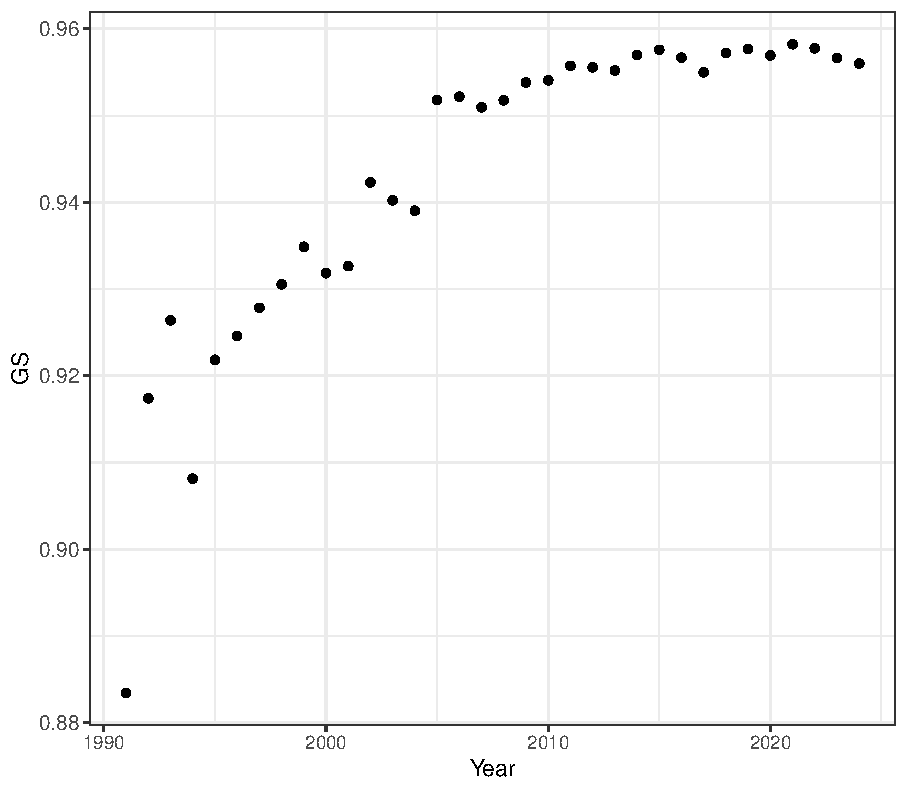
\includegraphics[scale=0.5]{gs_entropy.pdf}
		\caption{Gini-Simpson entropy index.}
		\label{fig:gini_simpson_entropy}
	\end{subfigure}
	\hfill
	\begin{subfigure}{0.49\textwidth}
		\centering
		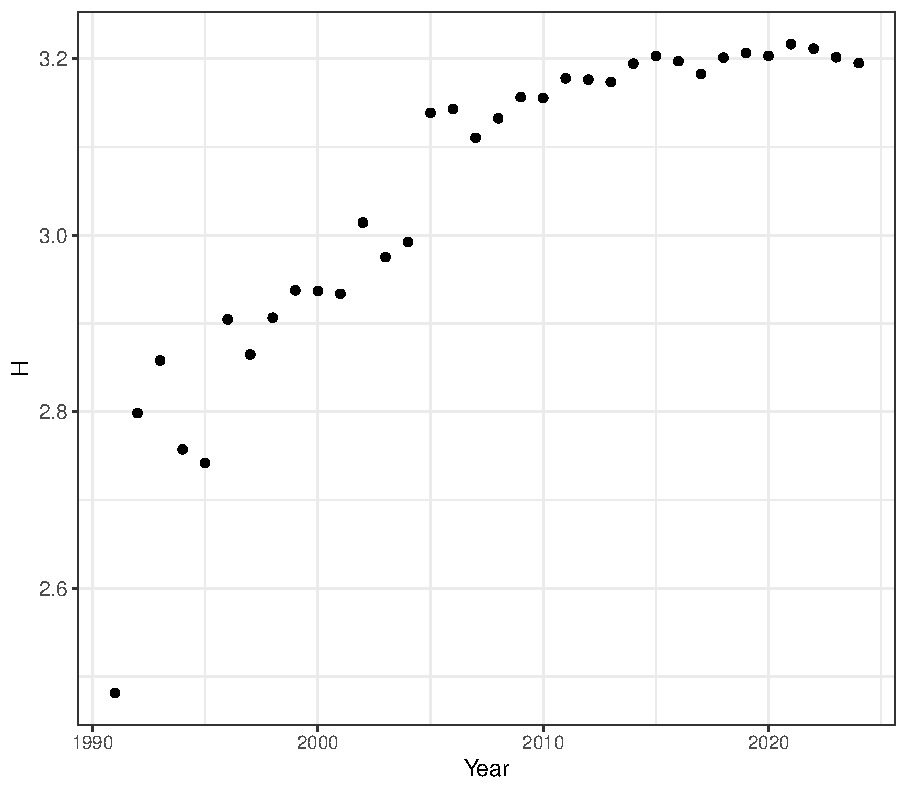
\includegraphics[scale=0.5]{h_entropy.pdf}
		\caption{Shannon-Wiener entropy index.}
		\label{fig:shannon_wiener_entropy}
	\end{subfigure}
\caption{Diversity measures.}
\label{fig:diversity_indices}
\end{figure}